% Author Name: José Areia 
% Author Contact: jose.apareia@gmail.com
% Version: 2.2.11 - 2025-08-28
% Public Repository: https://github.com/joseareia/ipleiria-thesis
% Wiki/Getting Help: https://github.com/joseareia/ipleiria-thesis/wiki

%%% Document Options %%%
\documentclass[
    language=spanish,
    docstage=final,
    media=paper,
    bookprint=false,
    linkcolor=blue!45!black,
    chapterstyle=classic,
    coverstyle=classic,
    aiacknowledgement=false,
    listprefix=false
]{ThesisUNAH}

%%% Colocación de figuras flotantes: se relajan las fracciones por defecto para que
%%% LaTeX empaque las figuras junto al texto y evite páginas casi vacías (menos huecos).
\renewcommand{\topfraction}{0.92}
\renewcommand{\bottomfraction}{0.88}
\renewcommand{\textfraction}{0.06}
\renewcommand{\floatpagefraction}{0.75}
\setcounter{topnumber}{2}
\setcounter{bottomnumber}{2}
\setcounter{totalnumber}{4}

%%% Document Version %%%
\DocumentVersion{1.0.0} 

%%% Document Metadata %%%
%% Custom Metadata for UNAH-style Cover Page
% This file contains all the information displayed on the custom cover

% ============================================
% CUSTOM COMMANDS FOR UNAH COVER
% ============================================

% --- Author Information ---
\newcommand{\GetCustomAuthor}{José Manuel Romero Martínez}

% --- Thesis Title ---
\newcommand{\GetCustomTitle}{%
    Aplicación móvil de traducción bidireccional \\[6pt]
    del Lenguaje de Señas Hondureño \\[6pt]
    mediante inteligencia artificial
}

% --- Thesis Type ---
\newcommand{\GetThesisTypeCustom}{Tesis de Pregrado}

% --- Faculty ---
\newcommand{\GetFaculty}{FACULTAD \\ \bfseries DE INGENIERÍA}

% --- Department ---
\newcommand{\GetDepartmentCustom}{DEPARTAMENTO DE INGENIERÍA\\ \bfseries EN SISTEMAS COMPUTACIONALES}

% --- Date ---
\newcommand{\GetCustomDate}{Julio del 2026}

% --- University Name (if needed elsewhere) ---
\newcommand{\GetCustomUniversity}{Universidad Nacional Autónoma de Honduras}

% --- Inspirational Quote ---
\newcommand{\GetQuote}{Confía en el Señor con todo tu corazón, y no te apoyes en tu propio entendimiento.}
\newcommand{\GetQuoteAuthor}{Proverbios 3:5}

% ============================================
% STANDARD COMMANDS (Required by system)
% ============================================

% First Author (Mandatory)
\FirstAuthor{José Manuel Romero Martínez}
%\FirstAuthorNumber{20181900636}

% Supervisor (Mandatory)
\AsesorMetodologico{PhD. Óscar Guillermo Hernández Ramírez}
\AsesorMetodologicoMail{oghernandez@unah.edu.hn}
\AsesorMetodologicoTitle{PhD., Universidad Nacional Autónoma de Honduras} 

%Co-Supervisor (Optional)
%\AsesorTecnico{MSc. Elías Emilio Flores Domínguez}
%\AsesorTecnicoMail{elias.florez@unah.edu.hn}
%\AsesorTecnicoTitle{MSc., Universidad Nacional Autónoma de Honduras}

% Autoridades Universitarias
\Rector{PhD. Odir Aarón Fernández Flores}
\SecretarioGeneral{Máster. José Alexander Ávila Vallecillo}
\VicerrectorAcademico{Dra. Lourdes Rosario Murcia Carbajal}
\DirectorCentro{Máster Milthon Moisés Reyes Sosa}
\SecretarioAcademico{Máster José Gámez Suazo}
\JefeDepartamento{PhD. Edis Francisco Romero Mejia}

% Title (Mandatory)
\Title{Aplicación móvil de traducción bidireccional del Lenguaje de Señas Hondureño mediante inteligencia artificial}

% University (Mandatory)
\University{Universidad Nacional Autónoma de Honduras}

% School (Mandatory)
\School{Facultad de Ingeniería}

% Department (Mandatory)
\Department{Departamento de Ingeniería en Sistemas Computacionales}

% Degree (Mandatory)
\Degree{Licenciatura en Ingeniería en Sistemas}

% Thesis Theme (Mandatory)
\ThesisType{Tesis de Pregrado}

% Local & Date (Mandatory)
\Date{Comayagua, Julio 2026}

% Academic Year 
\AcademicYear{2025}

% Custom Metadata for UNAH-style Cover Page
% This file contains all the information displayed on the custom cover

% ============================================
% CUSTOM COMMANDS FOR UNAH COVER
% ============================================

% --- Author Information ---
\newcommand{\GetCustomAuthor}{José Manuel Romero Martínez}

% --- Thesis Title ---
\newcommand{\GetCustomTitle}{%
    Aplicación móvil de traducción bidireccional \\[6pt]
    del Lenguaje de Señas Hondureño \\[6pt]
    mediante inteligencia artificial
}

% --- Thesis Type ---
\newcommand{\GetThesisTypeCustom}{Tesis de Pregrado}

% --- Faculty ---
\newcommand{\GetFaculty}{FACULTAD \\ \bfseries DE INGENIERÍA}

% --- Department ---
\newcommand{\GetDepartmentCustom}{DEPARTAMENTO DE INGENIERÍA\\ \bfseries EN SISTEMAS COMPUTACIONALES}

% --- Date ---
\newcommand{\GetCustomDate}{Julio del 2026}

% --- University Name (if needed elsewhere) ---
\newcommand{\GetCustomUniversity}{Universidad Nacional Autónoma de Honduras}

% --- Inspirational Quote ---
\newcommand{\GetQuote}{Confía en el Señor con todo tu corazón, y no te apoyes en tu propio entendimiento.}
\newcommand{\GetQuoteAuthor}{Proverbios 3:5}

% ============================================
% STANDARD COMMANDS (Required by system)
% ============================================

% First Author (Mandatory)
\FirstAuthor{José Manuel Romero Martínez}
%\FirstAuthorNumber{20181900636}

% Supervisor (Mandatory)
\AsesorMetodologico{PhD. Óscar Guillermo Hernández Ramírez}
\AsesorMetodologicoMail{oghernandez@unah.edu.hn}
\AsesorMetodologicoTitle{PhD., Universidad Nacional Autónoma de Honduras} 

%Co-Supervisor (Optional)
%\AsesorTecnico{MSc. Elías Emilio Flores Domínguez}
%\AsesorTecnicoMail{elias.florez@unah.edu.hn}
%\AsesorTecnicoTitle{MSc., Universidad Nacional Autónoma de Honduras}

% Autoridades Universitarias
\Rector{PhD. Odir Aarón Fernández Flores}
\SecretarioGeneral{Máster. José Alexander Ávila Vallecillo}
\VicerrectorAcademico{Dra. Lourdes Rosario Murcia Carbajal}
\DirectorCentro{Máster Milthon Moisés Reyes Sosa}
\SecretarioAcademico{Máster José Gámez Suazo}
\JefeDepartamento{PhD. Edis Francisco Romero Mejia}

% Title (Mandatory)
\Title{Aplicación móvil de traducción bidireccional del Lenguaje de Señas Hondureño mediante inteligencia artificial}

% University (Mandatory)
\University{Universidad Nacional Autónoma de Honduras}

% School (Mandatory)
\School{Facultad de Ingeniería}

% Department (Mandatory)
\Department{Departamento de Ingeniería en Sistemas Computacionales}

% Degree (Mandatory)
\Degree{Licenciatura en Ingeniería en Sistemas}

% Thesis Theme (Mandatory)
\ThesisType{Tesis de Pregrado}

% Local & Date (Mandatory)
\Date{Comayagua, Julio 2026}

% Academic Year 
\AcademicYear{2025}


%%% Loading of Glossary and Acronyms %%%
\makeglossaries
\loadglsentries{Matter/06-Glossary}
\loadglsentries[\acronymtype]{Matter/07-Acronyms}
\loadglsentries[\symboltype]{Matter/08-Symbols}

\begin{document}

%%% Front Matter %%%
% Custom Cover Page using TikZ
% Based on UNAH thesis template

% Define custom colors for this cover
\definecolor{amarilloTesis}{HTML}{FFD700}
\definecolor{azulFondo}{HTML}{2B3A64}

% Define Helvetica Neue font (or TeX Gyre Heros as fallback)
\newfontfamily\helveticaneue{TeX Gyre Heros}[
    UprightFont = *,
    BoldFont = * Bold,
    ItalicFont = * Italic,
    BoldItalicFont = * Bold Italic
]

% If Helvetica Neue is not available, use TeX Gyre Heros (Helvetica clone)
% Uncomment the line below if you don't have Helvetica Neue installed:
% \newfontfamily\helveticaneue{TeX Gyre Heros}

% Save current geometry
\newgeometry{left=0cm, right=0cm, top=0cm, bottom=0cm}

\begin{titlepage}
    \thispagestyle{empty}
    
    \begin{tikzpicture}[remember picture, overlay]
        
        % --- Background Image ---
        \node at (current page.center) {
            
\includegraphics[width=\paperwidth, height=\paperheight]{Figures/Theme/Cover.pdf}
        };
        
        % --- Thesis Title ---
        \node[
            text=black,
            font=\helveticaneue\bfseries\huge,
            align=left,
            text width=0.8\paperwidth,
            anchor=north west
        ] at ([xshift=2.5cm, yshift=-2.5cm]current page.north west)
        {\GetCustomTitle};
        
        % --- "Tesis de Pregrado" Label ---
        \node[
            text=amarilloTesis,
            font=\helveticaneue\bfseries\Huge,
            anchor=west
        ] at ([xshift=2.5cm, yshift=-10.5cm]current page.north west) {\GetThesisTypeCustom};
        
        % --- Faculty Block ---
        \node[
            text=white,
            font=\helveticaneue\footnotesize,
            align=left, 
            anchor=west
        ] at ([xshift=15.3cm, yshift=-9.5cm]current page.north west) {\GetFaculty};
        
        % --- Department Block ---
        \node[
            text=white,
            font=\helveticaneue\footnotesize,
            align=left,
            anchor=west
        ] at ([xshift=15.3cm, yshift=-10.8cm]current page.north west) {\GetDepartmentCustom};
        
        % --- Author Name ---
        \node[
            text=white,
            font=\helveticaneue\large,
            align=left,
            anchor=north west
        ] at ([xshift=2.5cm, yshift=-14cm]current page.north west) {
            Presentada por: \\
            \textcolor{amarilloTesis}{\bfseries\Large \GetCustomAuthor}
        };
        
        % --- Advisors Block ---
        \node[
            font=\helveticaneue\small,
            align=left,
            anchor=north west
        ] at ([xshift=12.5cm, yshift=-14cm]current page.north west) {
            \textcolor{amarilloTesis}{Asesor Metodológico:} \\
            \textcolor{white}{\GetAsesorMetodologico}
        };
        
        % --- Date (centered at bottom) ---
        \node[
            text=white,
            font=\helveticaneue\normalsize,
        ] at ([xshift=5cm, yshift=5.5cm]current page.south) {\GetCustomDate};
        
        % --- Decorative Illustration (bottom left) ---
        \node[
            anchor=south west, 
            xshift=1cm,      
            yshift=1cm       
        ] at (current page.south west) {
            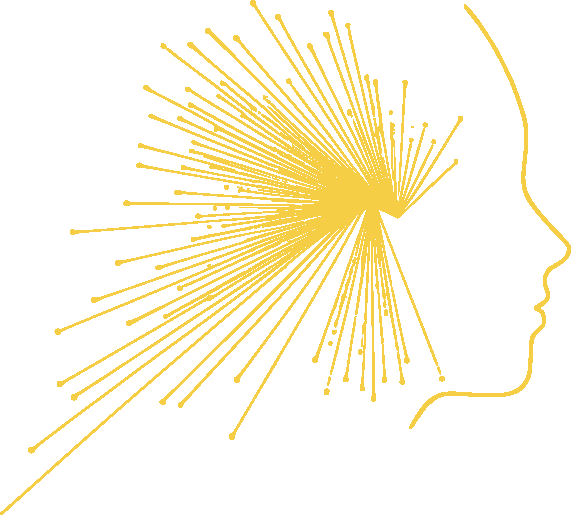
\includegraphics[width=10cm]{Figures/Theme/Ilustration.pdf} 
        };
        
        % --- University Logo (bottom right) ---
        \node[
            anchor=south east, 
            xshift=-0.5cm,      
            yshift=-0.5cm       
        ] at (current page.south east) {
            
\includegraphics[width=8cm]{Figures/Theme/Logotypes/backpage.pdf} 
        };
        
    \end{tikzpicture}
    
\end{titlepage}

% Restore geometry
\restoregeometry

\newcommand\BackgroundPicFrontPage{%
    \put(0,0){%
    \parbox[b][\paperheight]{\paperwidth}{%
    \vfill
    \centering
    
\includegraphics[width=\paperwidth,height=\paperheight]{Figures/Theme/Front-Page-S.pdf}%
    \vfill
}}}
\AddToShipoutPictureBG*{\BackgroundPicFrontPage}

\newgeometry{margin=1.98cm, top=2.15cm, bottom=1.47cm}
\begin{titlepage}
    \latofont
    \color{frontpagedark}
    \vspace*{\baselineskip}

    % Logo.
    \begin{figure}
        
\includegraphics[width=0.485\linewidth]{Figures/Theme/Logotypes/UNAH-Logo-C-Black.pdf}
    \end{figure}

    \vspace{3.5\baselineskip}

    % Title.
	\noindent
    \makebox[\textwidth][l]{%
        \parbox{\dimexpr\textwidth-2.5cm\relax}{
            \setstretch{1.03}
            \raggedright\bfseries\fontsize{20}{26}\selectfont\GetCustomTitle
        }
    }

    \vspace{0.8\baselineskip}


    \vspace{35pt}

    % Author.
    {\noindent\bfseries\fontsize{14}{19}\selectfont\GetFirstAuthor\orcid{0009-0001-0780-7160}}
    
    %{\noindent\itshape\fontsize{10}{10}\selectfont Número de Cuenta: \GetFirstAuthorNumber}

    \ifdefined\GetSecondAuthor
        \vspace{8pt}
        {\noindent\bfseries\fontsize{14}{19}\selectfont\GetSecondAuthor}
	\fi

    \ifdefined\GetThirdAuthor
        \vspace{8pt}
        {\noindent\bfseries\fontsize{14}{19}\selectfont\GetThirdAuthor}
	\fi

    \vfill    

    {
    \noindent
    \latofont
    \fontsize{10}{12}\selectfont
    \renewcommand{\arraystretch}{0.1}
    \hspace*{-2.5pt}\begin{tabular}{@{}r@{\hspace{5pt}}>{\raggedright\arraybackslash}m{6cm}@{}}
        \textbf{Asesor Metodológico:} & \GetAsesorMetodologico\orcid{0000-0003-3577-0411} \\ [-.7ex]
        & \setstretch{0.9}{\fontsize{8}{10}\selectfont\itshape \GetAsesorMetodologicoTitle} \\ [2ex]
        
        \ifdefined\GetAsesorTecnico
            \textbf{Asesor Técnico:} & \GetAsesorTecnico\orcid{0009-0006-8464-068X} \\ [-.7ex]
            & \setstretch{0.9}{\fontsize{8}{10}\selectfont\itshape \GetAsesorTecnicoTitle} \\ [.5ex]
        \fi

        \ifdefined\GetAsesorTecnicoSec        
            \textbf{Asesor Técnico Secundario:} & \GetAsesorTecnicoSec \\ [-.7ex]
            & \setstretch{0.9}{\fontsize{8}{10}\selectfont\itshape \GetAsesorTecnicoSecTitle} \\
        \fi
    \end{tabular}
    }
    
    \vfill
	
    % School.
	{\noindent\fontsize{10}{12}\selectfont\GetSchool}
	
    % Department.
	{\noindent\fontsize{10}{12}\selectfont\GetDepartment}

    % Degree.
	{\noindent\fontsize{10}{12}\selectfont\GetDegree}

    % Course.
    \ifdefined\GetCourse
        {\noindent\fontsize{10}{12}\selectfont\GetCourse}
	\fi

    \vspace{45pt}

    % Thesis option.
	{\noindent\fontsize{10}{12}\itshape\selectfont\GetThesisType}

    \vspace{45pt}

    % Local and date.
	{\noindent\fontsize{10}{12}\selectfont\GetDate}

    \vspace{68pt}
\end{titlepage}
\restoregeometry
\MediaOptionLogicBlank
\include{Matter/01a-Autoridades}
\chapter*{Acerca del Autor}

% ============================================
% PERFIL PRINCIPAL
% ============================================
\begin{tcolorbox}[colback=gray!5!white, colframe=blue!75!black]
	\begin{minipage}[c]{0.35\linewidth}
		\centering
		% Foto del autor — colocar imagen en Figures/carnet.png
		\setlength{\fboxsep}{0pt}
		\fbox{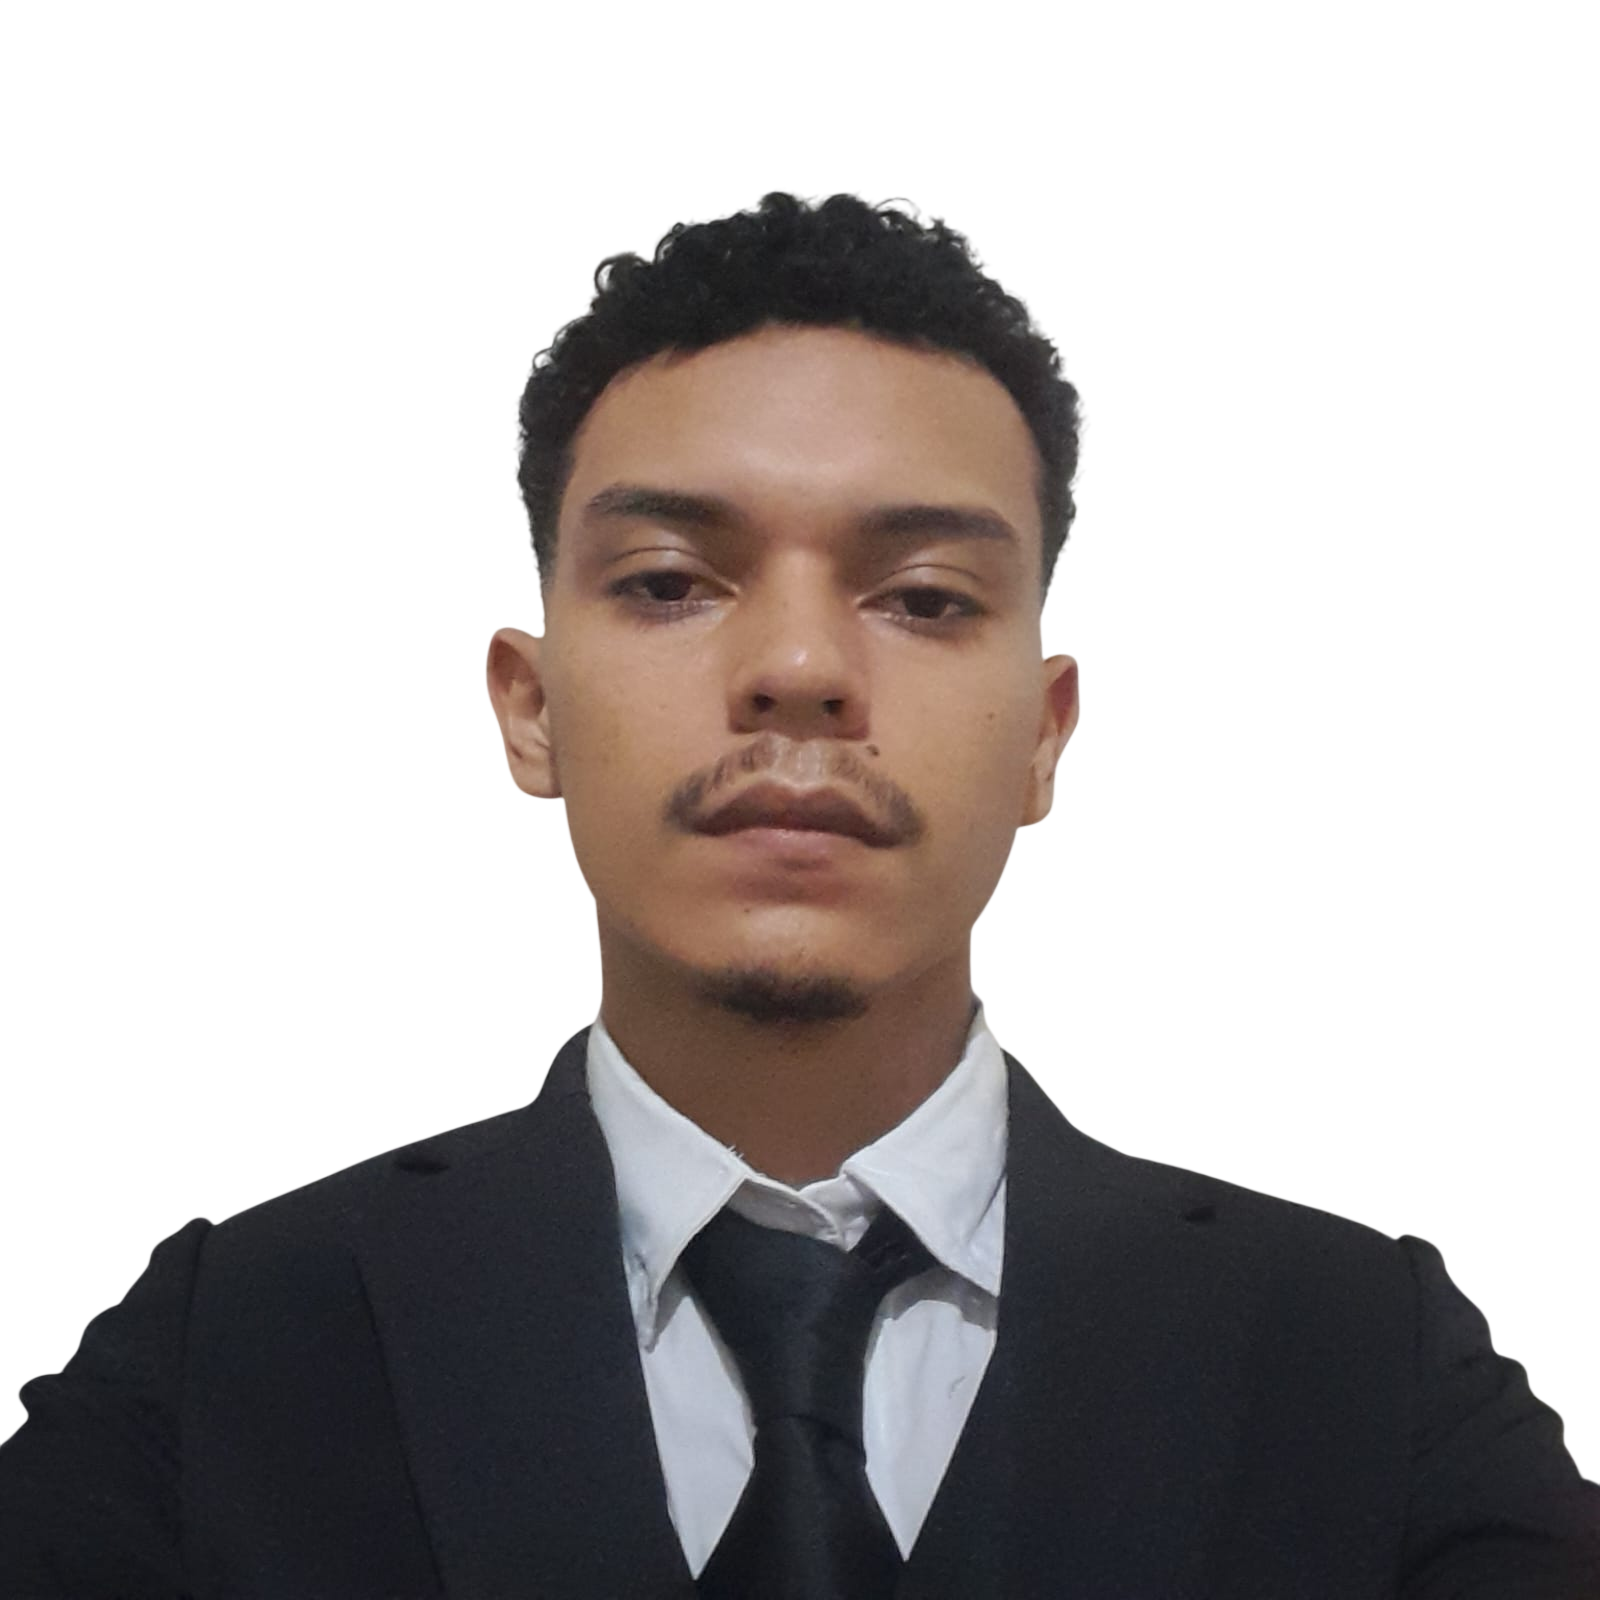
\includegraphics[width=\linewidth]{Figures/carnet.png}}
	\end{minipage}
	\hfill
	\begin{minipage}[c]{0.6\linewidth}
		\textbf{\large José Manuel Romero Martínez} \\[0.2cm]
		\textit{Estudiante de Ingeniería en Sistemas} \\
		Universidad Nacional Autónoma de Honduras \\
		Campus Comayagua

		\vspace{0.4cm}

		\begin{tabular}{@{}ll}
			\faOrcid\ ORCID: & \href{https://orcid.org/0009-0001-0780-7160}{0009-0001-0780-7160} \\[0.1cm]
			\faGraduationCap\ Google Scholar: & \href{https://scholar.google.com/citations?hl=es&user=uER9hnEAAAAJ}{José Manuel Romero Martínez} \\[0.1cm]
			\faLinkedin\ LinkedIn: & \href{https://www.linkedin.com/in/jos\%C3\%A9romero/}{/in/joséromero} \\[0.1cm]
			\faGithub\ GitHub: & \href{https://github.com/Josemaromero46}{@Josemaromero46} \\[0.1cm]
			\faEnvelope\ Email: & \href{mailto:romeromanuel@unah.hn}{romeromanuel@unah.hn}
		\end{tabular}
	\end{minipage}
\end{tcolorbox}

\vspace{0.4cm}

% ============================================
% RESEÑA BIOGRÁFICA
% ============================================
\noindent

Estudiante de Ingeniería en Sistemas en la Universidad Nacional Autónoma de Honduras, Campus
Comayagua. Su formación combina desarrollo de software, inteligencia artificial aplicada y
desarrollo móvil multiplataforma.

Ha participado en proyectos académicos y freelance en desarrollo móvil, \textit{backend} y
\textit{frontend}, trabajando con interfaces responsivas, componentes reutilizables y consumo
de \textit{APIs} REST. Entre sus proyectos destaca el desarrollo de una aplicación de torneos
de fútbol multiplataforma con Flutter y PocketBase. Cuenta además con experiencia en
configuración de redes y laboratorios universitarios.

\vspace{0.4cm}

% ============================================
% COMPETENCIAS TÉCNICAS
% ============================================
\noindent\textbf{Competencias Técnicas:}

\vspace{0.2cm}

\noindent
\textbf{Lenguajes:} C\#, C++, Java, Python, JavaScript, TypeScript, SQL, Prolog, \LaTeX{} \\
\textbf{Frontend:} HTML5, CSS3, Tailwind CSS, React, Next.js \\
\textbf{Frameworks:} Flutter, Node.js, Express.js, Firebase, Bootstrap, Spring \\
\textbf{Bases de datos:} MySQL, SQL Server, Oracle DB \\
\textbf{Herramientas:} Git, GitHub, Android Studio, VS Code, Figma, Canva \\
\textbf{Idiomas:} Español (nativo), Inglés (B1)

\MediaOptionLogic


%%% Copyright Statement %%%
\include{Matter/02-Copyright}

%%% Inspirational Quote %%%
\include{Matter/03-Quote}

%%% Dedication %%%
\pagenumbering{gobble} % Prevent page numbering.

\vspace*{\fill}

\begin{flushright}
    \textit{A Dios,\\
    por resguardarme en cada paso de este camino\\
    y darme la fortaleza para llegar hasta aquí.}

    \vspace{1em}

    \textit{A mis padres,\\
    por su amor incondicional y por todo el apoyo\\
    que nunca faltó. Este logro es tan suyo como mío.}
\end{flushright}

\vspace*{\fill}
\MediaOptionLogic


%%% Roman Numeration %%%
\pagenumbering{roman}

%%% Motivation %%%
\ifthenelse{\equal{\LanguageOption}{spanish}}{%
    \chapter*{Motivación}

    Las personas sordas en Honduras crecen aprendiendo el Lenguaje de Señas Hondureño como
    su primera lengua. Sin embargo, la escritura y la lectura del español se adquieren con el
    tiempo, a menudo ya en la adultez, y con un nivel de dominio que varía considerablemente
    de una persona a otra. Esto significa que, durante gran parte de su vida, muchas personas
    sordas solo pueden comunicarse con quienes conocen LESHO, y ese grupo es muy reducido
    dentro de la sociedad hondureña.

    El resultado es un aislamiento real y cotidiano. En una consulta médica, en una institución
    educativa, en una tienda, en cualquier espacio de la vida diaria, la persona sorda se
    enfrenta a una barrera que no depende de su capacidad ni de su voluntad, sino de la
    ausencia de un puente entre su lengua y la del entorno que la rodea.

    Esta situación fue la que motivó el presente trabajo. No parte de un interés técnico
    abstracto, sino de la convicción de que la tecnología puede y debe contribuir a reducir
    esa brecha. Construir una herramienta que permita a una persona sorda comunicarse con
    alguien que no conoce LESHO, sin depender de un intérprete y sin necesidad de conexión
    a internet, es un paso concreto hacia la inclusión. Pequeño en el contexto de todo lo que
    queda por hacer, pero real y necesario.
}{%
    \chapter*{Motivation}
    \guideinfo{In the \textit{Motivation} section, express your gratitude to those who helped and supported your work. Start by thanking your advisors, mentors, or supervisors who provided guidance and expertise. Mention any colleagues, classmates, or team members who contributed to discussions or offered assistance. You can also acknowledge specific organisations, institutions, or funding sources that supported your research or work. Lastly, include any personal acknowledgments for family or friends who offered encouragement and moral support during the project. Keep this section sincere, concise, and professional.}
}

\MediaOptionLogicBlank

%%% Acknowledgements %%%
\ifthenelse{\equal{\LanguageOption}{spanish}}{%
    \chapter*{Agradecimientos}

    A Dios, por ser la fuente de todo lo que soy. Ningún logro en mi vida tendría sentido
    sin reconocer que es Él quien me dio la inteligencia, la fortaleza y la capacidad de
    llegar hasta aquí. Sin su guía y su respaldo, nada de esto hubiese sido posible.

    A mi padre, \textbf{Víctor Manuel Romero Suazo}, por ser mi mayor ejemplo de esfuerzo
    y dedicación. Por enseñarme con su trabajo diario lo que significa no rendirse. Por ser
    ese hombre al que puedo acudir cuando el camino se complica, con la certeza de que
    encontrará la manera de ayudarme. Mi héroe de siempre.

    A mi madre, \textbf{Yelmy Jackeline Martínez Corea}, por ser mi mayor ejemplo de amor.
    Por estar siempre presente, por demostrarme con cada acción lo mucho que me quiere y
    lo mucho que cree en mí. Por su paciencia, por su esfuerzo y por ser ese apoyo que me
    ha sostenido en cada momento difícil. Todo lo que soy como persona lo debo, en gran
    parte, a ella.

}{%
    \chapter*{Acknowledgements}
    \guideinfo{In the \textit{Acknowledgements} section, express your gratitude to those who helped and supported your work. Start by thanking your advisors, mentors, or supervisors who provided guidance and expertise. Mention any colleagues, classmates, or team members who contributed to discussions or offered assistance. You can also acknowledge specific organisations, institutions, or funding sources that supported your research or work. Lastly, include any personal acknowledgments for family or friends who offered encouragement and moral support during the project. Keep this section sincere, concise, and professional.}
}

\MediaOptionLogicBlank

%%% Abstract %%%
\thispagestyle{plain}
\chapter*{Resumen}

La comunicación entre niños sordos y personas oyentes en Honduras presenta una brecha significativa, dado que el Lenguaje de Señas Hondureño (LESHO) es la lengua materna de la comunidad sorda y la mayoría de la población oyente no la conoce. Esta situación limita la capacidad de expresión y comprensión de los niños sordos en entornos cotidianos, sin que existan herramientas tecnológicas locales que aborden esta problemática de forma bidireccional.

La presente tesis propone el desarrollo de una aplicación móvil multiplataforma con dos módulos complementarios para la comunicación en tiempo real entre niños sordos y personas oyentes. El primero captura los gestos del niño a través de la cámara del dispositivo, extrae landmarks de las manos con MediaPipe Hands y los clasifica mediante dos modelos de aprendizaje profundo ejecutados en el dispositivo: una red neuronal convolucional en una dimensión para el reconocimiento del alfabeto dactilológico, y una red LSTM para el reconocimiento de señas dinámicas. El segundo módulo permite al oyente escribir en español y obtener la representación visual de la seña correspondiente mediante un muñeco animado que la reproduce, con un mecanismo de respaldo basado en el alfabeto dactilológico para palabras sin seña registrada. Para el entrenamiento se construyó un conjunto de datos propio de LESHO con la participación de personas con conocimiento de la lengua, que abarca el alfabeto completo y un vocabulario de señas dinámicas, almacenando únicamente coordenadas de landmarks.

Los resultados evidencian la viabilidad técnica de implementar un sistema de reconocimiento de señas on-device en aplicaciones móviles de bajo costo, sin dependencia de conectividad a internet, y con un diseño de interfaz orientado a usuarios infantiles. Este trabajo representa además un esfuerzo de construcción de un conjunto de datos de señas LESHO orientado al entrenamiento de modelos de inteligencia artificial, para el cual no se encontraron antecedentes documentados durante la revisión bibliográfica realizada.

\keywordses{Lengua de Señas Hondureña, LESHO, reconocimiento de gestos, MediaPipe, aprendizaje profundo, red neuronal convolucional, LSTM, aplicación móvil, Flutter, comunicación inclusiva, personas sordas}

\MediaOptionLogicBlank

\pdfbookmark[1]{Abstract}{abstract}
\chapter*{Abstract}

Communication between deaf children and hearing individuals in Honduras faces a significant gap, as Honduran Sign Language (LESHO) is the native language of the deaf community while most hearing people have no knowledge of it. This situation restricts the expressive and receptive capacities of deaf children in everyday contexts, with no local technological tools addressing this challenge in a bidirectional manner.

This thesis proposes a cross-platform mobile application with two complementary modules for real-time communication between deaf children and hearing individuals. The first captures the child's hand gestures via the device camera, extracts hand landmarks using MediaPipe Hands, and classifies them with two on-device deep learning models: a one-dimensional convolutional network for the dactylological alphabet, and an LSTM network for dynamic sign recognition. The second module allows hearing users to type in Spanish and receive a visual representation of the corresponding sign through an animated avatar that reproduces it, with a dactylological spelling fallback for words without a registered sign. A LESHO sign language dataset was built with the participation of individuals knowledgeable in the language, covering the full alphabet and a vocabulary of dynamic signs, storing only landmark coordinates.

Results demonstrate the technical feasibility of implementing an on-device sign language recognition system in low-cost mobile applications, without dependence on internet connectivity, and with an interface designed for child users. This work also represents an effort to build a LESHO sign language dataset oriented toward artificial intelligence model training, for which no documented precedents were found during the literature review conducted.

\keywordsen{Honduran Sign Language, LESHO, gesture recognition, MediaPipe, deep learning, convolutional neural network, LSTM, mobile application, Flutter, inclusive communication, deaf individuals}

\MediaOptionLogicBlank

%%% AI Acknowledgement %%%
%\include{Matter/08-AI}

%%% Table of Contents, List of Figures and List of Tables %%%
\dominitoc % Initialize minitoc
\bookmarktocentry\tableofcontents
\listoffigures
\listoftables

%%% Print: Glossary and Acronyms %%%
%%% \glossarytoc\printnormalglossary
\acronymtoc\printacronymglossary
%%% \symboltoc\printsymbolglossary

%%% Arabic Numeration %%%
\pagenumbering{arabic}

%%% Part 1: Presentación %%%
\include{Matter/Part-01}
\chapter[Presentación]{Presentación}
\label{cp:presentacion}

\insertminitoc
\parindent0pt

\section{Planteamiento del Problema}

Según la Organización Mundial de la Salud (\acrshort{oms}), más de 1\,500 millones de personas en
el mundo presentan algún grado de pérdida auditiva, de las cuales aproximadamente 430
millones requieren atención especializada. De este total, se estima que al menos 34 millones
son niños \cite{who_deafness_2024}. Para esta población, la lengua de señas constituye el principal medio de
comunicación y expresión, configurando una forma de interacción con valores y costumbres
propias que difieren de las de la población oyente.

En Honduras, la comunidad sorda está organizada en torno a la Asociación de Sordos de
Honduras (\acrshort{ash}), institución que ha impulsado el desarrollo y la documentación del
Lenguaje de Señas Hondureño (\acrshort{lesho}), el cual fue reconocido oficialmente como la lengua
natural de la comunidad sorda mediante el Decreto Legislativo No. 321-2013 \cite{congreso_decreto_2013}, \cite{ash_diccionario_2019}. Sin
embargo, según datos de la Comisión Nacional de los Derechos Humanos (\acrshort{conadeh}),
en Honduras existen aproximadamente 100\,000 personas con discapacidad auditiva, de las
cuales únicamente alrededor del 1\,\% cuenta con un carné oficial de identificación, lo que
evidencia el bajo nivel de reconocimiento institucional de esta población \cite{conadeh_discriminados}.

La brecha de comunicación entre niños sordos y personas oyentes se manifiesta en
prácticamente todos los entornos cotidianos, incluyendo el hogar, la comunidad y los
espacios de atención en salud. La mayoría de los niños sordos nacen en hogares de padres
oyentes que no conocen el \acrshort{lesho}, lo que retrasa el acceso temprano a una lengua completa
y limita su desarrollo socioemocional \cite{williams_encuesta_2015}. A esto se suma la escasez de intérpretes
certificados fuera de entornos educativos especializados, especialmente en zonas rurales
o de bajos recursos donde su presencia es prácticamente inexistente.

A pesar de que existen soluciones tecnológicas para el reconocimiento de otras lenguas de
señas, como la Lengua de Señas Americana o la Lengua de Señas Brasileña, no existe a la
fecha una aplicación móvil que permita a un niño sordo expresarse en \acrshort{lesho} hacia una
persona oyente en tiempo real, ni que facilite la comunicación en la dirección inversa
representando el español de forma visual en la lengua materna del niño. Las herramientas
comerciales disponibles no contemplan el vocabulario ni las particularidades del \acrshort{lesho}, y
su idioma de interfaz y su costo representan barreras adicionales para la población
hondureña \cite{sadik_survey_2025}.

\subsection{Preguntas de Investigación}

¿Es posible desarrollar una aplicación móvil que reconozca gestos del Lenguaje de Señas
Hondureño en tiempo real utilizando visión por computadora y aprendizaje profundo
ejecutado directamente en el dispositivo?

¿Puede una solución bidireccional facilitar la comunicación entre niños sordos y personas
oyentes sin requerir conocimiento previo del \acrshort{lesho} por parte de ninguna de las dos partes?

¿Qué nivel de precisión y usabilidad puede alcanzar un sistema de este tipo desarrollado
con un conjunto de datos propio de \acrshort{lesho} de alcance acotado?

\subsection{Justificación del Estudio}

La igualdad en la comunicación es un derecho que debe garantizarse para todas las
personas. Los niños sordos en Honduras enfrentan barreras cotidianas que van más allá
del ámbito educativo, afectando su capacidad de expresarse y comprender en entornos
familiares, comunitarios y de salud. La dependencia exclusiva de intérpretes humanos
profundiza esta desigualdad en contextos donde su presencia es escasa o inexistente \cite{congreso_decreto_2013}.

La relevancia de este trabajo radica en explorar una solución tecnológica contextualizada
a la realidad hondureña, dado que la mayoría de herramientas existentes han sido diseñadas
para otras lenguas de señas y otros entornos. El desarrollo de una aplicación móvil
bidireccional que opere sin conexión a internet es especialmente pertinente en un país
con cobertura de datos móviles desigual, donde no puede garantizarse el acceso a servicios
en la nube de forma permanente.

El estudio tiene impacto tanto académico como social. Desde el punto de vista académico,
la construcción de un conjunto de datos de señas del \acrshort{lesho} orientado al entrenamiento de modelos
de inteligencia artificial constituye un aporte al campo tecnológico local, ya que durante
la revisión bibliográfica realizada no se encontraron antecedentes documentados de un
recurso de este tipo para esta lengua.
Desde el punto de vista social, la aplicación busca reducir la brecha de comunicación entre
niños sordos y personas oyentes, aportando una herramienta de inclusión comunicativa
de bajo costo y sin dependencia de infraestructura externa.

\subsection{Viabilidad del Estudio}

La viabilidad del estudio se analiza en función de los siguientes puntos.

\begin{enumerate}
    \item Disponibilidad de recursos.
    \begin{itemize}
        \item \textbf{Humanos:} la investigación será desarrollada por el tesista con la guía del asesor
        correspondiente, y contará con la colaboración de personas con conocimiento de
        \acrshort{lesho} vinculadas a fundaciones de atención a personas con discapacidad en el
        departamento de Comayagua.
        \item \textbf{Tecnológicos:} se dispone de herramientas de código abierto para el desarrollo,
        incluyendo Flutter, MediaPipe y TensorFlow Lite, las cuales no requieren licencias
        de pago y cuentan con documentación oficial extensa \cite{google_mediapipe_2024}, \cite{google_tflite_2024}, \cite{google_flutter_2024}.
        \item \textbf{Datos:} el conjunto de datos de señas será construido durante la investigación siguiendo un
        protocolo de captura documentado, con referencia al diccionario de \acrshort{lesho}
        publicado por la \acrshort{ash} \cite{ash_diccionario_2019}.
    \end{itemize}

    \item Alcance del estudio.

    La investigación se centrará en desarrollar una aplicación móvil funcional que
    reconozca el alfabeto dactilológico y un vocabulario de 50 señas dinámicas, y que
    permita representar visualmente señas del \acrshort{lesho} a partir de texto en español. El
    estudio no pretende abarcar la totalidad del vocabulario del \acrshort{lesho} ni contempla
    aspectos gramaticales como expresiones faciales o lenguaje corporal. La evaluación
    se realizará en condiciones controladas con usuarios con conocimiento de la lengua.

    \item Implicaciones del estudio.
    \begin{itemize}
        \item \textbf{Académicas:} contribuye al conocimiento en el campo del reconocimiento de gestos
        y la accesibilidad tecnológica aplicada a la comunidad sorda hondureña.
        \item \textbf{Tecnológicas:} promueve el desarrollo de soluciones con inteligencia artificial
        ejecutada en el dispositivo, sin dependencia de servidores externos.
        \item \textbf{Sociales:} fomenta la inclusión comunicativa de niños sordos en entornos
        cotidianos, aportando una herramienta accesible y de bajo costo.
    \end{itemize}

    \item Consecuencias del estudio.

    Los resultados obtenidos pueden servir como base para investigaciones futuras que
    amplíen el vocabulario reconocido, incorporen componentes no manuales del \acrshort{lesho}
    o extiendan la solución a otros contextos de uso. La metodología de construcción
    del conjunto de datos y el proceso de entrenamiento de modelos quedan documentados de
    forma reproducible para facilitar su extensión.
\end{enumerate}

\section{Objetivo General}

Desarrollar una aplicación de inteligencia artificial para la comunicación entre niños
sordos y oyentes mediante el reconocimiento de señas \acrshort{lesho}, ejecutada de forma
completamente local en el dispositivo móvil.

\section{Objetivos Específicos}

\begin{enumerate}
    \item Recopilar un conjunto de datos de señas \acrshort{lesho} que incluya el alfabeto dactilológico
    completo y un vocabulario de señas dinámicas de uso cotidiano, siguiendo un protocolo
    de captura documentado y reproducible.

    \item Diseñar e implementar modelos de clasificación de señas estáticas y dinámicas
    optimizados para su ejecución en dispositivos móviles con recursos computacionales
    limitados.

    \item Desarrollar una aplicación que integre el reconocimiento automático de señas y un
    diccionario visual de señas pregrabadas, operando sin dependencia de servicios en la
    nube.

    \item Evaluar el desempeño técnico del sistema en términos de exactitud de clasificación y
    latencia de inferencia, y valorar la usabilidad de la aplicación mediante pruebas con
    usuarios que incluyan personas con conocimiento de \acrshort{lesho}.
\end{enumerate}


%%% Part 2: Marco Teórico %%%
\include{Matter/Part-02}
\include{Chapters/Investigaciones-Previas}
\chapter{Discapacidad Auditiva y Comunidad Sorda}
\label{cp:discapacidad-auditiva}

\insertminitoc
\parindent0pt

Para comprender el contexto en que se desarrolla esta investigación, es necesario examinar
la discapacidad auditiva desde dos perspectivas complementarias: la médica, que permite
entender sus causas, clasificación y prevalencia, y la sociocultural, que reconoce a las
personas sordas como miembros de una comunidad lingüística con identidad propia. Este
capítulo aborda ambas perspectivas, con especial atención a la situación de los niños
sordos, las barreras de comunicación que enfrentan con la población oyente y el contexto
específico de Honduras donde se enmarca la investigación.

\section{Discapacidad Auditiva: Definición, Clasificación y Prevalencia}

La pérdida auditiva se define como la disminución parcial o total de la capacidad de
percibir sonidos. La Organización Mundial de la Salud (\acrshort{oms}) clasifica la pérdida auditiva
en grados según el umbral de audición medido en decibelios (dB), evaluado mediante el
promedio de tonos puros en las frecuencias de 500, 1000, 2000 y 4000 Hz. La
Tabla~\ref{tab:clasificacion-perdida-auditiva} resume la clasificación vigente, que
distingue siete grados que van desde la audición normal hasta la pérdida completa.

\begin{table}[h!]
\centering
\begin{tabular}{lc}
\hline
\textbf{Grado de pérdida auditiva} & \textbf{Umbral de audición (dB)} \\
\hline
Audición normal & -10.0 a 19.9 \\
Pérdida leve & 20.0 a 34.9 \\
Pérdida moderada & 35.0 a 49.9 \\
Pérdida moderadamente severa & 50.0 a 64.9 \\
Pérdida severa & 65.0 a 79.9 \\
Pérdida profunda & 80.0 a 94.9 \\
Pérdida completa & 95.0 o superior \\
\hline
\end{tabular}
\caption[Clasificación de la pérdida auditiva según la OMS]{Clasificación de la pérdida auditiva según la \acrshort{oms}, por grado y umbral de audición. Fuente: elaboración propia a partir de \cite{olusanya_hearing_2019}.}
\label{tab:clasificacion-perdida-auditiva}
\end{table}

Como se observa en la Tabla~\ref{tab:clasificacion-perdida-auditiva}, cada grado
corresponde a un rango del umbral auditivo, de manera que a mayor umbral en decibelios
mayor es la pérdida. Sobre la base de esta escala, la \acrshort{oms} considera como pérdida
auditiva discapacitante aquella superior a 40 dB en adultos y superior a 30 dB en niños \cite{who_deafness_2024}.

En términos de prevalencia, el Informe Mundial sobre la Audición publicado por la \acrshort{oms}
en 2021 estima que más de 1\,500 millones de personas en el mundo presentan algún grado
de pérdida auditiva, de las cuales aproximadamente 430 millones requieren atención
especializada \cite{who_world_report_2021}. De este total, se estima que 34 millones son niños \cite{who_deafness_2024}. El informe proyecta
que, sin intervenciones preventivas adecuadas, para el año 2050 cerca de 2\,500 millones de
personas vivirán con algún grado de pérdida auditiva y al menos 700 millones necesitarán
servicios de rehabilitación \cite{who_world_report_2021}.

La pérdida auditiva puede ser de origen congénito o adquirido. Entre las causas congénitas
se encuentran factores genéticos, complicaciones durante el embarazo y el parto, bajo peso
al nacer y la ictericia neonatal. Entre las causas adquiridas destacan las infecciones crónicas
del oído, la exposición prolongada a ruidos intensos, el uso de medicamentos ototóxicos y
el envejecimiento \cite{who_deafness_2024}. En el caso de los niños, aproximadamente 200 millones padecen
infecciones crónicas del oído que pueden prevenirse o tratarse, lo que subraya la
importancia de la intervención temprana \cite{who_world_report_2021}.

\section{La Comunidad Sorda y la Cultura Visual}

Las personas sordas conforman una comunidad con una identidad cultural y lingüística
propia que trasciende la condición audiológica. La Federación Mundial de Sordos (\acrshort{wfd}),
organización internacional que representa aproximadamente a 70 millones de personas
sordas en 135 países, ha sostenido de forma consistente que las personas sordas no se
definen por una condición médica deficitaria, sino por su pertenencia a una minoría
lingüística y cultural cuyo rasgo central es el uso de una lengua de señas nacional \cite{wfd_cultural_2018}.

La Convención sobre los Derechos de las Personas con Discapacidad (\acrshort{cdpd}) de las
Naciones Unidas reconoce en su Artículo 30 que las personas con discapacidad tienen
derecho al reconocimiento y apoyo de su identidad cultural y lingüística específica,
incluyendo las lenguas de señas y la cultura sorda \cite{onu_cdpd_2006}. La \acrshort{wfd} ha señalado que este
reconocimiento implica una interseccionalidad singular: las personas sordas pertenecen
simultáneamente al ámbito de la discapacidad y al de las minorías lingüísticas, una
condición que no comparten otros grupos \cite{wfd_sign_language_rights_2024}.

La comunicación en la comunidad sorda se organiza en torno a la modalidad visual y
gestual. A diferencia de las lenguas orales, que operan en el canal auditivo-vocal, las
lenguas de señas utilizan el canal visual-gestual, lo que implica una organización espacial
del lenguaje. Esta diferencia no representa una limitación, sino una modalidad alternativa
igualmente compleja y expresiva. Las lenguas de señas nacionales se originan en las
comunidades sordas y se desarrollan con ellas, por lo que cada país o región puede tener
su propia lengua de señas, con gramática y vocabulario independientes de la lengua oral
del mismo territorio \cite{wfd_primacy_2024}.

\section{La Infancia Sorda y el Acceso Temprano a la Lengua de Señas}

La adquisición del lenguaje en los primeros años de vida constituye un proceso
determinante para el desarrollo cognitivo, emocional y social de cualquier niño. Humphries
et al. documentaron que los niños adquieren el lenguaje sin instrucción formal siempre que
estén expuestos de manera regular y significativa a una lengua humana accesible. Sin
embargo, debido a los cambios en la plasticidad cerebral durante la primera infancia, los
niños que no adquieren una primera lengua en los primeros años podrían no alcanzar nunca
una competencia lingüística plena en ningún idioma \cite{humphries_language_2012}.

Este fenómeno, conocido como deprivación lingüística, tiene consecuencias directas sobre
el desarrollo de actividades cognitivas que dependen de una base lingüística sólida, como
la lectoescritura, la organización de la memoria y la manipulación numérica \cite{humphries_language_2012}. La
adquisición de una lengua de señas está sujeta a las mismas restricciones temporales que
la adquisición de una lengua oral: si el niño sordo no accede a una lengua de señas durante
el período crítico, las consecuencias sobre su desarrollo lingüístico pueden ser permanentes.

La \acrshort{wfd} ha enfatizado en su documento de posición sobre los derechos lingüísticos de los
niños sordos que la necesidad de adquisición natural del lenguaje a través de una lengua
de señas es un derecho fundamental de todos los niños sordos, y que los métodos
educativos que mejor promueven el desarrollo de su identidad cultural y lingüística son los
modelos bilingües con lengua de señas completa \cite{wfd_language_rights_2016}.

A pesar de la evidencia científica, Humphries et al. señalaron que el 80\,\% de los niños
sordos nacen en familias oyentes, lo que con frecuencia retrasa o impide el acceso temprano
a una lengua de señas \cite{humphries_language_2012}. Esta situación es especialmente grave en países en desarrollo
donde los servicios de detección temprana, los programas de intervención y la disponibilidad
de profesionales en lengua de señas son limitados o inexistentes.

\section{Barreras de Comunicación con Personas Oyentes}

La barrera fundamental entre la comunidad sorda y la oyente radica en la asimetría
lingüística: mientras que las personas sordas necesitan la lengua de señas como medio
principal de comunicación, la mayoría de la población oyente no la conoce. Esta asimetría
genera exclusión en múltiples ámbitos de la vida cotidiana.

En el entorno educativo, la escasez de intérpretes de lengua de señas y de docentes con
competencia en la lengua constituye una de las barreras más documentadas. La \acrshort{cdpd}
establece en su Artículo 24 la obligación de los Estados de asegurar que la educación de
las personas sordas se imparta en las lenguas y los modos y medios de comunicación más
apropiados, y en entornos que permitan alcanzar su máximo desarrollo académico y
social \cite{onu_cdpd_2006}.

En el entorno familiar, la barrera se origina desde el nacimiento cuando el niño sordo nace
en una familia oyente que no conoce la lengua de señas. La comunicación temprana se ve
restringida a gestos naturales y estrategias ad hoc que no constituyen un sistema
lingüístico completo, lo que afecta el vínculo afectivo y la transmisión cultural entre padres
e hijos \cite{humphries_language_2012}.

En el entorno comunitario y de servicios, las personas sordas enfrentan dificultades para
acceder a servicios básicos de salud, trámites legales y atención de emergencias. La
ausencia de mecanismos de comunicación accesibles obliga a depender de familiares como
intermediarios, lo que compromete la privacidad y la autonomía de la persona sorda. La
tecnología móvil ha sido señalada como una vía prometedora para reducir estas barreras,
siempre que las soluciones estén adaptadas a la lengua de señas local y sean accesibles
económicamente \cite{who_world_report_2021}.

\section{Situación de las Personas Sordas en Honduras}

Luego de revisar el panorama general de la discapacidad auditiva y sus implicaciones
comunicativas y educativas, es necesario situar esa realidad en el contexto hondureño,
que es donde se desarrolla y hacia donde se dirigen los resultados de esta investigación.

En Honduras, la Comisión Nacional de los Derechos Humanos (\acrshort{conadeh}) ha reportado
que existen aproximadamente 100\,000 personas con discapacidad auditiva en el país. Sin
embargo, únicamente alrededor del 1\,\% de esta población cuenta con un carné oficial de
identificación como persona con discapacidad, lo que evidencia un bajo nivel de
reconocimiento institucional y un acceso limitado a los servicios y beneficios a los que
tienen derecho \cite{conadeh_discriminados}.

Williams y Parks, en una encuesta sociolingüística realizada para SIL International,
documentaron que la comunidad sorda hondureña se comunica a través del Lenguaje de
Señas Hondureño (\acrshort{lesho}) y que más de 3\,000 personas han recibido formación en esta
lengua a través de cursos ofrecidos por la Asociación de Sordos de Honduras (\acrshort{ash}) y la
Universidad Nacional Autónoma de Honduras (\acrshort{unah}). El estudio también registró
variaciones regionales en el \acrshort{lesho} y señaló que la mayoría de las personas sordas
aprenden la lengua a través de su escuela o de las clases impartidas por la \acrshort{ash} \cite{williams_encuesta_2015}.

En el ámbito educativo, la \acrshort{unah} ha ofrecido cursos de \acrshort{lesho} de forma ininterrumpida
durante más de 23 años, y en 2024 el Programa de Servicios a Estudiantes con Necesidades
Especiales (\acrshort{prosene}) lanzó el Diccionario Digital de \acrshort{lesho} con más de 700 señas en
formato de video, orientado inicialmente al vocabulario del entorno universitario. El
diccionario fue desarrollado por personal y estudiantes sordos adscritos al \acrshort{prosene} y
constituye el primer recurso digital de su tipo para esta lengua \cite{unah_diccionario_2024}.

A pesar de estos avances, el acceso a intérpretes certificados fuera del ámbito educativo
universitario sigue siendo escaso, especialmente en zonas rurales y ciudades intermedias.
No existen a la fecha herramientas tecnológicas locales que permitan la comunicación
autónoma en tiempo real entre personas sordas y oyentes sin la intermediación de un
intérprete humano.

\chapter{Lengua de Señas Hondureña (LESHO)}
\label{cp:lesho}

\insertminitoc
\parindent0pt

El capítulo anterior estableció que las personas sordas conforman una comunidad
lingüística cuya lengua materna es la lengua de señas. En Honduras, esa lengua es el
Lenguaje de Señas Hondureño (\acrshort{lesho}), que constituye a la vez el objeto de reconocimiento
y el medio de comunicación que esta investigación busca apoyar. Este capítulo describe sus
características fundamentales: su historia y reconocimiento oficial, los parámetros que
componen las señas, la distinción entre señas estáticas y dinámicas, el alfabeto
dactilológico y su gramática en relación con el español.

\section{Origen, Evolución y Reconocimiento Oficial}

El Lenguaje de Señas Hondureño (\acrshort{lesho}) es la lengua natural de la comunidad sorda de
Honduras. Su proceso de documentación formal se inició en 1983 con la publicación del
primer diccionario impreso de lengua de señas en el país, denominado ``Las Manos Hablan'',
elaborado en el seno de la Asociación de Sordos de Honduras (\acrshort{ash}). A esta obra le
sucedieron una segunda edición en 2005, titulada ``Comuniquemos Mejor'', y una tercera
en 2019, denominada ``Diccionario de \acrshort{lesho} Tomo I, Primera Edición'', que documenta más
de 900 señas \cite{ash_diccionario_2019}.

El reconocimiento oficial del \acrshort{lesho} se concretó mediante el Decreto Legislativo
No. 321-2013, aprobado por el Congreso Nacional de Honduras, que estableció la Ley de la
Lengua de Señas Hondureña. Esta ley reconoce el \acrshort{lesho} como un derecho en beneficio de
las personas sordas, con discapacidad auditiva y sordociegas que libremente decidan
utilizarla como medio o sistema lingüístico para comunicarse, y obliga al Estado a promover
su uso en los ámbitos educativo, institucional y social \cite{congreso_decreto_2013}.

Williams y Parks documentaron en su encuesta sociolingüística que el \acrshort{lesho} presenta
variaciones regionales, especialmente entre ciudades como Tegucigalpa, San Pedro Sula y
La Ceiba. A pesar de estas variaciones, el estudio determinó que existe un alto grado de
similitud léxica entre las distintas regiones, con coincidencias superiores al 74\,\% en
comparaciones entre diccionarios. La estandarización de la lengua ha sido impulsada
principalmente por la \acrshort{ash} y por los cursos de \acrshort{lesho} ofrecidos en instituciones educativas
del país \cite{williams_encuesta_2015}.

\section{Parámetros Formacionales de las Señas}

Al igual que las lenguas orales se descomponen en unidades mínimas sin significado propio
llamadas fonemas, las lenguas de señas también poseen una estructura fonológica
compuesta por unidades formacionales. Esta noción fue establecida por William Stokoe en
1960, cuyo trabajo demostró que las señas no son gestos holísticos e indivisibles, sino que
se componen de un conjunto finito de elementos sin significado que se combinan y
recombinan para formar el léxico de la lengua. Este principio, conocido como doble
articulación, es una propiedad fundamental que las lenguas de señas comparten con las
lenguas orales \cite{stokoe_structure_1960}.

Stokoe identificó tres parámetros formacionales básicos: la configuración de la mano
(handshape), la ubicación o lugar donde se realiza la seña (location), y el movimiento
(movement). Posteriormente, la investigación lingüística incorporó un cuarto parámetro,
la orientación de la palma (orientation), y reconoció la existencia de componentes no
manuales como las expresiones faciales y los movimientos del cuerpo \cite{sandler_universals_2006}.

Una característica distintiva de las lenguas de señas, señalada por Sandler y Lillo-Martin,
es que estos parámetros se realizan de forma simultánea y no secuencial. Mientras que en
una lengua oral los fonemas se suceden uno tras otro en el tiempo, en una seña la
configuración de la mano, la ubicación, el movimiento y la orientación ocurren al mismo
tiempo. Esta simultaneidad es consecuencia directa de la modalidad visual-gestual de la
lengua y representa una diferencia estructural fundamental respecto a las lenguas orales \cite{sandler_universals_2006}.

El cambio en cualquiera de estos parámetros puede modificar por completo el significado de
una seña, de modo que existen pares mínimos análogos a los de las lenguas orales, donde
dos señas se diferencian únicamente por un parámetro \cite{sandler_universals_2006}. Esta propiedad es de particular
relevancia para el reconocimiento automático, dado que el sistema debe ser capaz de
distinguir variaciones sutiles en la configuración y posición de la mano.

\section{Señas Estáticas y Señas Dinámicas}

Desde la perspectiva del reconocimiento automático, las señas pueden clasificarse según la
presencia o ausencia de movimiento en su ejecución. Las señas estáticas son aquellas que
se definen por una configuración y orientación de la mano fijas en una ubicación
determinada, sin que el movimiento sea un componente esencial de su significado. Un
ejemplo característico de señas estáticas es el alfabeto dactilológico, en el cual cada letra
corresponde a una configuración manual específica que se mantiene durante su
articulación.

Las señas dinámicas, por el contrario, incorporan el movimiento como un parámetro
formacional indispensable. En estas señas, la trayectoria, dirección y velocidad del
movimiento de las manos forman parte integral del significado, por lo que no pueden
representarse adecuadamente mediante una única configuración estática. La mayoría del
vocabulario conversacional del \acrshort{lesho} corresponde a señas dinámicas \cite{stokoe_structure_1960}, \cite{sandler_universals_2006}.

Esta distinción tiene implicaciones técnicas directas en el diseño de sistemas de
reconocimiento. Las señas estáticas pueden clasificarse a partir del análisis de un único
fotograma, ya que toda la información relevante está contenida en una sola pose. Las señas
dinámicas, en cambio, requieren el análisis de una secuencia temporal de fotogramas para
capturar la evolución del movimiento, lo que demanda modelos capaces de procesar
información secuencial.

\section{Alfabeto Dactilológico Hondureño}

El alfabeto dactilológico, también conocido como deletreo manual o dactilología, es un
sistema en el cual cada letra del alfabeto escrito se representa mediante una configuración
manual específica. En el \acrshort{lesho}, el alfabeto dactilológico permite deletrear palabras que
no cuentan con una seña propia, como nombres propios, términos técnicos o palabras
nuevas que aún no se han incorporado al léxico de la lengua \cite{ash_diccionario_2019}.

El alfabeto dactilológico cumple una función complementaria dentro de la comunicación en
lengua de señas. No sustituye al vocabulario de señas, sino que actúa como recurso de
apoyo cuando no existe una seña establecida para un concepto determinado. Williams y
Parks señalaron que la comunidad sorda hondureña recurre al deletreo manual
principalmente para nombres propios y para términos sin seña conocida, mientras que la
comunicación cotidiana se realiza fundamentalmente mediante señas léxicas \cite{williams_encuesta_2015}.

Desde el punto de vista del reconocimiento automático, el alfabeto dactilológico hondureño
está compuesto mayoritariamente por configuraciones manuales estáticas que se ejecutan
con una sola mano, lo que lo convierte en un punto de partida adecuado para sistemas de
reconocimiento basados en la clasificación de poses. Cabe señalar que algunas letras del
alfabeto, como aquellas que representan dígrafos o caracteres específicos del español,
pueden incorporar un componente de movimiento.

\section{Estructura Gramatical de LESHO frente al Español}

El \acrshort{lesho} es una lengua con una gramática propia e independiente del español, y no
constituye una representación manual de este. Esta independencia gramatical es una
característica compartida por todas las lenguas de señas, las cuales, según han demostrado
Sandler y Lillo-Martin, poseen estructuras morfológicas y sintácticas autónomas que no
derivan de las lenguas orales con las que coexisten \cite{sandler_universals_2006}.

Una de las diferencias más relevantes entre el \acrshort{lesho} y el español radica en la organización
de la información. Mientras que el español es una lengua de modalidad auditiva-vocal que
organiza el discurso de forma predominantemente secuencial, el \acrshort{lesho} utiliza el espacio
tridimensional frente al cuerpo del hablante como un recurso gramatical. La ubicación de
las señas en el espacio, la dirección de los movimientos y el uso de referencias espaciales
cumplen funciones gramaticales que en español se expresan mediante palabras o
flexiones \cite{sandler_universals_2006}.

Otra diferencia significativa es el uso de componentes no manuales con valor gramatical.
Las expresiones faciales, la dirección de la mirada y los movimientos de la cabeza y el
cuerpo no son meros acompañamientos expresivos, sino que pueden modificar el significado
de una oración, marcar preguntas, negaciones o condiciones, y cumplir funciones similares
a las de la entonación en las lenguas orales \cite{sandler_universals_2006}.

Estas diferencias estructurales implican que una traducción directa palabra por palabra
entre el español y el \acrshort{lesho} no produce una comunicación gramaticalmente correcta. El
reconocimiento de señas aisladas, como el que aborda el presente trabajo, constituye un
primer nivel de procesamiento que no contempla la totalidad de la complejidad gramatical
de la lengua, aspecto que se reconoce explícitamente dentro de las limitaciones del estudio.

\chapter{Visión por Computadora Aplicada al Reconocimiento de Gestos}
\label{cp:vision-computadora}

\insertminitoc
\parindent0pt

Conocidas las características lingüísticas del \acrshort{lesho}, el siguiente paso es entender cómo
un sistema computacional puede interpretar los gestos de las manos a partir de imágenes.
Este capítulo aborda las bases técnicas de la visión por computadora aplicada al
reconocimiento de gestos: desde los fundamentos del procesamiento de imágenes hasta la
extracción y normalización de puntos de referencia anatómicos de la mano y del cuerpo, que
constituyen la entrada de los modelos de clasificación utilizados en este proyecto.

\section{Fundamentos de la Visión por Computadora}

La visión por computadora es una disciplina de la inteligencia artificial que tiene como
objetivo dotar a las máquinas de la capacidad de interpretar y comprender el contenido de
imágenes y videos digitales. Según Szeliski, esta disciplina abarca un conjunto amplio de
técnicas destinadas a analizar e interpretar imágenes, con aplicaciones que van desde la
búsqueda de imágenes y la navegación autónoma hasta tareas cotidianas de procesamiento
de fotografías y videos personales \cite{szeliski_cv_2022}.

El procesamiento de imágenes digitales constituye la base sobre la cual operan las técnicas
de visión por computadora. Una imagen digital se representa como una matriz de valores
numéricos, donde cada elemento, denominado píxel, contiene información sobre la
intensidad o el color en una posición específica. Gonzalez y Woods describen que el
procesamiento de imágenes abarca operaciones que van desde la mejora y restauración de
imágenes hasta la extracción de características y el reconocimiento de objetos, organizadas
en niveles de procesamiento de complejidad creciente \cite{gonzalez_dip_2018}.

Entre las tareas fundamentales de la visión por computadora se encuentran la detección de
objetos, que consiste en localizar la presencia y posición de entidades de interés dentro de
una imagen, y la segmentación, que separa las regiones relevantes del fondo. Estas tareas
han experimentado avances significativos con la incorporación de técnicas de aprendizaje
profundo, que han superado a los métodos tradicionales basados en características diseñadas
manualmente en numerosos dominios de aplicación \cite{szeliski_cv_2022}.

\section{Detección de Manos en Imágenes}

La detección de manos en imágenes constituye un caso particular del problema de detección
de objetos, con desafíos específicos derivados de la naturaleza articulada y deformable de
la mano. A diferencia de objetos rígidos, las manos presentan una alta variabilidad de
configuraciones, oclusiones frecuentes entre los dedos, oclusiones mutuas cuando se
emplean ambas manos, y ausencia de patrones de alto contraste que faciliten su
localización \cite{bazarevsky_blazepalm_2019}.

Los enfoques tradicionales de detección de manos se basaban en características de bajo nivel
como el color de la piel, los contornos y la forma. Estos métodos presentaban limitaciones
de robustez ante variaciones de iluminación, fondos complejos y diferencias en el tono de
piel de los usuarios. El advenimiento del aprendizaje profundo permitió superar muchas de
estas limitaciones mediante modelos capaces de aprender representaciones jerárquicas
directamente a partir de los datos \cite{szeliski_cv_2022}.

Un avance relevante en esta dirección fue la presentación por parte de Bazarevsky y Zhang,
investigadores de Google, de un detector de palma denominado BlazePalm. En lugar de
detectar la mano completa con sus dedos articulados, este modelo detecta la palma, que al
ser un objeto más rígido y de proporciones más estables, resulta significativamente más
sencillo de localizar mediante cuadros delimitadores. Este enfoque alcanza una precisión
promedio cercana al 95.7\,\% en la detección de palmas y opera en tiempo real en
dispositivos móviles \cite{bazarevsky_blazepalm_2019}.

\section{MediaPipe Hands y la Extracción de Landmarks}

Entre las soluciones disponibles para la detección y seguimiento de manos en tiempo real,
MediaPipe Hands es la herramienta seleccionada para este proyecto por su precisión,
su eficiencia en dispositivos móviles y su disponibilidad como software de código abierto.

MediaPipe es un framework de código abierto desarrollado por Google para la construcción
de canales de procesamiento de datos perceptuales de distintas modalidades, como video y
audio. El framework organiza el procesamiento como un grafo dirigido de componentes
modulares, lo que permite construir soluciones de aprendizaje automático multiplataforma
y reutilizables \cite{lugaresi_mediapipe_2019}.

La solución MediaPipe Hands implementa un canal de procesamiento compuesto por tres
modelos que operan de forma coordinada. El primero es el detector de palma BlazePalm, que
opera sobre la imagen completa y devuelve un cuadro delimitador orientado de la mano. El
segundo es un modelo de landmarks que opera sobre la región recortada definida por el
detector y devuelve puntos clave tridimensionales de alta fidelidad. El tercero es un
clasificador que asigna la configuración de puntos clave a un conjunto discreto de
gestos \cite{bazarevsky_blazepalm_2019}.

El modelo de landmarks identifica 21 puntos anatómicos por mano, cada uno con
coordenadas tridimensionales que representan su posición en el plano de la imagen y su
profundidad relativa. Para el entrenamiento de este modelo, los investigadores anotaron
manualmente alrededor de 30\,000 imágenes reales con las 21 coordenadas, y
complementaron el conjunto con datos sintéticos para mejorar la robustez del modelo ante
variaciones \cite{bazarevsky_blazepalm_2019}. Una característica relevante del canal de procesamiento es que el
detector de palma no se ejecuta en cada fotograma. La ubicación de la mano en fotogramas
sucesivos se infiere a partir de los puntos clave del fotograma anterior, y el detector solo
se reactiva cuando la confianza de la inferencia cae por debajo de un umbral determinado,
lo que optimiza el rendimiento en tiempo real \cite{bazarevsky_blazepalm_2019}.

La representación de los gestos mediante landmarks ofrece ventajas significativas frente al
procesamiento directo de píxeles. Al reducir cada mano a 21 puntos con tres coordenadas,
la dimensionalidad de la entrada disminuye drásticamente, lo que permite el uso de modelos
de clasificación más ligeros y rápidos. Además, esta representación es intrínsecamente más
robusta ante variaciones de iluminación, color de fondo y tono de piel, dado que captura la
geometría de la mano en lugar de su apariencia visual \cite{zhang_mediapipe_2020}.

\section{Normalización de Coordenadas para Invarianza Espacial}

Las coordenadas de los landmarks entregadas por MediaPipe están normalizadas respecto a
las dimensiones de la imagen, con valores en el rango de cero a uno. Sin embargo, estas
coordenadas absolutas dependen de la posición de la mano dentro del encuadre, lo que
significa que una misma seña ejecutada en distintas regiones de la imagen produce vectores
de coordenadas diferentes. Para que un modelo de clasificación reconozca una seña con
independencia de su ubicación en el encuadre, es necesario aplicar un proceso de
normalización adicional \cite{szeliski_cv_2022}.

La técnica de normalización más utilizada en el reconocimiento de gestos consiste en
expresar las coordenadas de todos los landmarks de forma relativa a un punto de referencia
fijo de la propia mano, habitualmente la muñeca. Al trasladar el origen del sistema de
coordenadas a este punto, la posición absoluta de la mano en el encuadre deja de influir en
la representación, y solo se conserva la configuración geométrica interna de la mano. Este
procedimiento confiere al sistema invarianza ante la traslación \cite{zhang_mediapipe_2020}.

De forma complementaria, suele aplicarse una normalización de escala que ajusta el tamaño
del conjunto de landmarks a un rango estándar, de modo que la distancia entre la mano y la
cámara no afecte la representación. Con ambos procedimientos, traslación y escala, la
representación de una seña se vuelve consistente independientemente de dónde y a qué
distancia se ejecute frente a la cámara, lo que mejora la capacidad de generalización del
modelo de clasificación \cite{szeliski_cv_2022}.

\section{MediaPipe Pose y la Ubicación de las Manos en el Cuerpo}

El reconocimiento de la configuración de la mano no basta para distinguir todas las señas.
Como se expuso en el capítulo anterior, la ubicación o lugar de articulación es uno de los
parámetros formacionales de las señas, por lo que una misma configuración de la mano
ejecutada en zonas distintas del cuerpo puede corresponder a señas diferentes. La
normalización respecto a la muñeca, descrita en la sección anterior, conserva la forma de la
mano pero elimina la información de dónde se realiza la seña respecto al cuerpo.

Para recuperar esa información, este proyecto incorpora MediaPipe Pose, una solución del
mismo framework que estima la postura del cuerpo a partir de la imagen. MediaPipe Pose
identifica 33 puntos de referencia corporales, entre ellos los hombros y varias anclas del
rostro como la nariz, los ojos, las orejas y la boca. A partir de estos puntos se construye
un marco de referencia del cuerpo, en el que el centro de los hombros actúa como origen y el
ancho de los hombros como unidad de escala, de modo que la posición de cada mano se expresa
en relación con el cuerpo y no con su lugar en el encuadre.

Este marco confiere a la ubicación una invarianza equivalente a la que la normalización de
la mano ofrece para la forma. Al dividir la posición de la mano entre el ancho de los
hombros, se cancela el efecto de la distancia de la persona a la cámara, ya que tanto la mano
como los hombros se ven más grandes o más pequeños en la misma proporción. La combinación de
la configuración de las manos, obtenida con MediaPipe Hands, y de su ubicación en el cuerpo,
obtenida con MediaPipe Pose, conforma la entrada del modelo de reconocimiento de señas
dinámicas que se describe en los capítulos de metodología e implementación.

\chapter{Aprendizaje Profundo para Clasificación de Gestos}
\label{cp:aprendizaje-profundo}

\insertminitoc
\parindent0pt

El reconocimiento automático de señas exige transformar secuencias de coordenadas
corporales en etiquetas lingüísticas. Los capítulos anteriores describieron cómo
MediaPipe Hands extrae 21 puntos de referencia tridimensionales por mano detectada
\cite{zhang_mediapipe_2020}, \cite{bazarevsky_blazepalm_2019},
\cite{lugaresi_mediapipe_2019}. El presente capítulo aborda los modelos de aprendizaje
profundo que reciben esos vectores de landmarks y producen la clasificación final de
la seña, así como las técnicas que permiten ejecutar dichos modelos localmente en el
dispositivo móvil sin conexión a internet.

\section{Fundamentos de las Redes Neuronales Artificiales}

Una red neuronal artificial está compuesta por unidades de cómputo llamadas neuronas.
Cada neurona recibe un vector de entradas, lo multiplica por pesos sinápticos, suma un
término de sesgo y aplica una función de activación no lineal para producir su salida.
Rosenblatt formalizó este modelo en 1958 bajo el nombre de perceptrón
\cite{rosenblatt_perceptron_1958}. En su forma original, el perceptrón solo podía
resolver problemas linealmente separables, limitación que se superó al apilar varias
capas de neuronas y entrenarlas con el algoritmo de retropropagación del error,
desarrollado por Rumelhart, Hinton y Williams en 1986 \cite{rumelhart_backprop_1986}.
Este algoritmo calcula el gradiente de una función de pérdida respecto a cada peso de
la red mediante la regla de la cadena, y actualiza los parámetros en la dirección que
reduce el error.

Las redes con múltiples capas ocultas, conocidas como redes profundas, aprenden
representaciones jerárquicas de los datos \cite{goodfellow_deep_2016},
\cite{lecun_deep_2015}. En problemas de clasificación multiclase, la función de pérdida
estándar es la entropía cruzada categórica, y la capa de salida utiliza la función
softmax para convertir los logits en una distribución de probabilidad sobre las clases.
El optimizador Adam, propuesto por Kingma y Ba en 2015, adapta la tasa de aprendizaje
de cada parámetro de forma individual a partir de estimaciones del primer y segundo
momento de los gradientes, lo que acelera la convergencia en conjuntos de datos con
gradientes ruidosos \cite{kingma_adam_2015}. Para prevenir el sobreajuste, se aplica
dropout durante el entrenamiento, técnica que desactiva aleatoriamente neuronas con una
probabilidad fija y obliga a la red a distribuir la representación aprendida entre
múltiples unidades \cite{srivastava_dropout_2014}.

La \autoref{fig:teoria-neurona} resume estos elementos: la unidad básica de cálculo y la
forma en que se organiza al apilarse en capas.

\begin{figure}[htbp]
\centering
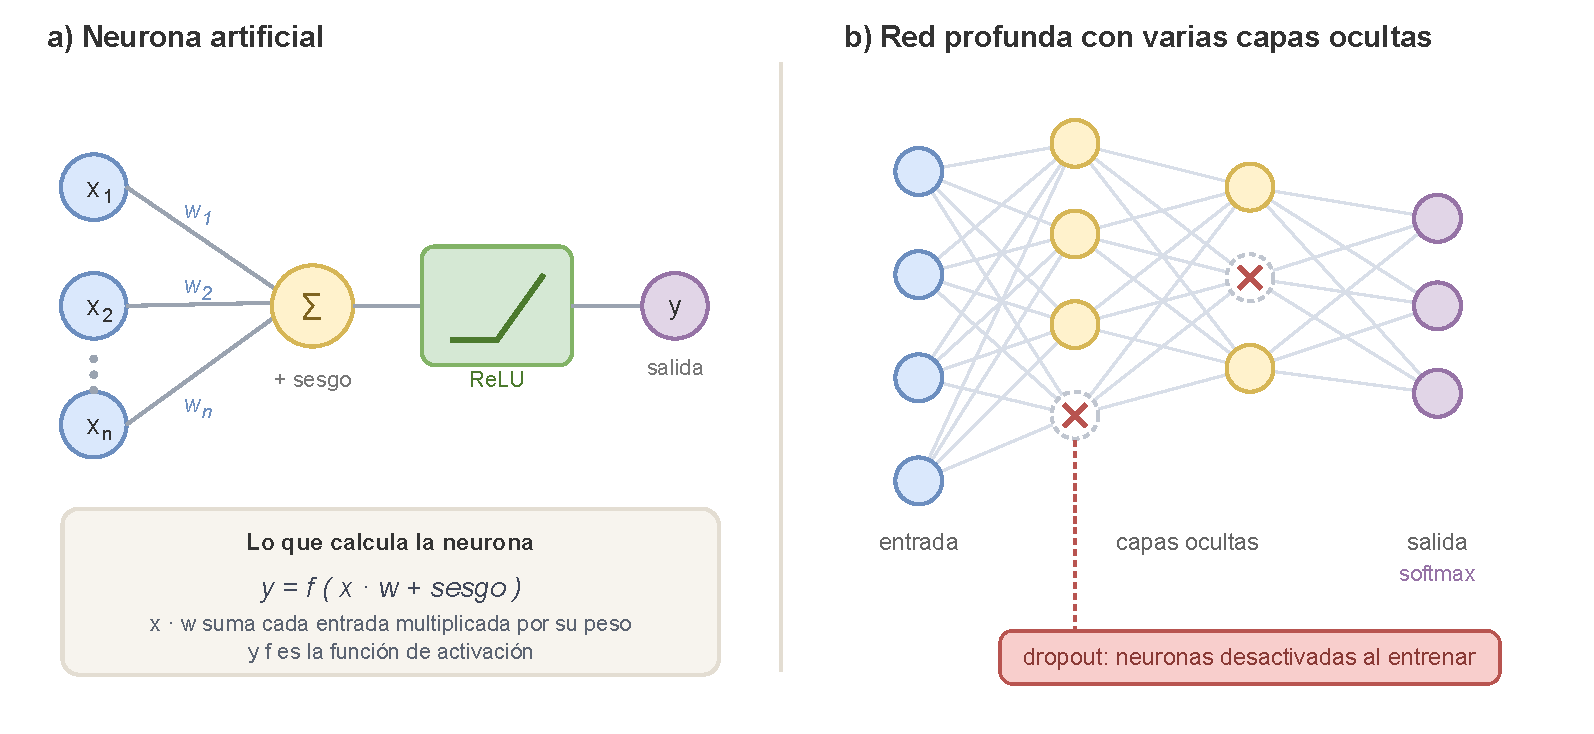
\includegraphics[width=\textwidth]{Figures/Teoria/neurona_red.pdf}
\caption[Neurona artificial y red profunda]{Neurona artificial y red profunda. A la
izquierda, la unidad de cálculo: las entradas se ponderan, se suman junto con el sesgo y
el resultado pasa por una función de activación. A la derecha, la organización en capas,
con la salida softmax y las neuronas que el dropout desactiva durante el entrenamiento.
Fuente: Elaboración propia.}
\label{fig:teoria-neurona}
\end{figure}

Conviene observar en la \autoref{fig:teoria-neurona} que el dropout no elimina neuronas
del modelo: solo las
desactiva de forma temporal y aleatoria en cada paso del entrenamiento, lo que impide que
la red dependa en exceso de unas pocas unidades. En la inferencia, todas vuelven a
participar.

\section{Red Convolucional 1D para la Clasificación del Alfabeto}

El módulo de reconocimiento del alfabeto dactilológico no clasifica un único fotograma,
sino una ventana temporal corta de los últimos 20 fotogramas. Cada fotograma se
representa con un vector de 126 valores, que corresponde a 21 landmarks por mano con
coordenadas $x$, $y$, $z$ para las dos manos. La salida es una de las 33 clases del
sistema: las 30 letras del alfabeto dactilológico del \acrshort{lesho}, incluidos los dígrafos
CH, LL y RR, la clase REPOSO y dos señas de control.

La razón de clasificar una ventana y no un solo fotograma es que cinco letras del
alfabeto, la J, la Ñ, la Z, la LL y la RR, se ejecutan con movimiento, por lo que una
sola pose no las representa. Una ventana de fotogramas captura la trayectoria completa
de estas letras, mientras que una letra estática produce una ventana en la que todos los
fotogramas son casi idénticos. De este modo, una misma arquitectura reconoce tanto las
letras estáticas como las que llevan movimiento.

Para esta tarea se emplea una red neuronal convolucional en una dimensión (\acrshort{cnn} 1D).
Una convolución aplica un filtro que se desliza a lo largo de un eje, en este caso el eje
temporal de la ventana, y detecta patrones locales, como el cambio de forma de la mano
entre fotogramas consecutivos. La red aprende múltiples filtros de este tipo y combina
sus salidas para clasificar la ventana. Frente a una red recurrente, la convolución en
una dimensión es más ligera, se ejecuta de forma paralela y se convierte al formato de
inferencia móvil sin operaciones especiales, lo que la hace idónea para la ejecución en
tiempo real en el dispositivo \cite{goodfellow_deep_2016}, \cite{lecun_deep_2015}.

Antes de alimentar la red, los landmarks de cada fotograma se normalizan en dos pasos.
Primero se resta la coordenada de la muñeca a todos los demás puntos de la misma mano,
de modo que la mano queda centrada en el origen con independencia de su posición en el
encuadre. Luego se divide por el tamaño de la mano, lo que elimina la variación por
distancia de la mano a la cámara. Con esta normalización, la red aprende la configuración
geométrica de la seña y no su posición o escala absoluta en la imagen
\cite{zhang_mediapipe_2020}. El modelo se compone de bloques convolucionales con
activación \acrshort{relu} y agrupación temporal, seguidos de una capa densa con
regularización dropout y una capa de salida softmax de 33 neuronas.

La \autoref{fig:teoria-convolucion} ilustra este funcionamiento sobre la ventana temporal,
junto con la normalización previa de los landmarks.

\begin{figure}[htbp]
\centering
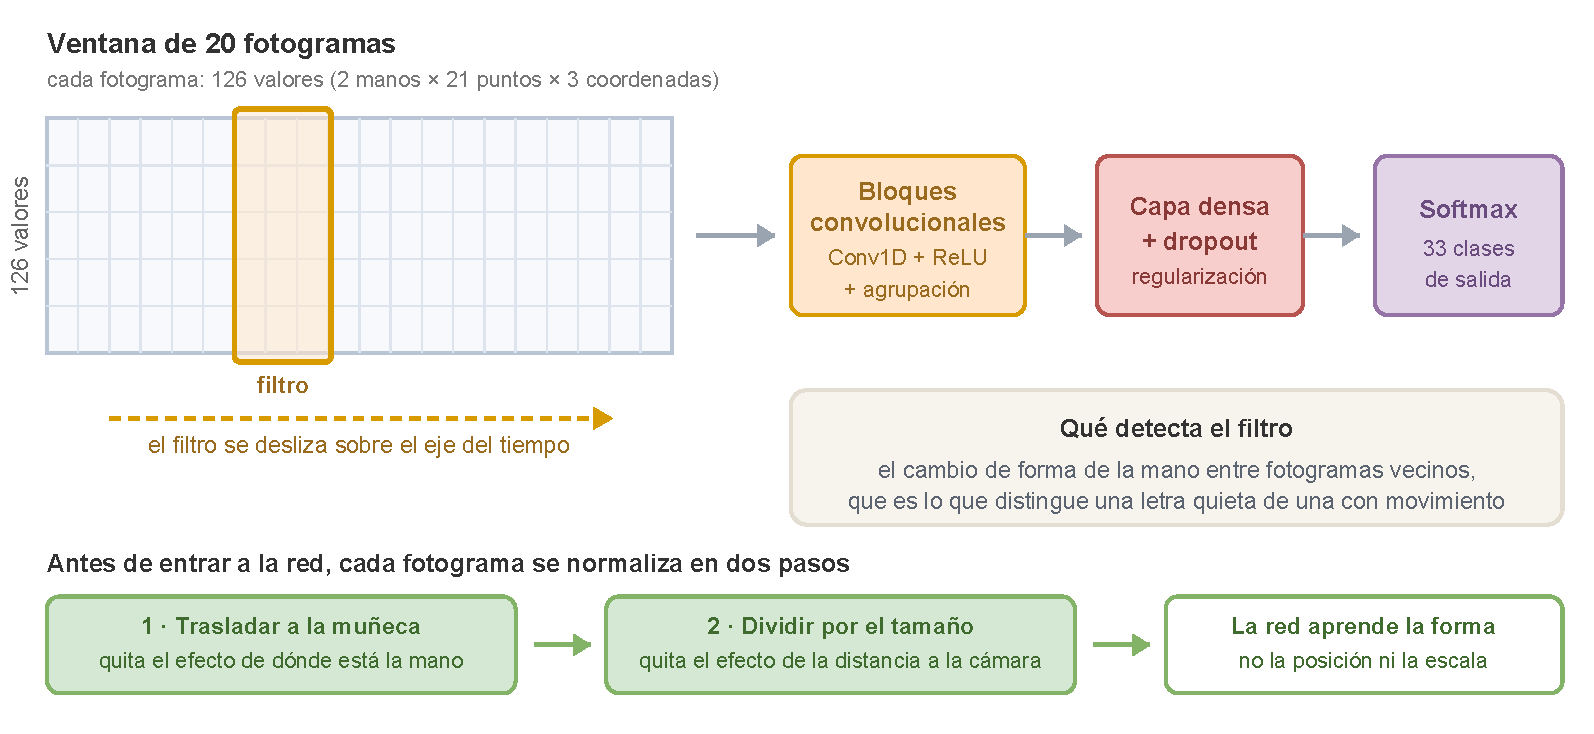
\includegraphics[width=\textwidth]{Figures/Teoria/convolucion_1d.pdf}
\caption[Convolución en una dimensión sobre la ventana temporal]{Convolución en una
dimensión sobre la ventana temporal. El filtro recorre el eje del tiempo y detecta
patrones locales entre fotogramas vecinos; abajo se muestran los dos pasos de
normalización que se aplican a cada fotograma antes de entrar a la red. Fuente:
Elaboración propia.}
\label{fig:teoria-convolucion}
\end{figure}

El detalle que explica la elección de esta arquitectura está en el eje sobre el que se
desliza el filtro. Al recorrer el tiempo y no el espacio de la imagen, la red no compara
formas de mano aisladas sino su evolución entre fotogramas consecutivos, que es
precisamente la información que separa una letra sostenida de una que se ejecuta con
movimiento.

\section{Redes Recurrentes (LSTM y GRU) para Clasificación de Secuencias}

Las señas dinámicas de \acrshort{lesho} involucran movimiento: la mano recorre una trayectoria
en el espacio durante un intervalo de tiempo que puede abarcar varios segundos. A
diferencia de la ventana corta del alfabeto, una seña completa exige modelar dependencias
temporales de mayor alcance, para lo cual conviene una arquitectura con memoria explícita.
Las redes neuronales recurrentes
(\acrshort{rnn}) abordan este problema mediante conexiones cíclicas: la salida en el paso temporal
$t$ depende tanto de la entrada actual como del estado oculto previo, que resume la
información de todos los pasos anteriores. Sin embargo, las \acrshort{rnn} simples sufren el
problema del desvanecimiento del gradiente en secuencias largas, que impide aprender
dependencias a largo plazo \cite{goodfellow_deep_2016}.

La arquitectura Long Short-Term Memory (\acrshort{lstm}), propuesta por Hochreiter y Schmidhuber
en 1997, resuelve este problema mediante tres compuertas multiplicativas
\cite{hochreiter_lstm_1997}. La compuerta de olvido decide qué información del estado
de celda anterior se descarta; la compuerta de entrada controla qué nueva información
se almacena; y la compuerta de salida determina qué parte del estado de celda se expone
como estado oculto. La compuerta de olvido, incorporada por Gers, Schmidhuber y Cummins
en 2000, resulta especialmente relevante para procesar flujos continuos de landmarks de
video \cite{gers_forget_2000}. La unidad recurrente con compuertas (\acrshort{gru}), propuesta por
Cho et al. en 2014, simplifica la arquitectura \acrshort{lstm} al reducir las tres compuertas a
dos, lo que disminuye el número de parámetros sin pérdida significativa de rendimiento
en muchas tareas de secuencias \cite{cho_gru_2014}. Para la clasificación de las 50
señas dinámicas del sistema, se emplea una red \acrshort{lstm} en configuración many-to-one: la
red procesa la secuencia completa de cuadros capturados durante la grabación y
emite una única clasificación al final, tomando el estado oculto del último paso temporal
como entrada a una capa densa de salida softmax. Esta elección se sustenta en la
capacidad demostrada de la \acrshort{lstm} para clasificar secuencias de landmarks de manos en
trabajos previos sobre reconocimiento de lenguas de señas \cite{mittal_lstm_2019},
\cite{khartheesvar_indian_2024}, y en una razón práctica de despliegue: la \acrshort{lstm} cuenta
con una operación fusionada en el marco de inferencia móvil que permite ejecutarla de
forma eficiente en el dispositivo, optimización de la que la \acrshort{gru} no dispone.

La \autoref{fig:teoria-lstm} compara ambas celdas y resume el criterio con que se eligió
una de las dos para este sistema.

\begin{figure}[htbp]
\centering
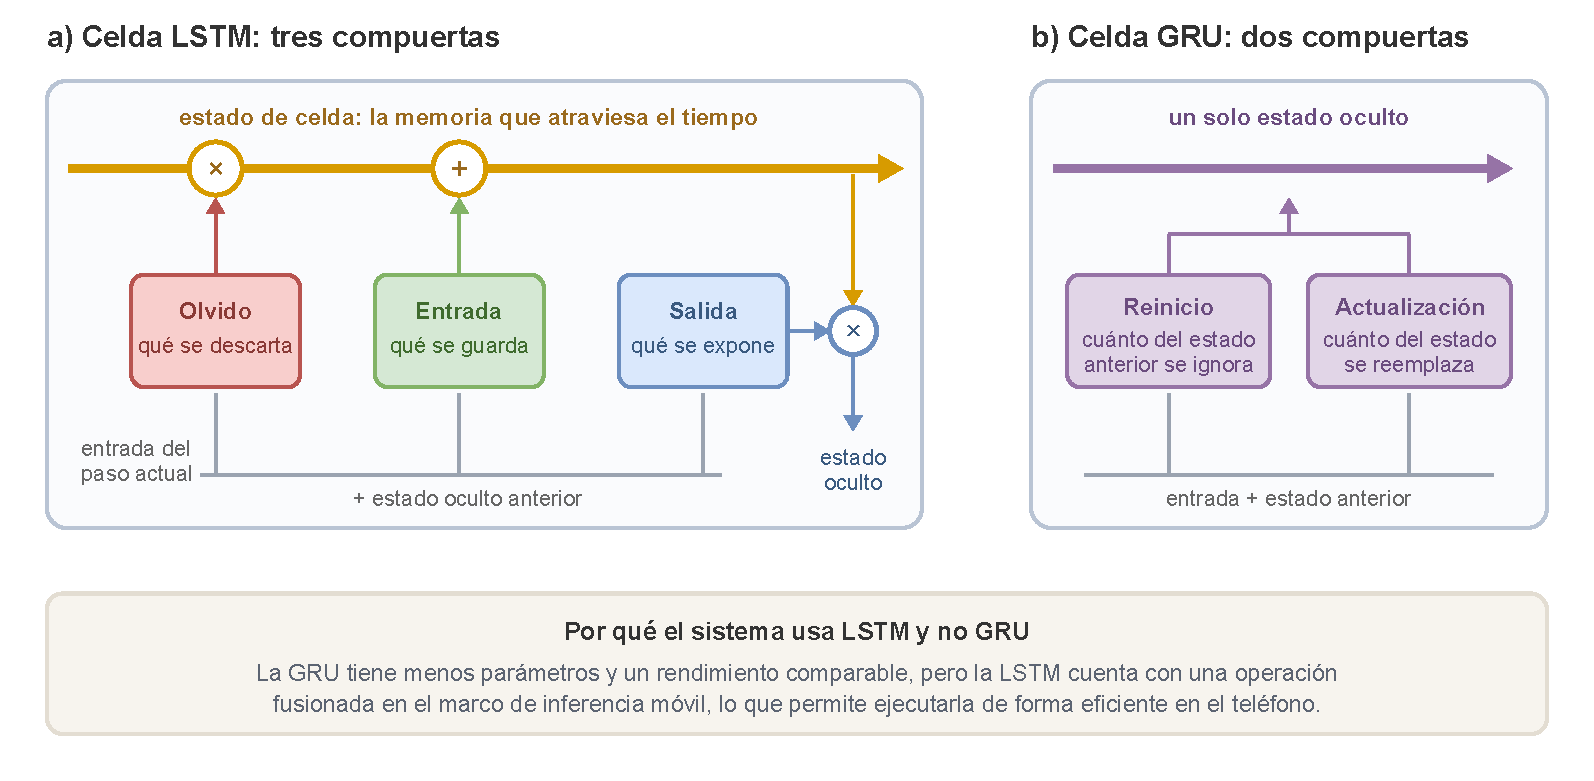
\includegraphics[width=\textwidth]{Figures/Teoria/lstm_gru.pdf}
\caption[Celdas LSTM y GRU]{Esquema simplificado de las celdas \acrshort{lstm} y
\acrshort{gru}. A la izquierda, las tres compuertas de la \acrshort{lstm}: las de olvido y
entrada modifican el estado de celda, que atraviesa la secuencia y funciona como memoria,
mientras que la de salida lo lee para producir el estado oculto. A la derecha, la
\acrshort{gru}, que reduce el mecanismo a dos compuertas sobre un único estado oculto.
Fuente: Elaboración propia.}
\label{fig:teoria-lstm}
\end{figure}

En la \autoref{fig:teoria-lstm} se aprecia por qué la compuerta de olvido resulta
determinante para este
sistema: es la que permite descartar la información de los fotogramas de transición, en
los que la mano viaja entre posiciones sin formar todavía la seña, y conservar en cambio
la del tramo que sí la contiene.

\section{Segmentación Temporal en Flujo Continuo de Gestos}
\label{sec:segmentacion}

En un escenario de uso real, el usuario no realiza señas aisladas frente a la cámara,
sino que produce un flujo continuo de movimientos que incluye señas, transiciones y
movimientos no intencionales. El sistema debe determinar cuándo comienza y cuándo
termina cada seña dentro de este flujo, problema conocido como segmentación temporal,
que representa uno de los desafíos principales del reconocimiento continuo de lengua de
señas \cite{sadik_survey_2025}, \cite{srivastava_continuous_2024}.

El presente sistema adopta una estrategia de segmentación explícita: la persona usuaria
delimita la seña mediante un control en pantalla. Al pulsar el botón de grabación se
activa la captura de la secuencia de landmarks, y al pulsarlo de nuevo la captura se
detiene y la secuencia acumulada se envía al modelo \acrshort{lstm} para su clasificación.
Esta estrategia no requiere modelos adicionales de segmentación ni mecanismos de ventana
deslizante, y funciona con independencia de la duración de la seña.

Durante el desarrollo se evaluó una alternativa que delimitaba la seña con dos gestos de
control reconocidos por el propio modelo del alfabeto, con la intención de que el usuario
no tuviera que tocar la pantalla. Esa alternativa se descartó tras las pruebas en el
dispositivo: varias señas dinámicas del vocabulario juntan las puntas de los dedos con la
mano extendida, una configuración que el modelo confundía con el gesto de cierre, de modo
que la grabación se interrumpía a mitad de la seña. El control explícito en pantalla
resultó más fiable, y el hallazgo se documenta porque delimita una vía que no conviene
seguir sin resolver antes esa ambigüedad.

El deletreo, en cambio, sí opera de forma continua: el modelo del alfabeto clasifica una
ventana tras otra sin que medie ninguna señal de apertura o cierre, de modo que allí el
problema de segmentación persiste. Para evitar clasificaciones inestables causadas por
cuadros de transición, se aplican dos
filtros de postprocesamiento sobre las predicciones del modelo del alfabeto: un filtro de
persistencia temporal que acepta una predicción solo si el modelo produce la misma clase
durante un mínimo de 5 ventanas consecutivas con confianza igual o superior al 60\,\%, y
un período de enfriamiento de 1200 milisegundos tras cada predicción aceptada.

\section{Métricas de Evaluación de Modelos Clasificadores}

Una vez definidas las arquitecturas de los modelos y el mecanismo de segmentación
temporal, es necesario establecer los criterios con los que se medirá su desempeño.

La evaluación de un modelo clasificador parte de la matriz de confusión, una tabla de
$C \times C$ donde $C$ es el número de clases. Cada celda $(i, j)$ contiene el número
de muestras de la clase real $i$ que el modelo clasificó como clase $j$. Los elementos
de la diagonal representan las predicciones correctas, mientras que los elementos fuera
de ella indican errores. Para un sistema de reconocimiento de señas, la matriz de
confusión permite identificar qué señas el modelo confunde con mayor frecuencia,
información especialmente valiosa cuando existen señas visualmente similares
\cite{sokolova_metrics_2009}.

A partir de la matriz de confusión se derivan las métricas estándar. La exactitud
(accuracy) es la proporción de predicciones correctas sobre el total de muestras.
La precisión (precision) de una clase es la proporción de muestras predichas como esa
clase que realmente le pertenecen. La sensibilidad (recall) es la proporción de muestras
de esa clase que el modelo identificó correctamente. La puntuación F1 (F1-score) es la
media armónica de precisión y sensibilidad, útil cuando se busca equilibrar ambas
métricas \cite{sokolova_metrics_2009}. En problemas multiclase con muchas clases, como
los del presente sistema, se utiliza el macro-promedio, que calcula cada métrica de
forma independiente para cada clase y luego promedia los valores, tratando a todas las
clases con igual importancia independientemente de su frecuencia en el conjunto de datos.
Esta elección se justifica porque cada seña de \acrshort{lesho} tiene igual relevancia comunicativa
para el usuario final.

La \autoref{fig:teoria-matriz} muestra un ejemplo con cuatro clases y señala de qué parte
de la matriz se obtiene cada métrica.

\begin{figure}[htbp]
\centering
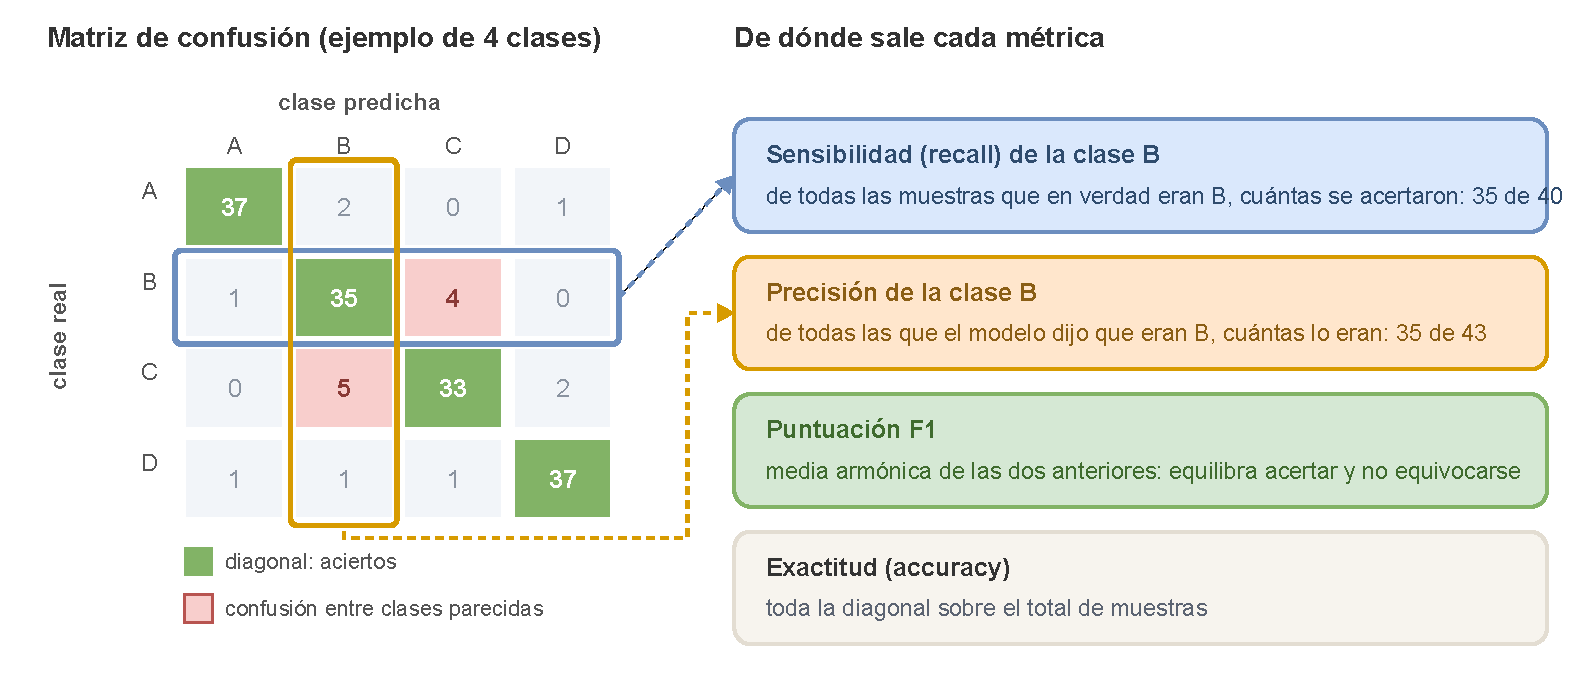
\includegraphics[width=\textwidth]{Figures/Teoria/matriz_confusion.pdf}
\caption[Matriz de confusión y origen de las métricas]{Matriz de confusión de un ejemplo
con cuatro clases. La diagonal concentra los aciertos y las celdas fuera de ella señalan
las confusiones. A la derecha se indica de qué fila o columna se deriva cada métrica.
Fuente: Elaboración propia.}
\label{fig:teoria-matriz}
\end{figure}

La distinción entre la fila y la columna es la que suele prestarse a confusión. La
sensibilidad se lee sobre la fila, porque parte de las muestras que en verdad pertenecen a
la clase; la precisión se lee sobre la columna, porque parte de las que el modelo asignó a
esa clase. Un modelo puede tener sensibilidad alta y precisión baja si acierta casi todas
las muestras de una clase pero además atrae hacia ella muchas de otras.

\section{Inferencia Local en Dispositivos Móviles con TensorFlow Lite}

El diseño del sistema exige que toda la inferencia se ejecute localmente en el teléfono
del usuario, sin enviar datos a un servidor externo. Esta restricción responde a tres
consideraciones: privacidad, disponibilidad en zonas rurales de Honduras sin conexión a
internet, y latencia mínima para que la comunicación sea fluida. TensorFlow Lite (\acrshort{tflite})
es el marco de inferencia de Google diseñado para ejecutar modelos de aprendizaje
automático en dispositivos móviles y con recursos limitados \cite{google_tflite_2024}.
Utiliza un formato de archivo binario basado en FlatBuffer con extensión \texttt{.tflite}
que minimiza el tiempo de carga y la huella de memoria en comparación con el formato
estándar de TensorFlow.

La \autoref{fig:teoria-tflite} resume ese recorrido, desde el modelo entrenado hasta su
ejecución dentro de la aplicación. Los pasos se detallan a continuación.

\begin{figure}[htbp]
\centering
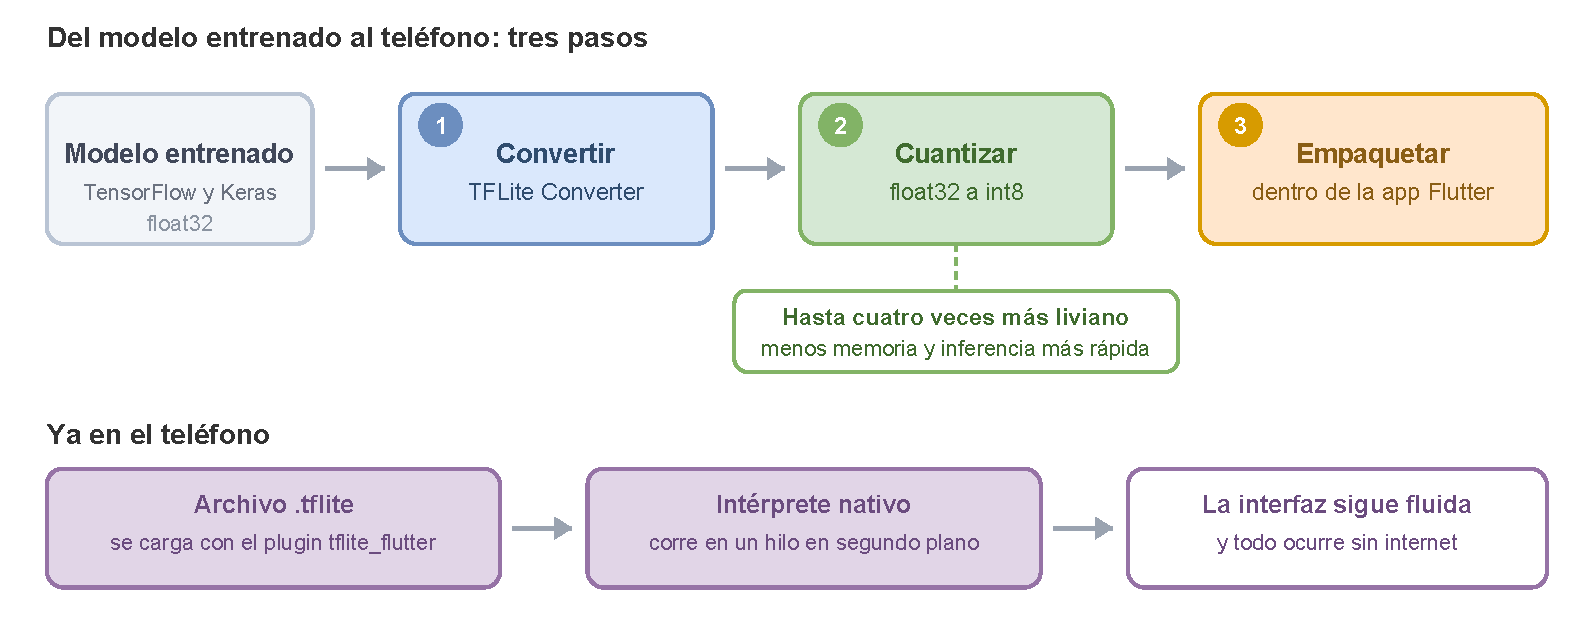
\includegraphics[width=\textwidth]{Figures/Teoria/despliegue_tflite.pdf}
\caption[Flujo de conversión y despliegue con TensorFlow Lite]{Flujo de conversión y
despliegue con \acrshort{tflite}. Arriba, los tres pasos que llevan del modelo entrenado al
archivo empaquetado en la aplicación; abajo, la forma en que ese archivo se carga y se
ejecuta ya en el teléfono. Fuente: Elaboración propia.}
\label{fig:teoria-tflite}
\end{figure}

El flujo de trabajo para desplegar un modelo en el dispositivo consta de tres pasos.
Primero, el modelo entrenado en TensorFlow y Keras se convierte al formato \texttt{.tflite}
mediante el \acrshort{tflite} Converter. Segundo, se aplica cuantización post-entrenamiento para
reducir la precisión numérica de los pesos de punto flotante de 32 bits (float32) a
enteros de 8 bits (int8), lo que reduce el tamaño del modelo hasta cuatro veces,
disminuye el uso de memoria RAM y acelera la inferencia en la CPU del dispositivo
\cite{google_tflite_2024}, \cite{google_quantization_2024}. Tercero, el archivo
\texttt{.tflite} se empaqueta dentro de la aplicación Flutter y se carga mediante el
plugin \texttt{tflite\_flutter}, que proporciona una interfaz en Dart para el intérprete
nativo de \acrshort{tflite} a través de \acrshort{ffi} (Foreign Function Interface). El procesamiento de los cuadros de video se
ejecuta en un hilo nativo en segundo plano, comunicado con la aplicación mediante un canal
de plataforma, lo que garantiza que la interfaz responda con fluidez durante la ejecución
del sistema.
El \autoref{ch:implementacion} detalla la configuración específica de los modelos dentro
de la aplicación, y el \autoref{chap:resultados} reporta el tamaño final de los archivos
convertidos y los tiempos de inferencia medidos en el dispositivo de prueba.

El paso de cuantización es el que hace viable el despliegue en un dispositivo de gama
baja: al reducir la precisión numérica de los pesos, el archivo se aligera de forma
notable y la inferencia se acelera, a cambio de una pérdida de exactitud que en la
práctica resulta mínima para tareas de clasificación como esta.

%\include{Chapters/05-Inteligencia-Artificial}
\chapter{Desarrollo de Aplicaciones Móviles Inclusivas}
\label{cp:aplicaciones-moviles}

\insertminitoc
\parindent0pt

Una aplicación de reconocimiento de lengua de señas para niños sordos no es únicamente
un proyecto de inteligencia artificial; es, ante todo, un producto de software que debe
funcionar con fiabilidad en un dispositivo móvil, procesar video en tiempo real, presentar
una interfaz comprensible para un público infantil y enmarcarse dentro del campo de la
comunicación aumentativa y alternativa. El presente capítulo aborda estos cuatro ejes: el
framework de desarrollo multiplataforma utilizado, la integración de modelos de
inteligencia artificial con la cámara del dispositivo, los principios de diseño de
interfaces accesibles para niños y el marco conceptual de las tecnologías de comunicación
aumentativa y alternativa (\acrshort{caa}) en el que se inserta el sistema.

\section{Desarrollo Móvil Multiplataforma con Flutter}

Flutter es un framework de código abierto desarrollado por Google para la construcción de
aplicaciones compiladas de forma nativa a partir de una base de código única en el lenguaje
Dart \cite{google_flutter_2024}. A diferencia de otros frameworks multiplataforma que
dependen de un puente de comunicación con los componentes nativos del sistema operativo,
Flutter compila el código Dart de forma anticipada (ahead-of-time, \acrshort{aot}) a código de
máquina nativo y utiliza su propio motor de renderizado gráfico para dibujar cada píxel de
la interfaz, lo que produce un rendimiento cercano al de una aplicación nativa
\cite{google_flutter_2024}.

La arquitectura de Flutter se organiza en capas. La capa inferior es el motor (engine),
escrito en C++, que se encarga del renderizado gráfico, la composición, la gestión de
entrada y salida y la comunicación con el sistema operativo. Sobre esta capa se encuentra
el framework en Dart, que proporciona un sistema de widgets reactivos con el cual se
construye toda la interfaz de usuario. Cada elemento visual, desde un botón hasta la
distribución de la pantalla, es un widget que se combina de forma declarativa con otros
widgets para formar interfaces complejas \cite{google_flutter_2024}. Este modelo
declarativo facilita la construcción de interfaces dinámicas que se actualizan en respuesta
a cambios de estado, lo que resulta especialmente útil para una aplicación que muestra
resultados de clasificación en tiempo real. Flutter permite generar aplicaciones para
Android e iOS desde el mismo código, lo cual reduce el esfuerzo de desarrollo y
mantenimiento del sistema.

\section{Integración de Modelos de Inteligencia Artificial y Procesamiento de Cámara en Tiempo Real}

El sistema propuesto requiere que la cámara frontal del dispositivo capture cuadros de
video de forma continua, que MediaPipe Hands y MediaPipe Pose extraigan los landmarks de
las manos y del cuerpo en cada cuadro, y que los modelos descritos en el capítulo 6, la
red convolucional 1D para el alfabeto y la red \acrshort{lstm} para las señas dinámicas, clasifiquen
los gestos detectados. Todo este procesamiento debe ocurrir en tiempo real, sin bloquear
la interfaz de usuario y sin enviar datos a un servidor externo.

En Flutter, el acceso a la cámara se gestiona a través del plugin camera, que proporciona
un flujo de cuadros (stream) desde la cámara del dispositivo. Cada cuadro se transfiere
como un arreglo de bytes al canal de procesamiento de MediaPipe Hands, que devuelve las
coordenadas de los 21 landmarks por mano detectada \cite{google_mediapipe_2024},
\cite{zhang_mediapipe_2020}. Estos landmarks se normalizan y se pasan al intérprete de
TensorFlow Lite para obtener la predicción del modelo \cite{google_tflite_2024}. Para
evitar que este procesamiento bloquee el hilo principal de la interfaz, la extracción de
landmarks con MediaPipe se ejecuta en un hilo nativo en segundo plano, comunicado con
Flutter mediante un canal de plataforma, de modo que el hilo de la interfaz permanece libre. Sousa et al. validaron la viabilidad de esta arquitectura en un
sistema de reconocimiento de Lengua de Señas Portuguesa implementado con Flutter,
MediaPipe y \acrshort{tflite}, donde reportaron tiempos de inferencia compatibles con una
experiencia de uso fluida en dispositivos Android de gama media \cite{sousa_lgp_flutter_2025}.

\section{Diseño de Interfaces para Niños y Accesibilidad}

El público objetivo del sistema es la población infantil sorda, lo que impone restricciones
de diseño particulares. Hourcade señala que las interfaces dirigidas a niños deben
minimizar el uso de texto, privilegiar representaciones visuales e iconográficas, utilizar
elementos de interacción de tamaño suficiente para las habilidades motoras en desarrollo y
ofrecer retroalimentación inmediata ante cada acción del usuario \cite{hourcade_children_2008}.
En el caso de niños sordos, estas consideraciones se intensifican: la lengua escrita suele
ser una segunda lengua adquirida con dificultad, por lo que la interfaz debe apoyarse en
recursos visuales como colores, iconos y animaciones para comunicar el estado del sistema
y los resultados de la clasificación.

Las directrices de accesibilidad de contenido web \acrshort{wcag} 2.1, publicadas por el \acrshort{w3c} en
2018, establecen cuatro principios fundamentales: el contenido debe ser perceptible,
operable, comprensible y robusto \cite{w3c_wcag_2018}. Si bien estas directrices fueron
concebidas para contenido web, sus principios son aplicables al diseño de interfaces
móviles. En particular, el principio de perceptibilidad exige que la información se
presente de formas que el usuario pueda percibir, lo que para un usuario sordo implica que
toda la retroalimentación del sistema debe ser visual o háptica, nunca exclusivamente
auditiva. Flutter proporciona soporte nativo para herramientas de accesibilidad del sistema
operativo como TalkBack (Android) y VoiceOver (iOS), y permite configurar etiquetas
semánticas en los widgets para que los lectores de pantalla describan correctamente cada
elemento de la interfaz \cite{google_flutter_2024}. La Convención sobre los Derechos de
las Personas con Discapacidad de las Naciones Unidas refuerza este enfoque al establecer
que las tecnologías de la información deben ser accesibles y estar disponibles para las
personas con discapacidad en igualdad de condiciones \cite{onu_cdpd_2006}.

\section{Tecnologías de Comunicación Aumentativa y Alternativa}

El sistema desarrollado no es únicamente una aplicación móvil con modelos de inteligencia
artificial; desde el punto de vista comunicativo, se enmarca dentro de un campo más amplio
con una tradición consolidada de herramientas diseñadas para apoyar la comunicación de
personas que no pueden depender exclusivamente del habla oral.

La comunicación aumentativa y alternativa (\acrshort{caa}) es un término general que abarca todos
los métodos de comunicación distintos al habla oral que permiten a las personas expresar
pensamientos, necesidades y sentimientos. La American Speech-Language-Hearing Association
(\acrshort{asha}) define la \acrshort{caa} como un conjunto de herramientas y estrategias que incluye tableros
de imágenes, dispositivos generadores de habla, signos manuales, gestos y deletreo con los
dedos \cite{asha_aac_nodate}. Los sistemas de \acrshort{caa} se clasifican en dos categorías: los
sistemas sin ayuda (unaided), que utilizan únicamente el cuerpo del usuario, como las
lenguas de señas y los gestos, y los sistemas con ayuda (aided), que requieren un
dispositivo externo, desde un tablero de imágenes impreso hasta una aplicación en un
teléfono inteligente \cite{beukelman_aac_2020}.

Beukelman y Light clasifican los sistemas con ayuda según su nivel tecnológico: sin
tecnología (tableros de papel), baja tecnología (dispositivos con botones y mensajes
pregrabados) y alta tecnología (software con generación de habla, predicción de texto y
acceso a vocabulario extenso) \cite{beukelman_aac_2020}. La aplicación desarrollada en
el presente proyecto se ubica en esta última categoría, con la particularidad de que
integra visión por computadora para interpretar los gestos del usuario en lugar de
depender de la selección manual de símbolos en pantalla. La combinación de un módulo de
reconocimiento de señas (dirección niño a oyente) con un diccionario visual de señas
(dirección oyente a niño) convierte al sistema en una herramienta de
comunicación bidireccional que abarca tanto la función aumentativa como la alternativa de
la \acrshort{caa}, adaptada específicamente a las necesidades de la comunidad sorda hondureña y a la
Lengua de Señas Hondureña (\acrshort{lesho}).

\include{Chapters/Marco-Conceptual}
\chapter[Marco Legal]{Marco Legal}
\label{ch:marco-legal}

\insertminitoc
\parindent0pt

El desarrollo de una aplicación de reconocimiento de lengua de señas para niños sordos se
enmarca en un conjunto de disposiciones jurídicas que protegen los derechos de las personas
con discapacidad y promueven su inclusión educativa y comunicativa. Este capítulo presenta
los instrumentos legales internacionales y nacionales que fundamentan y legitiman el
presente proyecto, así como los estándares técnicos de accesibilidad que orientan el diseño
del sistema.

\section{Derecho a la Comunicación y Educación Inclusiva en el Marco Internacional}

La Convención sobre los Derechos de las Personas con Discapacidad (\acrshort{cdpd}), adoptada por la
Asamblea General de las Naciones Unidas en 2006 y ratificada por Honduras, establece en su
artículo 9 la obligación de los Estados de asegurar el acceso de las personas con
discapacidad a la información y las comunicaciones, incluidas las tecnologías de la
información. El artículo 21 reconoce el derecho a la libertad de expresión mediante las
lenguas de señas y otros modos y formatos de comunicación accesibles, mientras que el
artículo 24 exige que los Estados garanticen una educación inclusiva a todos los niveles,
facilitando el aprendizaje de la lengua de señas y promoviendo la identidad lingüística de
las personas sordas \cite{onu_cdpd_2006}.

La Agenda 2030 para el Desarrollo Sostenible, aprobada por las Naciones Unidas en 2015,
incorpora la discapacidad como eje transversal en sus metas. El Objetivo de Desarrollo
Sostenible 4 (Educación de Calidad) establece el compromiso de garantizar una educación
inclusiva, equitativa y de calidad para todas las personas. El Objetivo 10 (Reducción de
las Desigualdades) promueve la inclusión social y económica de las personas con
discapacidad independientemente de su condición \cite{onu_agenda2030_2015}. El presente
proyecto contribuye directamente a ambos objetivos al proporcionar una herramienta
tecnológica que facilita la comunicación entre niños sordos y personas oyentes en contextos
educativos.

La Declaración de Salamanca, adoptada por la UNESCO en 1994, constituye un referente
fundamental en materia de educación inclusiva. Este instrumento proclama que los sistemas
educativos deben diseñarse para atender la diversidad de necesidades de aprendizaje, y que
los niños con necesidades educativas especiales deben tener acceso a las escuelas ordinarias
como medio más eficaz para combatir actitudes discriminatorias y construir una sociedad
inclusiva \cite{unesco_salamanca_1994}.

\section{Legislación Hondureña en Materia de Discapacidad y Lengua de Señas}

La Constitución de la República de Honduras, en su artículo 60, declara punible toda
discriminación. El artículo 151 establece que la educación es función esencial del Estado,
y el artículo 169 dispone que el Estado sostendrá y fomentará la educación de las personas
con discapacidad \cite{constitucion_honduras_1982}. Estas disposiciones constitucionales
proporcionan el fundamento jurídico superior sobre el cual se apoyan las leyes específicas
en materia de discapacidad.

La Ley de Equidad y Desarrollo Integral para las Personas con Discapacidad (Decreto
160-2005) tiene como finalidad garantizar el disfrute pleno de los derechos de las personas
con discapacidad y promover su desarrollo integral dentro de la sociedad. Esta ley prohíbe
toda forma de discriminación directa o indirecta, establece principios de autodeterminación
y accesibilidad universal, y obliga a los órganos rectores de educación a asegurar el
acceso efectivo de las personas con discapacidad al sistema educativo \cite{decreto_160_2005}.
En su artículo 12, la ley establece que los medios de comunicación deben facilitar el
acceso a la información para las personas con discapacidad, lo que respalda el desarrollo
de herramientas tecnológicas como la que propone este proyecto.

La Ley de la Lengua de Señas Hondureña (Decreto 321-2013) reconoce al \acrshort{lesho} como medio de
comunicación oficial en el territorio nacional para las personas sordas, con discapacidad
auditiva y sordociegas, y establece la obligación del Estado de
promover su uso, enseñanza y difusión en todos los ámbitos sociales y educativos
\cite{congreso_decreto_2013}. Esta ley es de particular relevancia para el presente
proyecto, ya que legitima el desarrollo de tecnologías orientadas al reconocimiento y la
difusión de \acrshort{lesho} como instrumento de comunicación y de acceso a la educación para la
comunidad sorda hondureña.

\section{Normativa Técnica de Accesibilidad Aplicable al Sistema}

Las Pautas de Accesibilidad para el Contenido Web (\acrshort{wcag}) 2.1, publicadas por el World Wide
Web Consortium (\acrshort{w3c}) en 2018, constituyen el estándar internacional de referencia para el
diseño de contenido digital accesible. Aunque fueron concebidas para contenido web, sus
cuatro principios (perceptible, operable, comprensible y robusto) son aplicables al diseño
de aplicaciones móviles \cite{w3c_wcag_2018}. Para el presente sistema, el principio de
perceptibilidad resulta determinante: toda retroalimentación del sistema debe ser visual o
háptica, dado que el usuario principal es un niño sordo. Los criterios de contraste de
color, tamaño de elementos interactivos y alternativas textuales para contenido no textual
orientan directamente las decisiones de diseño de la interfaz de la aplicación.

\section{Protección de los Datos de las Personas Participantes}

El sistema propuesto capta imágenes de personas mediante la cámara del dispositivo, y su
construcción exigió grabar a colaboradores ejecutando señas. Ambas circunstancias sitúan
al proyecto en el terreno de la protección de datos personales, por lo que corresponde
precisar el marco jurídico aplicable en Honduras.

A la fecha de este trabajo, Honduras no cuenta con una ley integral de protección de datos
personales en vigor. Existe un anteproyecto que ha sido presentado ante el Congreso
Nacional, pero no ha completado su trámite legislativo. En ausencia de esa norma
específica, la protección se sustenta en el texto constitucional.

La Constitución de la República de Honduras, en su artículo 76, garantiza el derecho al
honor, a la intimidad personal y familiar y a la propia imagen. El artículo 100 establece
la inviolabilidad y el secreto de las comunicaciones. Y el artículo 182, en su numeral
segundo, reconoce la garantía de hábeas data, que otorga a toda persona un recurso para
conocer y controlar la información que sobre ella conste en registros o bancos de datos
\cite{constitucion_honduras_1982}. El derecho a la propia imagen es el que incide de forma
más directa en este proyecto, tanto por la captación de video durante la construcción del
conjunto de datos como por el uso de la cámara en la aplicación.

Frente a ese marco, el diseño del sistema adopta dos garantías técnicas que van más allá
de lo que exigiría una norma. La primera es que los videos no se almacenan en ningún
momento: cada fotograma se procesa para extraer las coordenadas de los puntos anatómicos y
la imagen se descarta, de modo que el conjunto de datos está compuesto únicamente por
valores numéricos a partir de los cuales no es posible reconstruir el rostro ni la
apariencia de una persona. La segunda es que todo el procesamiento ocurre en el propio
dispositivo, sin que ninguna imagen se transmita a servidores externos.

La participación de los colaboradores se documenta mediante una hoja de información y un
consentimiento informado, elaborados conforme a los principios éticos internacionales
aplicables a la investigación con seres humanos. El consentimiento distingue de forma separada la participación en el estudio, la
publicación del conjunto de datos bajo seudónimo y el uso de fotografías de las sesiones,
de manera que cada persona pueda autorizar unas y no otras.

La aplicación de estos marcos jurídicos y estándares técnicos asegura que el sistema
propuesto no solo responde a una necesidad tecnológica, sino que se alinea con las
obligaciones del Estado hondureño en materia de inclusión educativa, con los compromisos
internacionales adquiridos por el país y con las mejores prácticas de accesibilidad
digital.


%%% Part 3: Marco Metodológico %%%
\cleardoublepage
\thispagestyle{empty} % Sin encabezado, sin pie de página

% === Registrar la parte en el índice ===
\refstepcounter{part} % Incrementa el contador de partes
\addcontentsline{toc}{part}{Parte \thepart: Marco Metodológico}

% === Fondo decorativo ===
\AddToShipoutPictureBG*{%
	\put(0,0){%
		\parbox[b][\paperheight]{\paperwidth}{%
			\vfill
			\centering
			
\includegraphics[width=\paperwidth,height=\paperheight]{Figures/Theme/Front-Page-E.pdf}%
			\vfill
		}%
	}%
}

% === Contenido de la portada de parte ===
\vspace*{\fill}
\begin{center}
	{\Huge\bfseries Parte \thepart}\\[2cm]
	{\Huge\bfseries MARCO METODOLÓGICO}
\end{center}
\vspace*{\fill}

\clearpage

\chapter[Marco Metodológico]{Marco Metodológico}
\label{ch:metodologia}

\insertminitoc
\parindent0pt

El marco teórico desarrollado en los capítulos anteriores establece las bases conceptuales,
técnicas y normativas que sustentan el sistema propuesto. El presente capítulo describe
la metodología que se adoptará para su construcción y evaluación: el tipo y diseño de
investigación, los actores involucrados, las técnicas e instrumentos que se utilizarán para la
recolección y el procesamiento de los datos, el procedimiento que se seguirá a lo largo del
desarrollo y los métodos de validación que se emplearán.

\section{Tipo de investigación}

Por su propósito, la investigación se clasifica como aplicada \cite{sampieri_metodologia_2014}.
Su objetivo central no es generar conocimiento teórico nuevo, sino construir una
herramienta tecnológica funcional que resuelve un problema concreto: la brecha de
comunicación entre niños sordos, cuya lengua materna es el \acrshort{lesho}, y personas
oyentes que no conocen esa lengua. El punto de partida son conocimientos ya establecidos
en disciplinas como la visión por computadora, el aprendizaje profundo y el desarrollo
de aplicaciones móviles, que se combinan y adaptan para producir un sistema funcional
que facilita la comunicación entre ambas poblaciones en distintos contextos de la vida
cotidiana.

El enfoque adoptado es mixto \cite{sampieri_metodologia_2014}. La componente cuantitativa
abarca la construcción del conjunto de datos de landmarks, el entrenamiento y la
evaluación de los modelos de clasificación mediante métricas estándar como exactitud,
precisión, sensibilidad y puntuación F1, y la medición del tamaño de los modelos
exportados y los tiempos de inferencia en dispositivos reales. La componente cualitativa
corresponde a las sesiones de validación con usuarios de la Fundación CasAyuda,
donde se observa la interacción de los
participantes con la aplicación y se recopila retroalimentación sobre la comprensión de
la interfaz, la facilidad de uso y la adecuación de las señas reconocidas. Ambas
componentes se complementan: las métricas cuantitativas miden el desempeño técnico del
sistema, mientras que la observación cualitativa evalúa su pertinencia y usabilidad en
el contexto real para el que será diseñado.

El alcance de la investigación es exploratorio-descriptivo \cite{sampieri_metodologia_2014}.
Es exploratorio porque, al momento de realizar el estudio, no existen antecedentes
documentados de sistemas de reconocimiento automático de señas del \acrshort{lesho} entrenados
con técnicas de aprendizaje profundo, ni conjuntos de datos de landmarks de la lengua
disponibles públicamente. En ese sentido, la investigación abre un camino metodológico
en un dominio no explorado previamente en Honduras. Es descriptivo porque documenta de
forma sistemática el diseño del sistema, la arquitectura de los modelos, el proceso de
construcción del conjunto de datos y el comportamiento del sistema medido a través de
métricas reproducibles.

El diseño es no experimental \cite{sampieri_metodologia_2014}. No se conformará un grupo
de control ni se manipularán variables de forma aleatoria. El proceso seguirá un diseño de
investigación de desarrollo tecnológico: se definirán los requisitos del sistema, se
construirá el conjunto de datos, se entrenarán y validarán los modelos, se integrarán en una
aplicación móvil y se realizarán pruebas con usuarios reales. Este diseño es coherente con
la naturaleza del problema, donde el objetivo es demostrar la viabilidad técnica de una
solución antes de escalarla a un vocabulario más amplio o a condiciones de uso más
diversas.

\section{Diseño Metodológico}

La investigación se estructuró en cuatro fases secuenciales. La primera consistió en la
consulta con personas con conocimiento del \acrshort{lesho} para definir el vocabulario que el
sistema reconoce y muestra. La segunda comprendió la construcción del conjunto de datos
de landmarks mediante sesiones de grabación con cuatro participantes. La tercera abarcó
el entrenamiento de los modelos de clasificación y su integración en la aplicación móvil.
La cuarta fase corresponde a la validación del sistema con usuarios de la Fundación
CasAyuda. Cada fase produce entregables concretos que sirven como insumo para la
siguiente.

Una decisión metodológica transversal a todas las fases es el procesamiento
completamente local en el dispositivo. Esta decisión implica que ningún dato de cámara
se transmita a servidores externos, ni durante el uso de la aplicación ni durante la
captura del conjunto de datos. Los frames de video se procesarán en tiempo real con
MediaPipe Hands para extraer coordenadas de landmarks, y solo esas coordenadas se
almacenarán de forma permanente. Los videos crudos no se conservarán. Esta restricción,
motivada por consideraciones de privacidad, disponibilidad sin conexión a internet y
minimización de costos de infraestructura, condiciona las decisiones de diseño tanto del
script de captura de datos como de la arquitectura de la aplicación.

La elección de representar las señas mediante vectores de landmarks en lugar de imágenes
de video también responde a razones metodológicas. Al reducir cada mano a 21 puntos con
tres coordenadas, la entrada de los modelos es invariante ante variaciones de
iluminación, tono de piel y fondo, lo que hace que el conjunto de datos sea más
generalizable a distintas condiciones de uso, dispositivos y entornos de grabación.

\section{Población y Muestra}

\subsection{Población}

La población de esta investigación comprende tres grupos de personas involucrados en
situaciones de comunicación mediada por el \acrshort{lesho} en Honduras: niños y jóvenes
sordos que utilizan el \acrshort{lesho} como lengua materna, personas oyentes que interactúan
con ellos en contextos cotidianos, y personas con dominio del \acrshort{lesho} que participarán
como colaboradoras en la construcción del conjunto de datos y en la validación del
sistema. Estos tres grupos constituyen el universo de personas directamente implicadas
en el problema de comunicación que la aplicación busca atender.

\subsection{Muestra}

La muestra estará constituida por 30 personas seleccionadas mediante muestreo no
probabilístico intencional \cite{sampieri_metodologia_2014}. Este tipo de muestreo es
adecuado para investigaciones de carácter aplicado en las que no existe un marco
muestral que permita selección aleatoria y cuyo objetivo no es la generalización
estadística, sino la validación de un sistema funcional con participantes que cumplen
criterios específicos de inclusión.

El número de 30 participantes responde a tres criterios concurrentes. El primero es la
necesidad de representar los tres perfiles involucrados en el problema de comunicación:
personas sordas, personas con dominio del \acrshort{lesho} y personas oyentes. Sin presencia de
los tres grupos no sería posible evaluar ambas direcciones de comunicación del sistema
ni recopilar retroalimentación desde todas las perspectivas relevantes. El segundo
criterio es la suficiencia para el análisis descriptivo de los resultados del
cuestionario aplicado en la etapa de validación: muestras de esta magnitud permiten
calcular frecuencias, porcentajes y medidas de tendencia central de forma interpretable
sin requerir técnicas de inferencia estadística. El tercer criterio es la viabilidad
de acceso: la población de personas con dominio del \acrshort{lesho} en Honduras con afiliación
institucional verificable es reducida y está concentrada en organizaciones especializadas
como la Fundación CasAyuda, lo que limita de forma real el tamaño de muestra
alcanzable con garantías de idoneidad.

Los participantes se distribuirán en tres grupos según su función en la investigación:

\begin{itemize}
    \item \textbf{Personas sordas:} usuarios del módulo de reconocimiento de señas.
    Interactuarán con la aplicación ejecutando señas frente a la cámara y evaluarán la
    respuesta del sistema y la claridad de la interfaz.
    \item \textbf{Personas con dominio del \acrshort{lesho}:} participarán en la construcción del
    conjunto de datos ejecutando el vocabulario definido frente a la cámara, y también en
    las sesiones de validación evaluando la adecuación de las señas reconocidas y mostradas
    por el sistema.
    \item \textbf{Personas oyentes:} usuarios del módulo de texto a seña. Escribirán frases
    en español y evaluarán la representación visual generada por el sistema.
\end{itemize}

Los criterios de inclusión serán los siguientes: para el primer grupo, ser persona
sorda con uso activo del \acrshort{lesho}; para el segundo, tener dominio reconocido de la
lengua; para el tercero, ser persona oyente sin conocimiento previo del \acrshort{lesho}. No se
establecerá restricción por edad, género ni nivel de escolaridad, dado que la aplicación
se diseñará para entornos de uso variados.

\section{Técnicas e Instrumentos de Recolección de Datos}

La recolección de datos abarcará dos procesos diferenciados: la construcción del conjunto
de datos de landmarks para el entrenamiento de los modelos, y la validación del sistema
con usuarios reales. Cada proceso empleará técnicas e instrumentos distintos según sus
objetivos.

Para la construcción del conjunto de datos se utilizará la técnica de grabación controlada
de señas. Cada participante se ubicará frente a la cámara del dispositivo a una distancia
de entre 60 y 100 centímetros, con iluminación natural o interior estándar. El
instrumento principal será un script de captura desarrollado en Python que automatizará
todo el proceso: mostrará en pantalla la seña a ejecutar junto con una imagen de
referencia, presentará una cuenta regresiva de tres segundos, registrará la ejecución
durante dos a tres segundos y avanzará automáticamente a la siguiente seña sin
intervención manual. MediaPipe Hands se integrará directamente en
el script para extraer, en tiempo real, las coordenadas tridimensionales de los 21
landmarks de la mano detectada por cada frame. Dichas coordenadas se normalizarán
restando la posición de la muñeca a todos los demás puntos y se almacenarán en archivos
CSV etiquetados por clase. Los videos no se conservarán.

Para la validación del sistema con usuarios de la Fundación CasAyuda se
aplicará un cuestionario. El instrumento recogerá la percepción de los participantes
sobre la comprensión de la interfaz, la facilidad de interacción con la aplicación y la
adecuación de las señas reconocidas y mostradas por el sistema. Las respuestas
permitirán identificar aspectos de la experiencia de uso que no son evidentes a partir
de las métricas técnicas de los modelos.

\section{Procedimiento}

El desarrollo del sistema seguirá cinco fases secuenciales. Cada una producirá entregables
concretos que servirán como insumo para la siguiente etapa.

\subsection{Definición del vocabulario}

La primera fase consistirá en establecer con precisión las señas que el sistema
reconocerá y mostrará. En coordinación con personas con conocimiento del \acrshort{lesho}
vinculadas a la Fundación CasAyuda, se seleccionarán las 50 señas
dinámicas que conformarán el vocabulario del Modelo B. Los criterios de selección
priorizarán señas de uso cotidiano para niños, representativas de categorías como
emociones, familia, necesidades básicas, números y colores. En la misma etapa se definirán
dos señas de control, concebidas inicialmente para delimitar el inicio y el final de una
seña dinámica sin tocar la pantalla, que deberán ser visualmente distintas entre sí y de
cualquier letra del alfabeto dactilológico. Las 30 letras del alfabeto dactilológico,
incluidos los dígrafos CH, LL y RR, completarán el vocabulario del alfabeto, junto con una
clase de reposo. Al concluir esta fase, el vocabulario total del sistema quedará cerrado:
33 clases para el Modelo A y 50 señas dinámicas para el Modelo B.

\subsection{Construcción del conjunto de datos}

Con el vocabulario definido se realizaron las sesiones de grabación con cuatro
participantes, utilizando el script de captura descrito en la sección anterior.

El conjunto de datos del Modelo A abarca las 33 clases: las 30 letras del alfabeto
dactilológico, la clase REPOSO y las dos señas de control. Cada participante grabó 20
tomas de cada clase estática y 40 tomas de cada una de las cinco letras que se ejecutan con
movimiento (J, Ñ, Z, LL y RR), cuya trayectoria requiere más ejemplos. De cada toma se
extraen ventanas de 20 fotogramas, que constituyen la entrada del modelo; cada fotograma se
representa con 126 valores, correspondientes a las coordenadas $x$, $y$ y $z$ de los 21
landmarks de las dos manos, normalizadas respecto a la posición de la muñeca.

Para el conjunto de datos del Modelo B, cada participante grabó 25 tomas de cada una de
las 50 señas dinámicas, lo que conformó un total de 5\,000 secuencias con los
cuatro participantes. Cada secuencia comprende entre 30 y 60 fotogramas según la duración
natural de la seña, que se remuestrean a una longitud fija de 40. A diferencia del Modelo A,
cada fotograma del Modelo B combina la configuración de las manos (126 valores) con la
ubicación de estas respecto al cuerpo, obtenida con MediaPipe Pose (18 valores); con los
rasgos relativos que se derivan en el preprocesamiento, la entrada final al modelo es de 152
valores. Ambos conjuntos se almacenarán en formato CSV sin incluir video crudo. Como técnicas de aumento de datos se aplicarán variación de velocidad
mediante submuestreo y sobremuestreo temporal, y ruido gaussiano leve sobre las
coordenadas de los landmarks para simular la variación natural en la ejecución de cada
seña.

\subsection{Entrenamiento y exportación de los modelos}

Los conjuntos de datos se dividirán en subconjuntos de entrenamiento y evaluación para
el ajuste y validación de cada modelo.

El Modelo A se implementará como una red neuronal convolucional en una dimensión
(\acrshort{cnn} 1D) sobre el eje temporal de la ventana, con activación \acrshort{relu} y regularización
mediante dropout. La capa de salida utiliza la función softmax sobre 33 neuronas. El modelo se entrenará con el optimizador Adam y la
función de pérdida de entropía cruzada categórica, con detención temprana sobre el
conjunto de validación para prevenir el sobreajuste.

El Modelo B se implementará como una red \acrshort{lstm} en configuración many-to-one: la red
procesa la secuencia completa de frames y emite una única clasificación al final,
utilizando el estado oculto del último paso temporal como entrada a una capa densa de
salida softmax sobre 50 neuronas. Una vez entrenado cada modelo, se exportará al formato
\acrshort{tflite} mediante el conversor de TensorFlow Lite, con cuantización posterior al
entrenamiento para reducir el tamaño de los archivos y acelerar la inferencia en la
CPU del dispositivo.

\subsection{Desarrollo de la aplicación móvil}

Con los modelos exportados se procederá al desarrollo de la aplicación en Flutter. La
aplicación integra cuatro componentes principales: el módulo de cámara, el canal de
procesamiento de MediaPipe Hands, los intérpretes de los modelos \acrshort{tflite} y la
interfaz de usuario.

El módulo de reconocimiento de señas implementa el siguiente pipeline: cada frame
capturado por la cámara frontal se procesa con MediaPipe Hands para extraer los
landmarks, que se normalizan y se pasan al Modelo A. Las predicciones se filtran
mediante un mecanismo de persistencia temporal, que exige que la misma clase aparezca
durante al menos 5 ventanas consecutivas con una confianza igual o superior al 60\,\%,
y un período de enfriamiento de 1200 milisegundos tras cada detección confirmada. Cuando
la persona usuaria pulsa el botón de grabación, el sistema activa la captura de la
secuencia dinámica, que incorpora la ubicación en el cuerpo mediante MediaPipe Pose, y la
envía al Modelo B al pulsar de nuevo para detener. La extracción de landmarks con
MediaPipe se ejecuta en un hilo nativo en segundo plano, comunicado con la aplicación
mediante un canal de plataforma, para no bloquear el hilo principal de la interfaz.

El módulo de texto a seña implementa un buscador sobre un diccionario de clips de señas.
El usuario escribe en español y la aplicación reproduce la seña correspondiente a cada
palabra sobre un muñeco animado, dibujado en pantalla a partir de los landmarks del clip.
Para las palabras sin seña registrada, el sistema recurre al deletreo letra por letra con
los clips del alfabeto dactilológico.

\subsection{Validación con usuarios}

La validación del sistema se realizará en sesiones con usuarios de la Fundación CasAyuda.
Durante cada sesión, los participantes interactuarán con la
aplicación en ambas direcciones de comunicación. Al finalizar, se aplicará el
cuestionario descrito en la sección anterior. Los resultados, combinados con las
observaciones recogidas durante las sesiones, permitirán identificar aspectos de mejora
en la interfaz y confirmar la pertinencia del vocabulario incluido en el sistema.

\section{Herramientas Tecnológicas}

El desarrollo del proyecto requerirá dos conjuntos de herramientas diferenciados: uno
orientado a la captura del conjunto de datos y el entrenamiento de los modelos, y otro
orientado al desarrollo de la aplicación móvil.

\subsection{Herramientas para la captura de datos y el entrenamiento}

El script de captura y el pipeline de entrenamiento se desarrollarán en Python 3.10.
Las bibliotecas principales que se utilizarán son las siguientes:

\begin{itemize}
    \item \textbf{MediaPipe Hands}: para la extracción en tiempo real de los 21
    landmarks de la mano durante las sesiones de grabación.
    \item \textbf{TensorFlow y Keras}: para la definición, el entrenamiento y la
    exportación de los modelos convolucional 1D y \acrshort{lstm}, así como para la conversión al
    formato \acrshort{tflite} mediante el conversor incluido en el paquete.
    \item \textbf{NumPy}: para las operaciones matemáticas sobre los vectores de
    landmarks, incluyendo la normalización de coordenadas y la aplicación del aumento
    de datos.
    \item \textbf{Pandas}: para la lectura, organización y manipulación de los
    archivos CSV que componen el conjunto de datos.
    \item \textbf{Matplotlib}: para la generación de gráficos de entrenamiento y
    las matrices de confusión utilizadas en la evaluación de los modelos.
\end{itemize}

\subsection{Herramientas para el desarrollo de la aplicación}

La aplicación móvil se desarrollará con Flutter 3 en lenguaje Dart. Los paquetes
principales que se emplearán son los siguientes:

\begin{itemize}
    \item \textbf{camera}: para el acceso a la cámara frontal del dispositivo y la
    obtención del flujo de frames en tiempo real.
    \item \textbf{tflite\_flutter}: para cargar y ejecutar los modelos \acrshort{tflite}
    directamente en el dispositivo a través de la \acrshort{ffi}.
    \item \textbf{MediaPipe Hands y MediaPipe Pose}: integrados en la capa nativa de la
    aplicación para extraer los landmarks de las manos y, en las señas dinámicas, la
    ubicación en el cuerpo.
\end{itemize}

\subsection{Entorno de desarrollo y control de versiones}

Todo el desarrollo se realizará en Visual Studio Code con las extensiones oficiales de
Flutter y Python. El control de versiones se gestionará con Git, y el repositorio se
publicará en GitHub para documentar el progreso del proyecto y hacer accesible tanto el
código fuente como el conjunto de datos de landmarks.

\section{Métodos de Validación}

La validación del sistema se abordará desde dos dimensiones complementarias: la
evaluación técnica del desempeño de los modelos de clasificación y la evaluación de
la experiencia de uso con personas reales.

\subsection{Validación técnica de los modelos}

Ambos modelos se evaluarán sobre un subconjunto de datos reservado exclusivamente
para prueba, no utilizado durante el entrenamiento ni durante el ajuste de
hiperparámetros. El instrumento central de evaluación será la matriz de confusión, que
permite visualizar de forma detallada qué clases el modelo identifica correctamente y
con cuáles tiende a confundirse. A partir de la matriz de confusión se calcularán las
métricas estándar de clasificación: exactitud, precisión, sensibilidad y puntuación
F1. Dado que ambos modelos manejan múltiples clases con igual relevancia comunicativa,
se utilizará el macro-promedio para obtener una medida global que trate a todas las
clases por igual, independientemente de su frecuencia en el conjunto de datos. Las
métricas del Modelo A y el Modelo B se reportarán de forma independiente, ya que cada
uno resuelve un subproblema distinto del sistema.

\subsection{Validación con usuarios}

La validación con usuarios tendrá como objetivo evaluar aspectos del sistema que las
métricas técnicas no pueden capturar: la claridad de la interfaz, la facilidad de
interacción y la adecuación del vocabulario incluido. Para esto se realizarán sesiones
con usuarios de la Fundación CasAyuda, durante las cuales los
participantes interactuarán con la aplicación en ambas direcciones de comunicación.

Al finalizar cada sesión se aplicará el cuestionario descrito anteriormente. Las
respuestas se analizarán para identificar patrones en la percepción del sistema y
detectar aspectos que requieran ajuste antes de la versión final. Los resultados de
esta validación se presentarán junto con los de la evaluación técnica en el capítulo de
análisis de resultados.


%%% Part 4: Implementación %%%
\include{Matter/Part-04}
\usetikzlibrary{arrows.meta, calc, fit, backgrounds, positioning}

\chapter[Implementación]{Implementación}
\label{ch:implementacion}

\insertminitoc
\parindent0pt

El presente capítulo describe el diseño y la implementación del sistema propuesto. Se
presenta en primer lugar la arquitectura general del sistema, que organiza sus
componentes en dos pipelines diferenciados según la dirección de comunicación. A
continuación se detallan los flujos de operación de cada pipeline mediante diagramas
de secuencia que muestran la interacción entre los módulos en tiempo de ejecución.
Finalmente se describe la integración de todos los componentes en la aplicación móvil
desarrollada con Flutter.

\section{Diseño de la Solución Tecnológica}

El sistema se estructura en dos pipelines complementarios que operan sobre el mismo
dispositivo físico y comparten una interfaz de usuario unificada. El primer pipeline
traduce las señas del \acrshort{lesho} ejecutadas por el niño sordo a texto en español,
permitiendo que la persona oyente lea en pantalla el mensaje comunicado. El segundo
pipeline convierte texto escrito en español en una representación visual de la seña
correspondiente, permitiendo que la persona oyente comunique mensajes al niño sordo
mediante el propio \acrshort{lesho}.

Ambos pipelines procesan la información íntegramente en el dispositivo, sin transmitir
datos a servidores externos. Esta decisión de diseño garantiza el funcionamiento sin
conexión a internet y protege la privacidad de los usuarios, dado que ninguna imagen
de cámara abandona el dispositivo en ningún momento.

\subsection{Arquitectura General del Sistema}

La arquitectura del sistema se organiza en cinco capas funcionales. La capa de captura
recibe la imagen de la cámara frontal del dispositivo a aproximadamente 30 fotogramas
por segundo. La capa de extracción de características aplica MediaPipe Hands sobre
cada fotograma para obtener las coordenadas tridimensionales de los 21 landmarks de
cada mano, que se normalizan respecto a la posición de la muñeca para producir un
vector de 126 valores correspondiente a las dos manos. En la ruta dinámica se ejecuta
además MediaPipe Pose para ubicar las manos respecto al cuerpo. La capa de inferencia
contiene los dos modelos de clasificación: el Modelo A, una red convolucional en una
dimensión (\acrshort{cnn} 1D) que clasifica una ventana de 20 fotogramas en 33 clases, y
el Modelo B, una red \acrshort{lstm} que clasifica secuencias en 50 señas dinámicas. La
capa de control implementa el filtro de persistencia temporal, la lógica de
activación del Modelo B mediante el control de grabación en pantalla, y el período de
enfriamiento tras cada detección. La capa de presentación es la interfaz de usuario construida en
Flutter, que muestra los resultados del reconocimiento y gestiona la animación del
muñeco que representa las señas en el pipeline de texto a seña.

La \autoref{fig:figure-arquitectura-lesho} muestra la organización de ambos pipelines
dentro del sistema, los componentes que los integran y las rutas de datos entre ellos.

\begin{figure}[H]
\centering
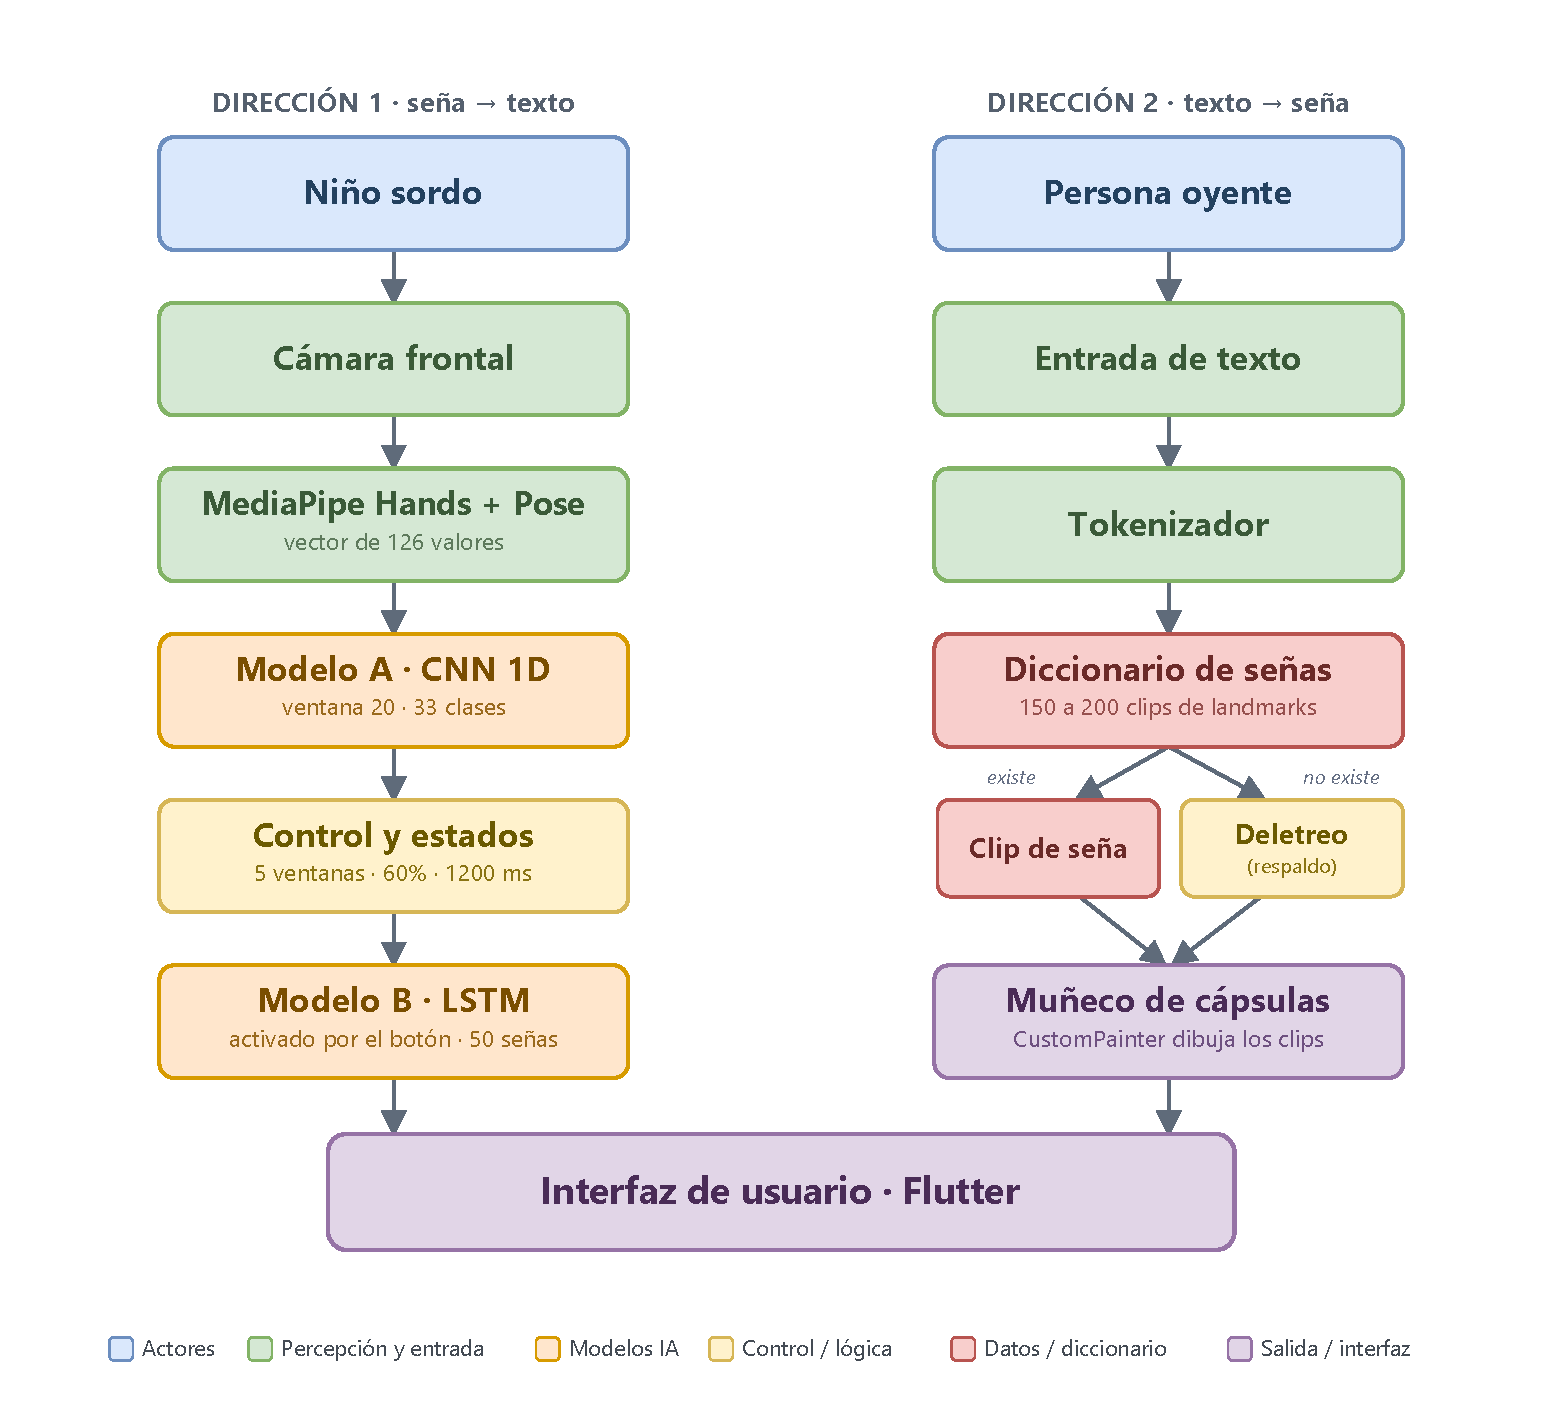
\includegraphics[width=\textwidth]{Figures/Implementacion/arquitectura.pdf}
\caption[Arquitectura general del sistema de comunicación LESHO]{Arquitectura general del sistema de comunicación \acrshort{lesho}. Se muestran los dos pipelines de comunicación y su convergencia en la interfaz de usuario compartida. Todo el procesamiento ocurre en el dispositivo, sin conexión a internet. Fuente: Elaboración propia.}
\label{fig:figure-arquitectura-lesho}
\end{figure}

La \autoref{fig:figure-arquitectura-lesho} deja ver que ambos pipelines comparten el
dispositivo y convergen en una interfaz común, pero recorren rutas independientes. En la
Dirección 1, el flujo desciende desde la cámara frontal hasta el Modelo B: cada capa entrega
su resultado a la siguiente, y el módulo de control acumula en el deletreo las letras que
el Modelo A confirma, o bien abre la ventana de grabación de una seña dinámica cuando la
persona usuaria acciona el control de grabación. En la Dirección 2, el texto escrito se descompone en la
secuencia de señas correspondiente y se entrega al muñeco de cápsulas, que la reproduce de
forma visual; cuando una palabra no existe en el diccionario, el sistema recurre al deletreo
letra por letra. Esta separación en dos rutas permite optimizar cada dirección por separado:
la primera prioriza la latencia del reconocimiento en tiempo real, mientras que la segunda
prioriza la claridad de la representación. El hecho de que ambas rutas se ejecuten por
completo en el dispositivo, sin depender de un servidor externo, es lo que garantiza el
funcionamiento sin conexión a internet y protege la privacidad de las imágenes capturadas por
la cámara, que nunca abandonan el teléfono.

\subsection{Vista Funcional del Sistema}

Más allá de su estructura interna, el sistema puede entenderse desde la experiencia de sus
dos usuarios. La \autoref{fig:figure-funcional} resume el recorrido funcional de cada
dirección de comunicación, con los pasos que percibe el usuario desde la acción inicial hasta
el resultado visible.

\begin{figure}[H]
\centering
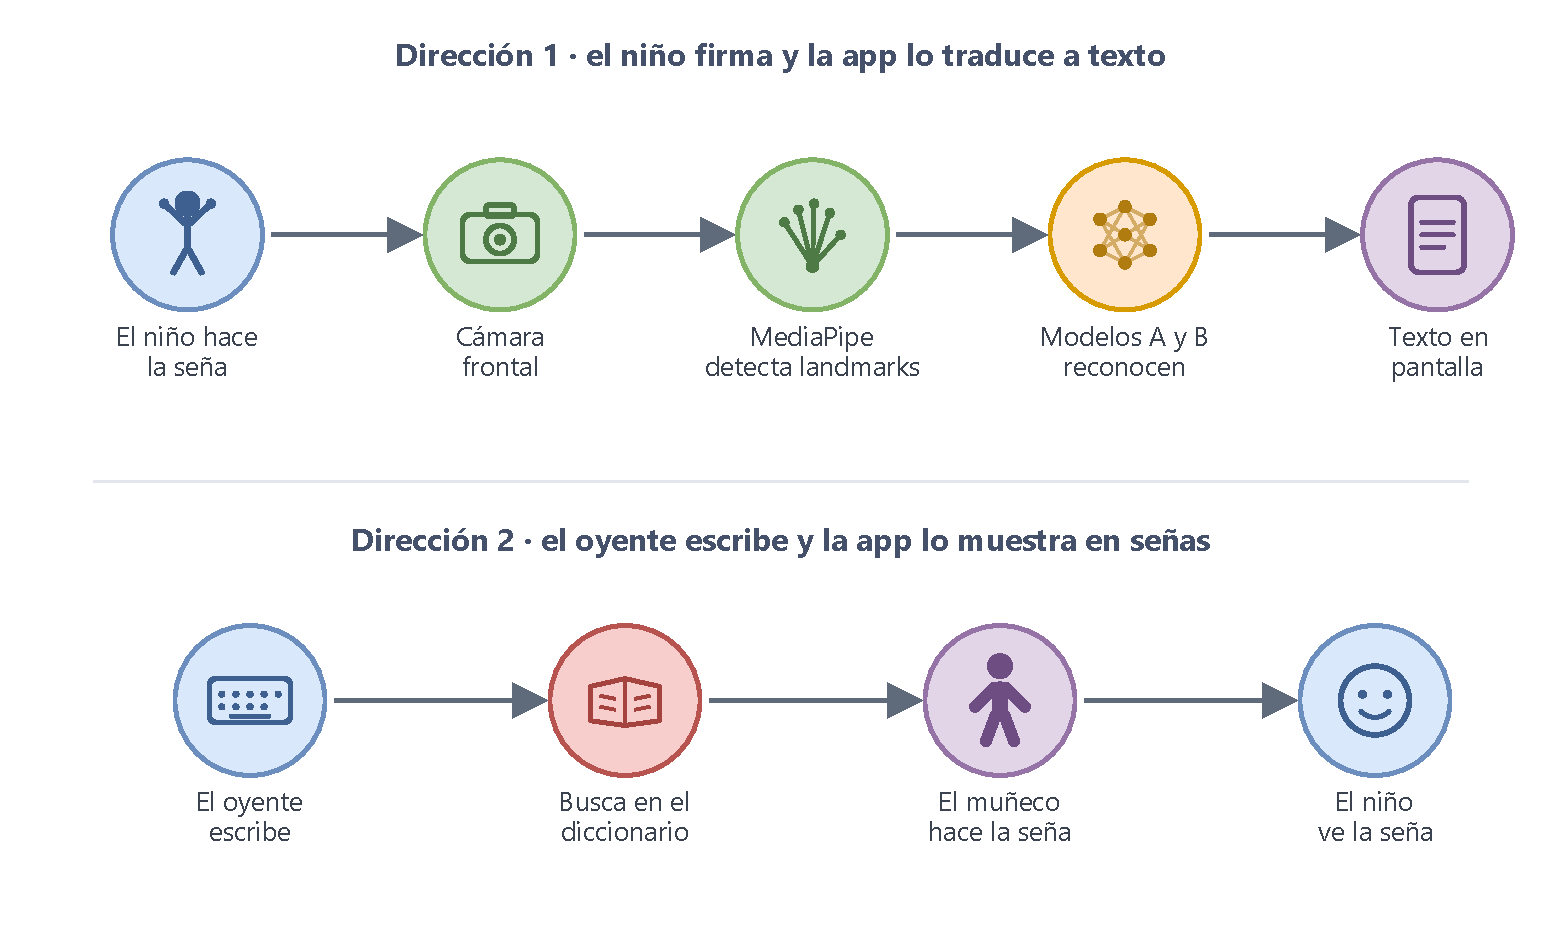
\includegraphics[width=\textwidth]{Figures/Implementacion/funcional.pdf}
\caption[Vista funcional del sistema LESHO]{Vista funcional del sistema. Se representan las dos direcciones de comunicación como flujos de operación: en la Dirección 1 el niño ejecuta la seña, la cámara la capta, MediaPipe extrae los landmarks, los modelos A y B la reconocen y el resultado aparece como texto; en la Dirección 2 la persona oyente escribe, la aplicación consulta el diccionario, el muñeco de cápsulas ejecuta la seña y el niño la observa. Fuente: Elaboración propia.}
\label{fig:figure-funcional}
\end{figure}

En la Dirección 1, el niño sordo inicia la comunicación: firma frente a la cámara y el sistema
traduce sus gestos a texto. El deletreo transcurre sin que deba tocar la pantalla, mientras
que para una seña completa delimita la grabación con el control correspondiente. En la Dirección 2, es la persona
oyente quien inicia el intercambio al escribir un mensaje que la aplicación convierte en señas
visibles para el niño. Ambos flujos comparten el mismo dispositivo y la misma interfaz, de modo
que la conversación puede alternar entre una dirección y la otra de forma natural. Esta lectura
funcional complementa la vista estructural de la arquitectura: mientras aquella muestra qué
componentes existen, esta muestra cómo se encadenan durante el uso real.

\subsection{Flujo de Reconocimiento de Señas}

El pipeline de reconocimiento de señas opera en tiempo real sobre el flujo continuo
de fotogramas capturados por la cámara frontal. Cada fotograma transita por un conjunto
de etapas que se ejecutan dentro del mismo ciclo de procesamiento antes de producir una
salida visible en pantalla.

En la primera etapa, MediaPipe Hands analiza el fotograma y extrae las coordenadas
tridimensionales de los 21 landmarks de cada mano detectada. Las coordenadas se
normalizan en dos pasos, restando la posición de la muñeca y dividiendo luego por el
tamaño de la mano, lo que produce un vector de 126 valores independiente de la posición
absoluta de las manos en la imagen y de su distancia a la cámara. Si no se detecta
ninguna mano con confianza suficiente, el fotograma se descarta.

Los vectores normalizados se acumulan en una ventana rodante de los últimos 20
fotogramas, que se entrega al Modelo A. El modelo devuelve una distribución de
probabilidad sobre las 33 clases. El módulo de control aplica entonces el
filtro de persistencia temporal: la misma clase debe aparecer como predicción
dominante durante al menos 5 ventanas consecutivas con una confianza igual o
superior al 60\,\% para que se confirme una detección. Una vez confirmada, se activa un
período de enfriamiento de 1200 milisegundos durante el cual no se aceptan nuevas
detecciones. El resultado de la detección determina el siguiente paso: si la clase
corresponde a una letra, se añade al buffer de texto visible en pantalla, y si es REPOSO
no se produce ninguna acción.

El reconocimiento de señas dinámicas sigue una ruta distinta, que la persona usuaria
delimita de forma explícita. Al pulsar el botón de grabación, el módulo de control activa
el modo dinámico y comienza a acumular la secuencia de vectores de landmarks; al pulsarlo
de nuevo para detener, envía la secuencia acumulada al Modelo B, que devuelve la seña
reconocida entre las 50 clases de su vocabulario.

La \autoref{fig:figure-secuencia-senas} muestra la interacción entre los componentes
del sistema durante el reconocimiento, incluyendo la bifurcación de comportamiento
según la clase detectada por el Modelo A.

\begin{figure}[H]
\centering
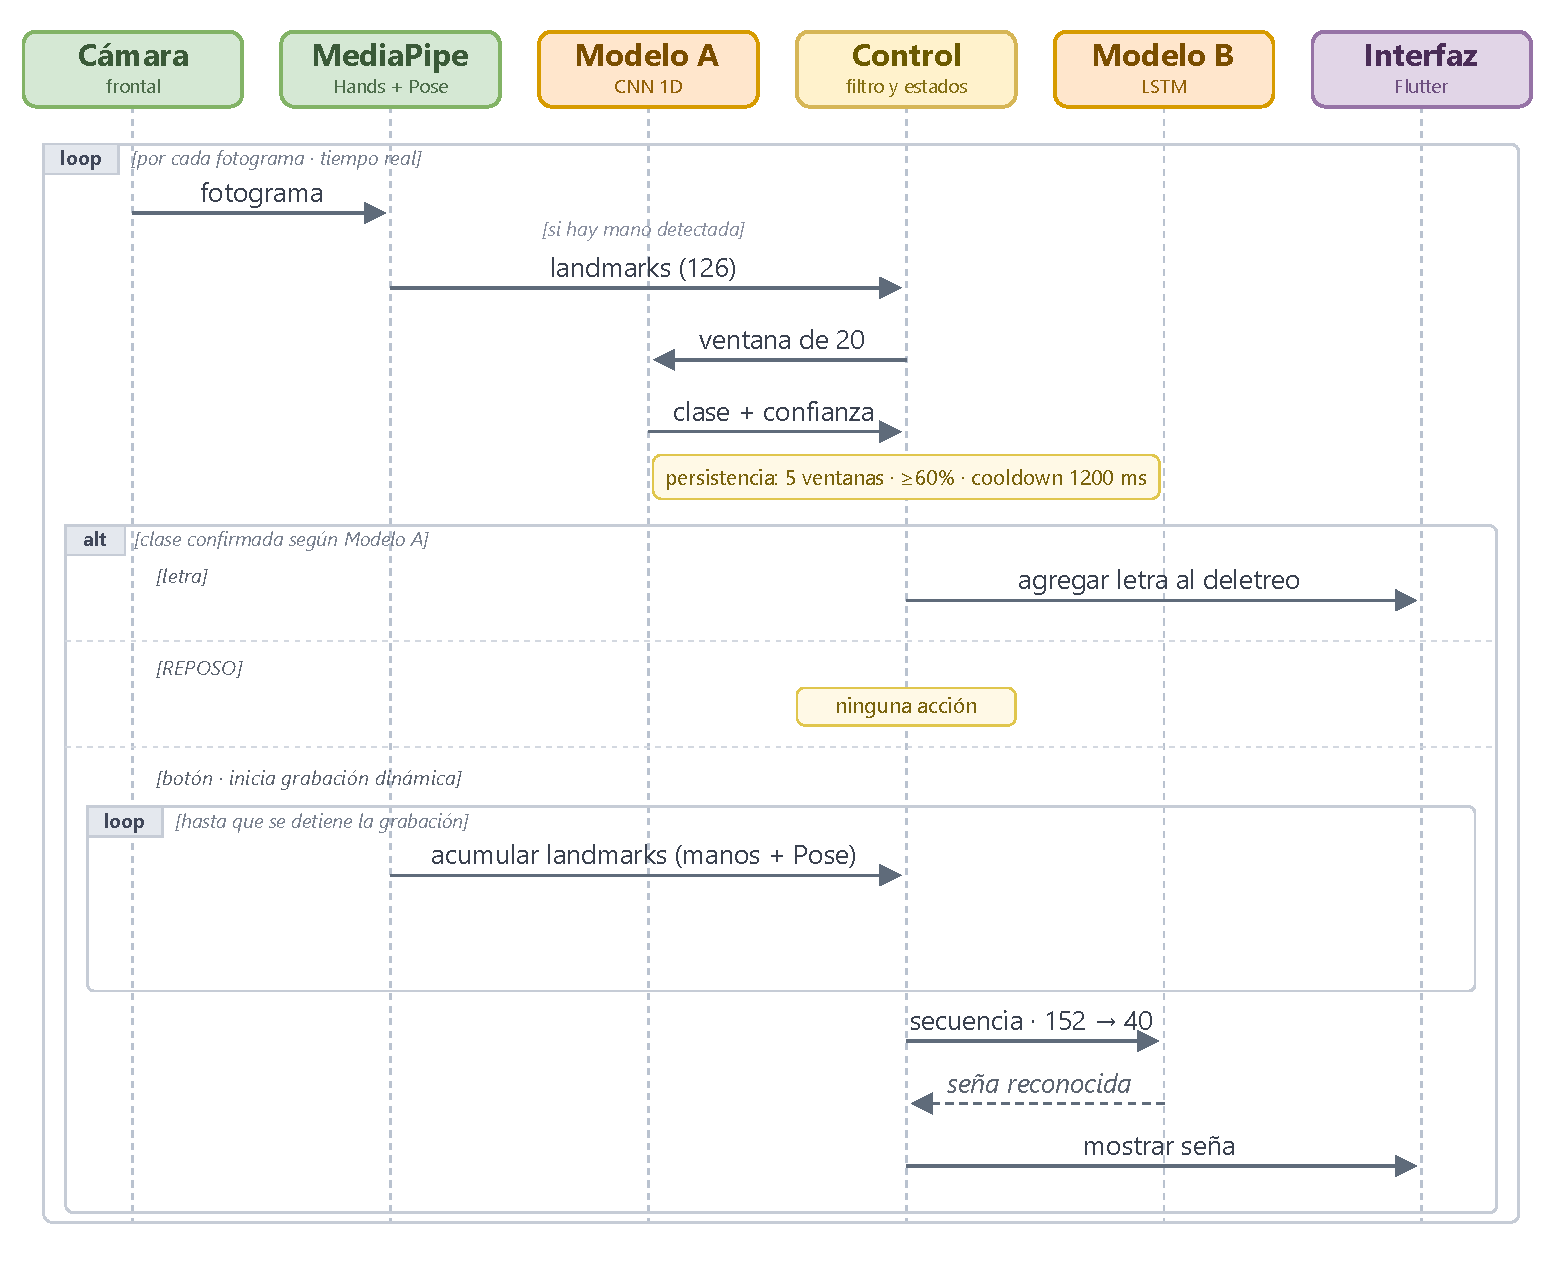
\includegraphics[width=\textwidth]{Figures/Implementacion/secuencia.pdf}
\caption[Flujo de reconocimiento de señas del sistema LESHO]{Flujo de reconocimiento de señas. El diagrama de secuencia muestra cómo el módulo de control orquesta el reconocimiento en tiempo real: recibe los landmarks de MediaPipe, arma la ventana que clasifica el Modelo A y, según la clase confirmada, agrega una letra al deletreo, no ejecuta ninguna acción ante un reposo, o abre el ciclo de grabación dinámica que acumula fotogramas hasta que la persona usuaria detiene la grabación, momento en el que el Modelo B produce la seña reconocida. Fuente: Elaboración propia.}
\label{fig:figure-secuencia-senas}
\end{figure}

En el diagrama se aprecia que el módulo de control es el eje del reconocimiento: recibe
los landmarks de MediaPipe, mantiene la ventana rodante que entrega al Modelo A y, con la
respuesta de este, aplica el filtro de persistencia antes de actuar. La rama de la
grabación dinámica es la más compleja, porque abre un ciclo en el que cada fotograma se
acumula para el Modelo B hasta que la persona usuaria cierra la grabación; solo entonces
se ejecuta la inferencia de la seña dinámica. Este diseño evita que el Modelo B, más
costoso, se ejecute de forma continua, y reserva su uso para el momento exacto en que hay
una seña completa que interpretar.

\subsection{Flujo de Texto a Seña}

El pipeline de texto a seña permite que la persona oyente comunique mensajes en
español al niño sordo utilizando el propio \acrshort{lesho}. El proceso se inicia cuando el
oyente escribe texto en el campo de entrada de la aplicación y confirma el envío.

La aplicación tokeniza el texto en palabras individuales y procesa cada una de forma
secuencial. Para cada palabra, consulta el diccionario de señas. Si existe un clip
correspondiente a esa palabra, se encola para reproducción. Si la palabra no está
registrada en el diccionario, el sistema activa el mecanismo de respaldo: la palabra se
descompone en letras y cada letra se busca individualmente en el diccionario, que
siempre contiene las 30 letras del alfabeto dactilológico del \acrshort{lesho}. Los clips
resultantes se reproducen en secuencia sobre el muñeco en la pantalla del dispositivo,
orientada hacia el niño sordo.

La \autoref{fig:figure-secuencia-texto} muestra el flujo completo del pipeline de
texto a seña, incluyendo la bifurcación entre el camino principal y el mecanismo de
respaldo por deletreo.

\begin{figure}[H]
\centering
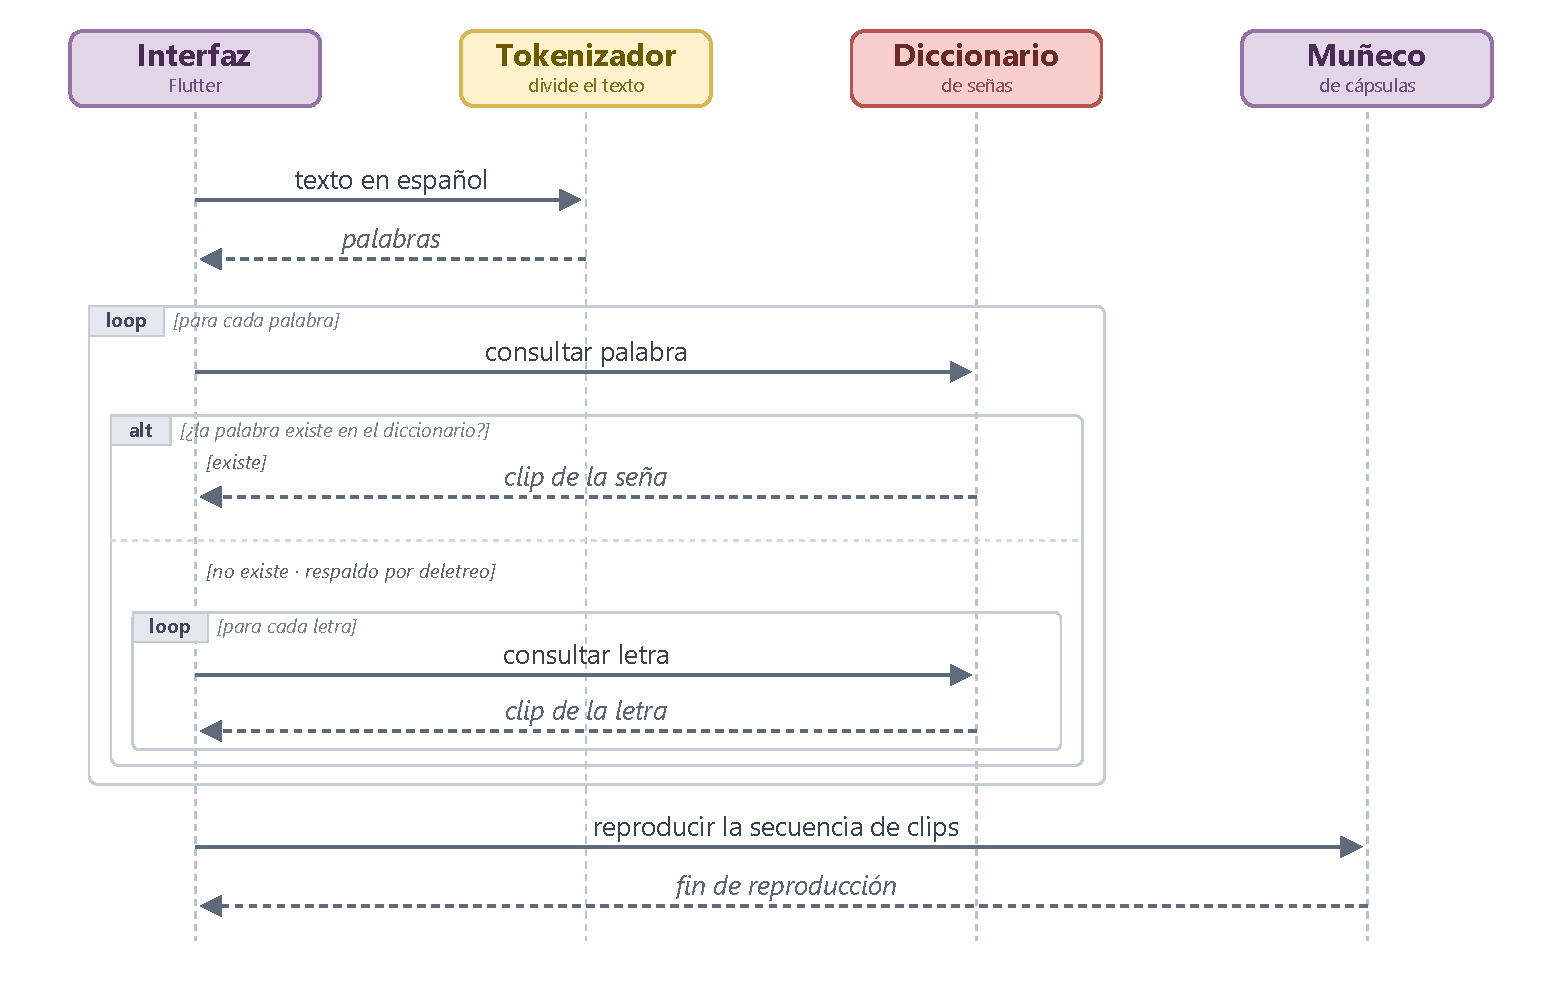
\includegraphics[width=\textwidth]{Figures/Implementacion/texto_sena.pdf}
\caption[Flujo del pipeline de texto a seña del sistema LESHO]{Flujo de texto a seña. El diagrama de secuencia muestra cómo la interfaz tokeniza el texto que escribe la persona oyente y, por cada palabra, consulta el diccionario de señas: si la palabra existe recupera el clip de su seña, y si no existe recurre al respaldo de deletreo, recuperando el clip de cada letra. Una vez reunida la secuencia, el muñeco de cápsulas la reproduce en pantalla. Fuente: Elaboración propia.}
\label{fig:figure-secuencia-texto}
\end{figure}

% ===========================================================================
\section{Implementación de la Aplicación Móvil}
\label{sec:implementacion-app}
% ===========================================================================

La aplicación se desarrolla con \textit{Flutter} como \textit{framework} multiplataforma,
utilizando \textit{Dart} como lenguaje de programación. Esta elección permite compilar
una única base de código para \textit{Android}, iOS y la web desde el mismo repositorio.
El objetivo principal de la implementación es \textit{Android}, dado que es la
plataforma predominante en el contexto hondureño. La distribución no requiere publicación
en tiendas de aplicaciones oficiales: la aplicación se empaqueta como un archivo
\acrfull{apk} instalable directamente en el dispositivo.

% ---------------------------------------------------------------------------
\subsection{Estructura del Proyecto}
\label{sec:estructura-proyecto}
% ---------------------------------------------------------------------------

El repositorio se organiza en dos partes diferenciadas. La parte de la aplicación
móvil contiene el código \textit{Flutter}, los modelos exportados a formato
\acrshort{tflite} empaquetados como \textit{assets}, los archivos de etiquetas y los
clips de landmarks del diccionario de señas. La parte del \textit{pipeline} de
entrenamiento contiene los \textit{scripts} de captura, preprocesamiento y entrenamiento
en \textit{Python}, junto con el conjunto de datos en formato \textit{CSV}.

Los paquetes principales de los que depende la aplicación son: el paquete
\texttt{camera}, para la captura del flujo de video en tiempo real desde la cámara
frontal; y el paquete \texttt{tflite\_flutter}, para la ejecución de inferencia con los
modelos clasificadores dentro del proceso de \textit{Dart}. La representación visual de
las señas en el módulo de texto a seña no utiliza un reproductor de video externo, sino
un muñeco animado que se dibuja directamente con el \textit{CustomPainter} de
\textit{Flutter} a partir de los clips de landmarks. Todos los \textit{assets} críticos
(modelos y clips) se incluyen dentro del paquete de la aplicación, lo que garantiza el
funcionamiento sin conexión a internet.

% ---------------------------------------------------------------------------
\subsection{Captura y Extracción de Características}
\label{sec:captura-landmarks}
% ---------------------------------------------------------------------------

La aplicación activa la cámara frontal del dispositivo mediante el paquete
\texttt{camera} y procesa el flujo de video a aproximadamente 30 fotogramas por
segundo. Cada fotograma se entrega a \textit{MediaPipe Hands}, que devuelve las
coordenadas tridimensionales de los 21 \textit{landmarks} de la mano detectada.
La integración de \textit{MediaPipe} con \textit{Flutter} se realiza mediante un
canal de plataforma (\textit{platform channel}) que ejecuta \textit{MediaPipe} en un
hilo nativo en segundo plano, de modo que el hilo de la interfaz permanece libre y la
captura no se bloquea.

Cada mano detectada aporta 21 \textit{landmarks} con 3 coordenadas ($x$, $y$, $z$), de
modo que las dos manos conforman un vector de 126 valores. Antes de entregarlos a los
modelos, los valores se normalizan en dos pasos. Primero se restan las coordenadas del
\textit{landmark} 0, correspondiente a la muñeca, de cada mano, con lo que el vector
resultante deja de depender de la posición absoluta de las manos dentro del cuadro de la
cámara. Después se divide por el tamaño de la mano, con lo que tampoco depende de la
distancia a la que se encuentre el usuario. Ambas operaciones incrementan la robustez del
clasificador ante distintas posiciones del dispositivo y del usuario. En la ruta de señas dinámicas se ejecuta además
\textit{MediaPipe Pose}, que aporta la ubicación de las manos respecto al cuerpo. Si
\textit{MediaPipe Hands} no detecta ninguna mano con confianza suficiente en un
fotograma dado, ese fotograma se descarta y no se entrega a ninguno de los modelos.

% ---------------------------------------------------------------------------
\subsection{Módulo de Reconocimiento de Señas}
\label{sec:modulo-reconocimiento}
% ---------------------------------------------------------------------------

El módulo de reconocimiento de señas implementa el \textit{pipeline} de la
Dirección 1 del sistema y opera de forma continua sobre el flujo de fotogramas
procesados por \textit{MediaPipe}.

\subsubsection{Inferencia con el Modelo A}

Los vectores normalizados de 126 valores se acumulan en una ventana rodante de 20
fotogramas que se entrega al Modelo A, implementado como una red convolucional 1D
(\acrshort{cnn} 1D) y ejecutado mediante \acrshort{tflite}. El modelo devuelve una
distribución de probabilidad sobre las 33 clases con que fue entrenado: las 30 letras del
alfabeto dactilológico del \acrshort{lesho}, la clase de reposo y las dos señas de control
que se evaluaron durante el desarrollo y que la versión final no utiliza. La clase
con mayor probabilidad constituye la predicción de la ventana actual. Clasificar una
ventana y no un fotograma aislado es lo que permite reconocer las cinco letras que se
ejecutan con movimiento: la J, la Ñ, la Z, la LL y la RR.

\subsubsection{Filtro de Persistencia Temporal y Período de Enfriamiento}

El módulo de control no actúa sobre ninguna predicción individual. Mantiene un
contador de ventanas consecutivas en las que la misma clase aparece como predicción
dominante. Solo cuando esa clase acumula cinco ventanas consecutivas con una confianza
igual o superior al 60\,\% se confirma la detección. Tras la confirmación, se activa
un período de enfriamiento de 1200 milisegundos durante el cual el módulo ignora nuevas
predicciones. Este mecanismo evita detecciones repetidas causadas por la transición
lenta de la mano entre una seña y la siguiente.

\subsubsection{Máquina de Estados del Reconocimiento}

El módulo de control opera con dos estados diferenciados. En el estado de deletreo, el
sistema clasifica de forma continua la ventana rodante de fotogramas y actúa según la
clase confirmada: si es una letra, la añade al \textit{buffer} de texto visible en
pantalla, y si es REPOSO no produce ninguna acción. El módulo transita al estado de
grabación dinámica cuando la persona usuaria pulsa el control de grabación. En ese estado
el sistema acumula los vectores de \textit{landmarks} de fotogramas sucesivos en lugar de
clasificarlos por ventana. Al detener la grabación, el módulo entrega la secuencia
acumulada al Modelo B y regresa al estado de deletreo.

\subsubsection{Inferencia con el Modelo B}

El Modelo B, implementado como una red \acrshort{lstm} y ejecutado mediante
\acrshort{tflite}, recibe la secuencia acumulada durante la grabación. Cada
fotograma de la secuencia combina la configuración de las manos con la ubicación de
estas respecto al cuerpo, obtenida con \textit{MediaPipe Pose}, para conformar una
entrada de 152 valores; la secuencia se remuestrea a una longitud fija de 40 fotogramas
antes de la inferencia. El modelo devuelve una distribución de probabilidad sobre las
50 clases dinámicas del vocabulario reconocido. La seña con mayor probabilidad se
muestra en la interfaz como resultado del reconocimiento, y el sistema regresa al
estado de deletreo para continuar el ciclo.

% ---------------------------------------------------------------------------
\subsection{Módulo de Texto a Seña}
\label{sec:modulo-texto-sena}
% ---------------------------------------------------------------------------

El módulo de texto a seña implementa el \textit{pipeline} de la Dirección 2 del
sistema. La persona oyente ingresa un mensaje en español mediante un campo de texto
de la interfaz. El módulo divide el texto en palabras individuales mediante un
tokenizador que separa por espacios y descarta puntuación.

Para cada palabra resultante, el módulo consulta el diccionario de señas. Si la palabra
tiene un clip correspondiente en el diccionario, ese clip se añade a la cola de
reproducción. Si la palabra no se encuentra en el diccionario, el módulo la descompone
letra por letra y añade a la cola el clip de cada letra del alfabeto dactilológico,
aplicando así el mecanismo de respaldo por deletreo descrito en el diseño del sistema.
Una vez procesadas todas las palabras, el muñeco reproduce la cola de clips de forma
secuencial, mostrando cada seña de forma ordenada en pantalla.

El diccionario de señas tiene como objetivo entre 150 y 200 entradas, que incluyen
las 30 letras del alfabeto dactilológico, las 50 señas dinámicas del vocabulario del
Modelo B, y señas adicionales de vocabulario común agrupadas por categorías: números,
colores, vínculos familiares, emociones, entorno escolar y necesidades básicas.

% ---------------------------------------------------------------------------
\subsection{Interfaz de Usuario}
\label{sec:interfaz-usuario}
% ---------------------------------------------------------------------------

La interfaz de usuario se diseña considerando que el usuario principal es un niño
sordo. Los elementos interactivos tienen un tamaño generoso para facilitar la
interacción táctil, y la retroalimentación visual de cada acción es clara e
inmediata. La aplicación presenta dos pantallas principales: la pantalla de
reconocimiento, que muestra la vista de la cámara frontal y el texto acumulado del
deletreo o la seña dinámica reconocida, y la pantalla de texto a seña, donde la
persona oyente escribe el mensaje y la aplicación reproduce la secuencia de señas
correspondiente.

La transición entre pantallas es explícita y controlada por el usuario, de modo que
en cada momento solo uno de los dos \textit{pipelines} permanece activo. La
aplicación no requiere conexión a internet en ninguna de sus funciones, dado que los
modelos de clasificación y el diccionario de señas están empaquetados dentro del
\acrshort{apk}.

% ===========================================================================
\section{Pruebas y Resultados Preliminares}
% ===========================================================================

A lo largo de las semanas de desarrollo, el sistema no se armó de una sola vez, sino que se
fue construyendo y probando por partes. Esta sección recoge esas pruebas y los resultados
preliminares que arrojaron. Conviene aclararlo desde el inicio: son resultados obtenidos con
pocos datos, cuyo propósito fue orientar las decisiones de diseño y confirmar que cada pieza
funcionaba antes de invertir en la grabación del conjunto de datos definitivo. La evaluación
formal, con los cuatro participantes, se desarrolla en el capítulo de resultados.

El enfoque fue iterativo: cada componente se probó apenas estuvo integrado, con un conjunto
reducido de muestras y directamente sobre un teléfono real de gama baja, un Samsung Galaxy
A13. Así se pudo confirmar de forma temprana que la tubería completa funcionaba en el
dispositivo y detectar los problemas propios de la ejecución \textit{on-device} desde el
inicio, antes de escalar el conjunto de datos.

Durante estas semanas se llevaron al dispositivo los tres bloques del sistema. El deletreo del
alfabeto (Modelo A) se probó primero, pues utiliza una sola mano y no requiere MediaPipe Pose,
y funcionó de forma fluida en el teléfono. Enseguida se integró la tubería completa del Modelo
B, con MediaPipe Pose, el marco de referencia del cuerpo y el preprocesamiento de la secuencia;
esta tubería se validó comparando su salida en el teléfono contra la implementación de
referencia en \textit{Python}, para asegurar que ambas produjeran los mismos vectores. Para
probar el reconocimiento de señas dinámicas se entrenó un modelo reducido con diez palabras y
una sola persona, concebido como prueba de concepto de la tubería y no como un modelo
generalizable. Por último, la Dirección 2 se probó reproduciendo señas en el muñeco de cápsulas
sobre el mismo dispositivo.

Las pruebas con este conjunto reducido de datos evidenciaron lo siguiente:

\begin{itemize}
    \item El deletreo del alfabeto funciona de forma estable en el teléfono, con una respuesta
    suficientemente ágil para escribir letra por letra.
    \item El Modelo B aprende la tarea con los datos de una sola persona, alcanzando una
    exactitud de validación cercana al 99\,\%. Este valor confirma que la arquitectura y el
    preprocesamiento son correctos, pero es optimista: al provenir de una única persona, no
    anticipa el desempeño con personas nuevas.
    \item Las señas que se distinguen por el lugar de articulación se reconocen con solidez.
    Por ejemplo, HOSPITAL, que se ejecuta en una zona bien diferenciada, se identifica sin
    problema. En cambio, las señas que comparten lugar y difieren solo en la forma o el
    movimiento de la mano, como HOLA y AGUA, se confunden con facilidad y son las que más se
    benefician de contar con más datos y más personas.
\end{itemize}

Más allá de las cifras, estas pruebas dejaron aprendizajes que moldearon el diseño final. El
primero fue la importancia de incorporar la punta del índice a la ubicación de la mano en el
cuerpo: muchas señas se hacen apuntando con los dedos a una zona, como HOLA hacia la frente o
AGUA hacia la boca, mientras la muñeca permanece a un costado; sin la punta del índice, ambas
señas colapsaban en una sola. El segundo fue la corrección del factor de aspecto: el conjunto
de datos se grabó en formato 16:9 y el teléfono entrega 3:4, de modo que las coordenadas debían
corregirse en vivo según el aspecto real de la cámara, pues de lo contrario el modelo confundía
casi todas las señas. El tercero fue una limitación del hardware: el Samsung Galaxy A13 entrega
alrededor de cinco fotogramas por segundo cuando procesa dos manos junto con MediaPipe Pose, una
tasa baja que obliga a capturar la seña con cuidado y a sostener la posición inicial. El
deletreo, al usar una sola mano y no ejecutar Pose, no se ve afectado por esta limitación.

En conjunto, estos resultados preliminares validan la viabilidad técnica del sistema: la
tubería completa, desde la cámara hasta la clasificación y la representación en el muñeco,
funciona por entero en el dispositivo y sin conexión a internet. También delimitan con claridad
el trabajo que resta, que es ampliar el conjunto de datos a varias personas para que el
reconocimiento de señas dinámicas generalice más allá de las condiciones de grabación. Ese
conjunto de datos completo y su evaluación formal se presentan en el capítulo siguiente.


%%% Part 5: Análisis de Resultados %%%
\cleardoublepage
\thispagestyle{empty} % Sin encabezado, sin pie de página

% === Registrar la parte en el índice ===
\refstepcounter{part} % Incrementa el contador de partes
\addcontentsline{toc}{part}{Parte \thepart:Resultados y Análisis }

% === Fondo decorativo ===
\AddToShipoutPictureBG*{%
	\put(0,0){%
		\parbox[b][\paperheight]{\paperwidth}{%
			\vfill
			\centering
			
\includegraphics[width=\paperwidth,height=\paperheight]{Figures/Theme/Front-Page-E.pdf}%
			\vfill
		}%
	}%
}

% === Contenido de la portada de parte ===
\vspace*{\fill}
\begin{center}
	{\Huge\bfseries Parte \thepart}\\[2cm]
	{\Huge\bfseries RESULTADOS Y ANÁLISIS}
\end{center}
\vspace*{\fill}

\clearpage

\chapter[Resultados y Análisis]{Resultados y Análisis}
\label{chap:resultados}

\insertminitoc
\parindent0pt


\section{Presentación de los resultados}

Este capítulo presenta la evaluación del sistema de reconocimiento del \Acrshort{lesho}. Se organiza en seis partes: el desempeño del modelo del alfabeto dactilológico (Modelo A), el desempeño del modelo de señas dinámicas (Modelo B), la comparación entre ambos, la evaluación del sistema ejecutándose sobre el dispositivo, los instrumentos diseñados para medir la usabilidad con las personas usuarias, y una discusión integral de los hallazgos.

La evaluación de los modelos se realizó con una división estratificada por clase y agrupada por toma: ninguna toma de captura cruzó de la partición de entrenamiento a la de prueba, y todas las clases con datos aparecen en las particiones. Esta decisión evita la fuga de datos que produce la división aleatoria por ventana, en la que fragmentos casi idénticos de una misma grabación caen a la vez en entrenamiento y prueba e inflan la exactitud de forma ficticia. En consecuencia, las cifras que se reportan miden el desempeño sobre tomas que el modelo no vio nunca. Todas las figuras de este capítulo son de elaboración propia.


\section{Desempeño del Modelo A (alfabeto dactilológico)}

El Modelo A clasifica una ventana temporal corta de fotogramas de landmarks en las 33 clases con que fue entrenado: las 30 letras del alfabeto dactilológico, la clase de reposo y las dos señas de control que se evaluaron durante el desarrollo y que la versión final del sistema no utiliza. Estas dos últimas aparecen en las figuras de este capítulo con las etiquetas INICIO y FIN, que son los nombres con que se grabaron. La Tabla~\ref{tab:metricas-a} resume sus métricas globales sobre la partición de prueba.

\begin{table}[h!]
\centering
\begin{tabular}{lc}
\hline
\textbf{Métrica} & \textbf{Valor} \\
\hline
Exactitud global & 99.54\% \\
Puntaje F1 (macro) & 0.995 \\
Número de clases & 33 \\
Muestras de prueba & 4,364 \\
Parámetros del modelo & 24,929 \\
Tamaño en \Acrshort{tflite} & 33.9 KB \\
\hline
\end{tabular}
\caption{Métricas globales del Modelo A sobre la partición de prueba.}
\label{tab:metricas-a}
\end{table}

La exactitud global de \textbf{99.54\%} y el puntaje F1 macro de \textbf{0.995} indican que el modelo separa con solidez las clases del alfabeto. El valor F1 macro, que promedia el desempeño de todas las clases por igual sin importar cuántas muestras tenga cada una, confirma que el resultado no depende de unas pocas clases mayoritarias.

La Figura~\ref{fig:curvas-a} muestra la evolución de la exactitud y de la pérdida durante el entrenamiento, tanto en el conjunto de entrenamiento como en el de validación.

\begin{figure}[htbp]
    \centering
    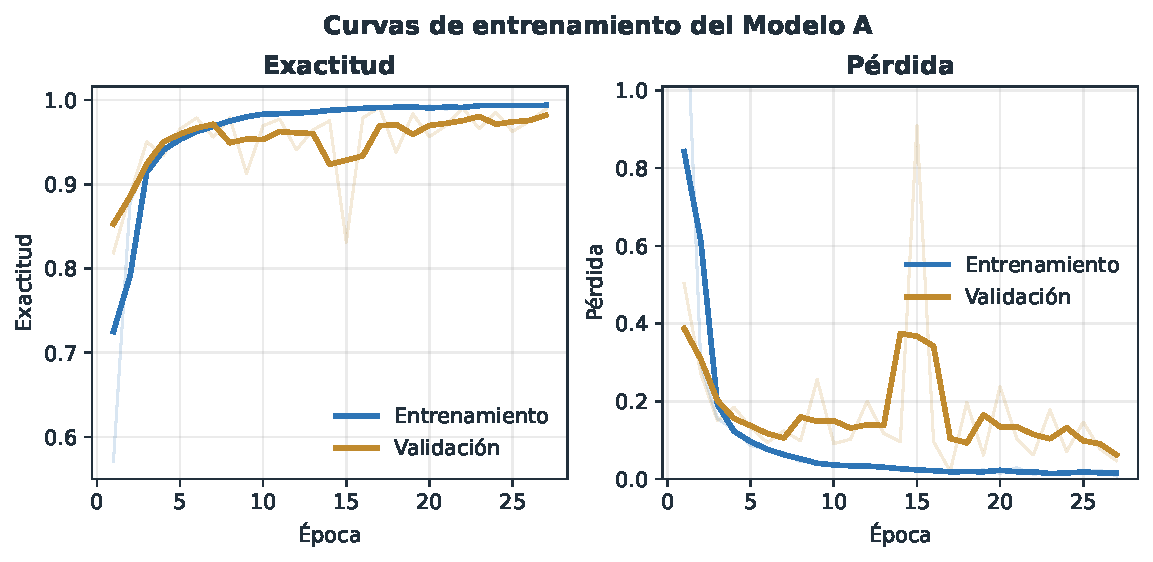
\includegraphics[width=1\linewidth]{Figures/Resultados/curvas_entrenamiento_a.pdf}
    \caption[Curvas de entrenamiento del Modelo A]{Curvas de entrenamiento del Modelo A: exactitud y pérdida por época. La línea marcada es el promedio móvil y la línea tenue el valor de cada época. Fuente: Elaboración propia.}
    \label{fig:curvas-a}
\end{figure}

Las curvas de la Figura~\ref{fig:curvas-a} muestran una convergencia estable. La pérdida de validación desciende junto con la de entrenamiento y no vuelve a subir de forma sostenida, lo que indica que el mecanismo de parada temprana detuvo el ajuste antes de que apareciera un sobreajuste marcado. La cercanía entre las curvas de entrenamiento y de validación es una señal de que el modelo generaliza dentro del corpus disponible.

Para observar el detalle por clase, la Figura~\ref{fig:confusion-a} presenta la matriz de confusión y la Figura~\ref{fig:f1-a} el puntaje F1 de cada clase.

\begin{figure}[htbp]
    \centering
    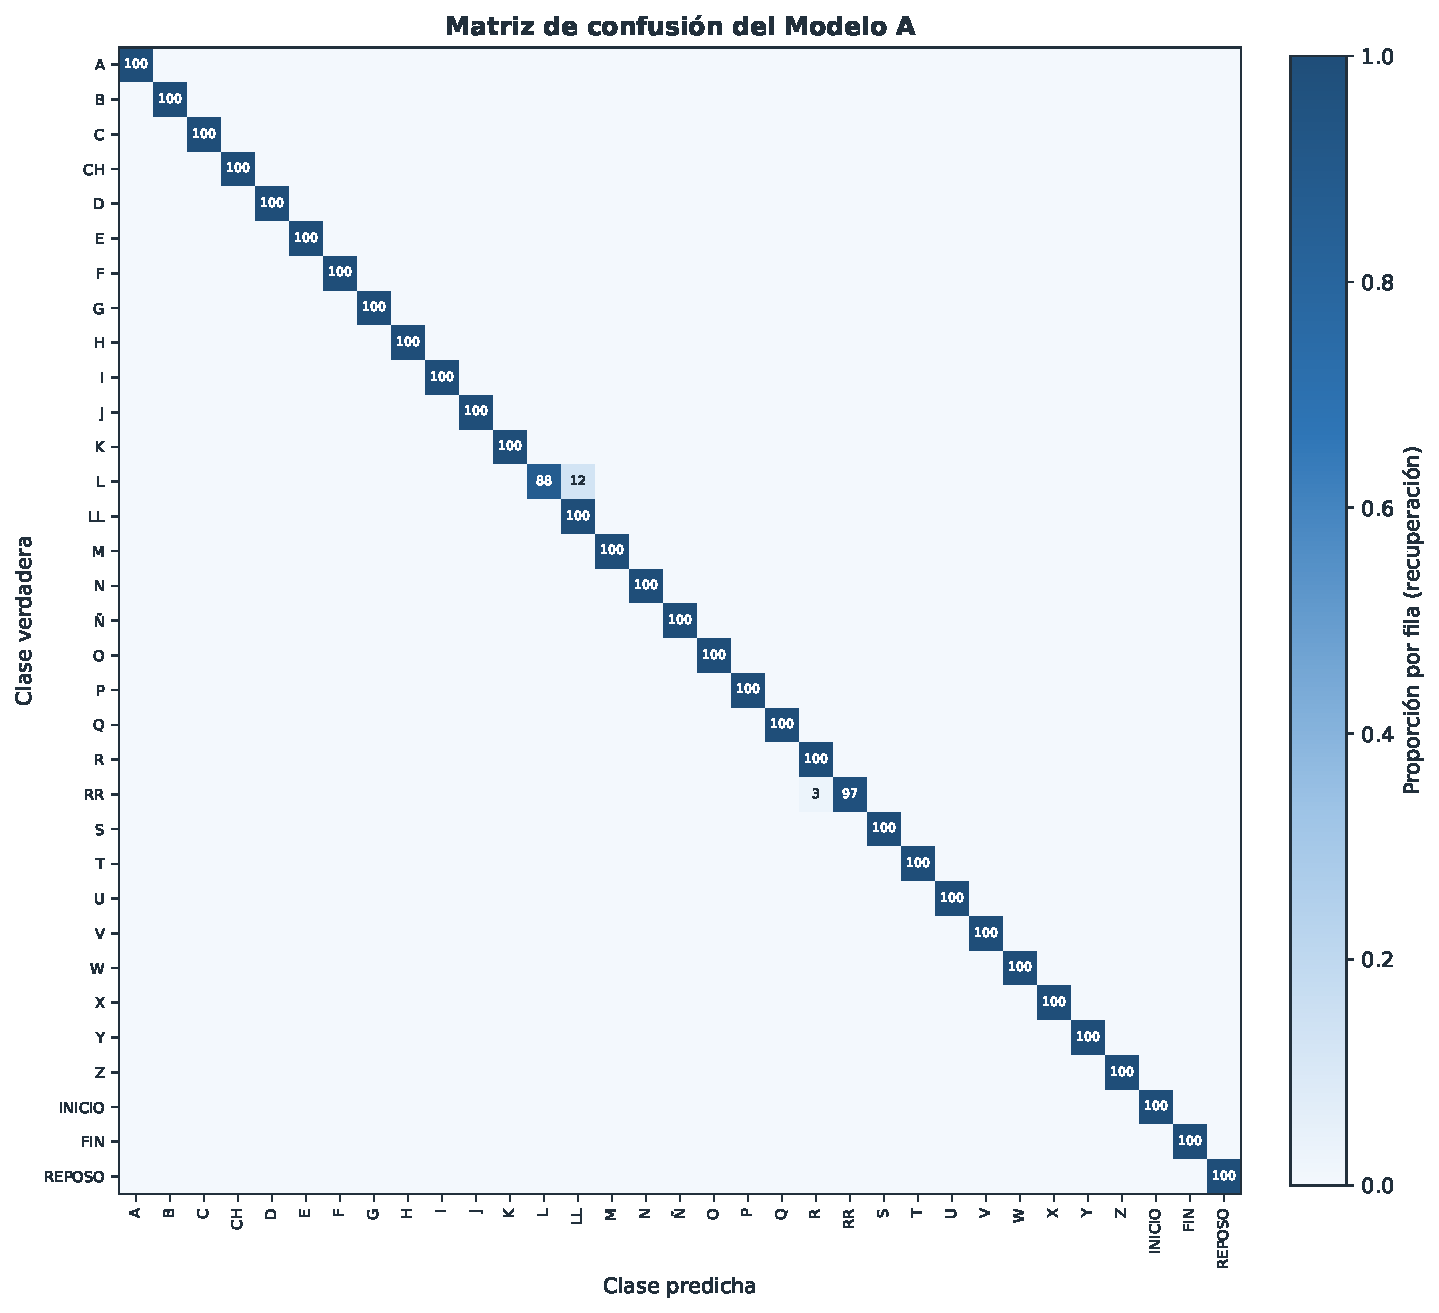
\includegraphics[width=0.9\linewidth]{Figures/Resultados/matriz_confusion_a.pdf}
    \caption[Matriz de confusión del Modelo A]{Matriz de confusión del Modelo A, normalizada por fila. Fuente: Elaboración propia.}
    \label{fig:confusion-a}
\end{figure}

En la matriz de confusión de la Figura~\ref{fig:confusion-a}, la diagonal concentra casi toda la masa, lo que refleja la alta exactitud. Las confusiones que aparecen fuera de la diagonal son coherentes con la naturaleza del alfabeto dactilológico: se dan entre letras de forma de mano parecida. Las cinco letras que se ejecutan con movimiento, que son la J, la Ñ, la Z, la LL y la RR, son las más sensibles, porque su reconocimiento depende de la trayectoria completa y esa trayectoria varía más entre personas que la forma de una pose fija.

\begin{figure}[htbp]
    \centering
    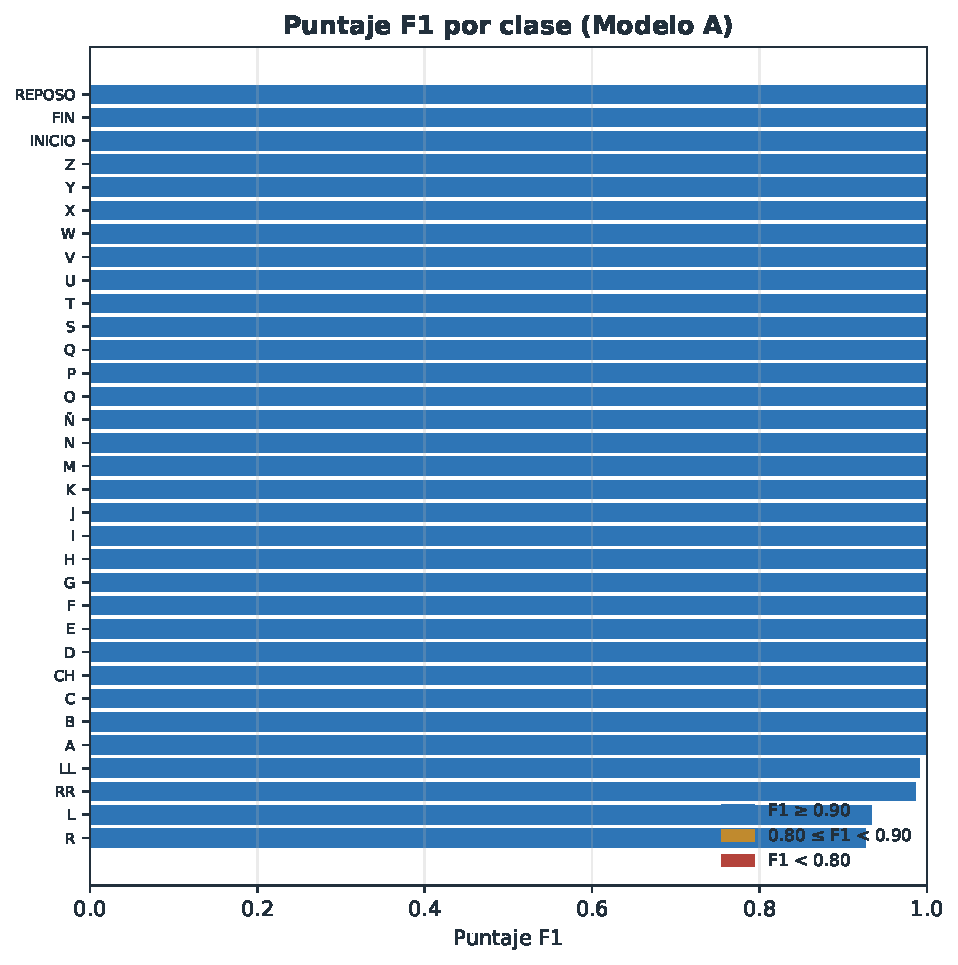
\includegraphics[width=0.68\linewidth]{Figures/Resultados/f1_por_clase_a.pdf}
    \caption[Puntaje F1 por clase del Modelo A]{Puntaje F1 por clase del Modelo A, ordenado de menor a mayor. Fuente: Elaboración propia.}
    \label{fig:f1-a}
\end{figure}

La Figura~\ref{fig:f1-a} confirma que la gran mayoría de las clases supera un F1 de 0.90. Las pocas clases con un valor menor corresponden a las letras con movimiento y a algunas letras estáticas de forma similar. Este comportamiento es el esperado y se explica por la variabilidad natural del gesto, no por un defecto del modelo.


\section{Desempeño del Modelo B (señas dinámicas)}

El Modelo B es una red \acrfull{lstm} ligera que clasifica una secuencia completa de landmarks en las 50 señas dinámicas del vocabulario. A diferencia del Modelo A, cada fotograma incorpora, además de la configuración de las manos, la ubicación de estas respecto al cuerpo, obtenida con el marco de referencia de los hombros y de las anclas de la cara. La Tabla~\ref{tab:metricas-b} resume sus métricas globales sobre la partición de prueba.

\begin{table}[h!]
\centering
\begin{tabular}{lc}
\hline
\textbf{Métrica} & \textbf{Valor} \\
\hline
Exactitud global & 98.80\% \\
Puntaje F1 (macro) & 0.988 \\
Número de señas & 50 \\
Muestras de prueba & 834 \\
Parámetros del modelo & 61,122 \\
Tamaño en \Acrshort{tflite} & 78.1 KB \\
\hline
\end{tabular}
\caption{Métricas globales del Modelo B sobre la partición de prueba.}
\label{tab:metricas-b}
\end{table}

La exactitud global de \textbf{98.80\%} y el F1 macro de \textbf{0.988} muestran que el modelo distingue con claridad las señas del vocabulario. La Figura~\ref{fig:curvas-b} presenta las curvas de entrenamiento.

\begin{figure}[htbp]
    \centering
    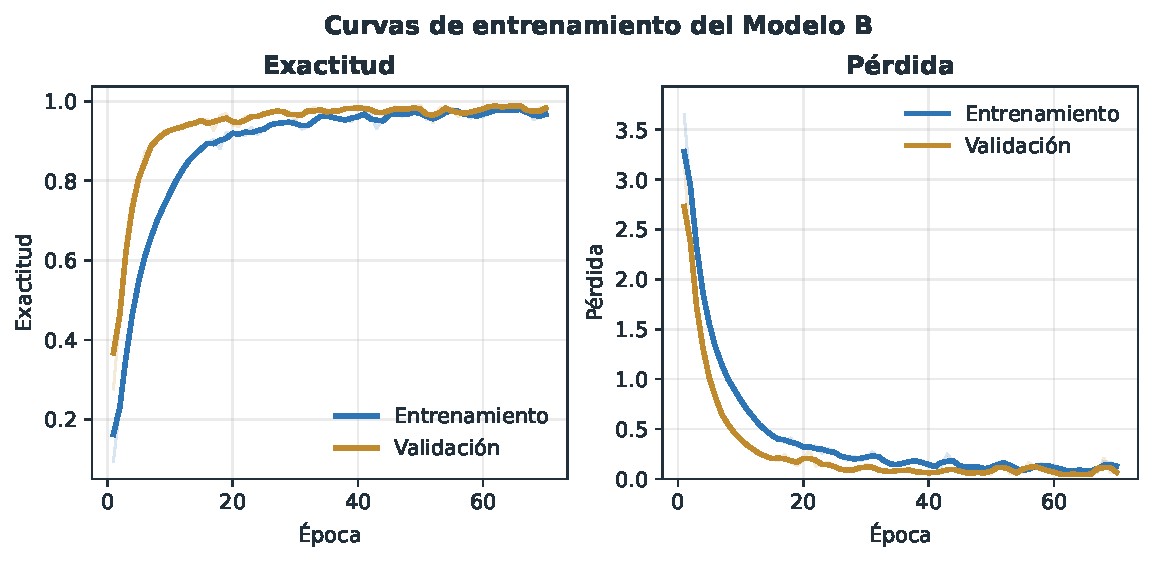
\includegraphics[width=1\linewidth]{Figures/Resultados/curvas_entrenamiento_b.pdf}
    \caption[Curvas de entrenamiento del Modelo B]{Curvas de entrenamiento del Modelo B: exactitud y pérdida por época. La línea marcada es el promedio móvil y la línea tenue el valor de cada época. Fuente: Elaboración propia.}
    \label{fig:curvas-b}
\end{figure}

Como se aprecia en la Figura~\ref{fig:curvas-b}, la validación alcanza valores altos y se mantiene cercana a la curva de entrenamiento, lo que indica que la arquitectura aprende la tarea sin un sobreajuste marcado. La parada temprana detiene el entrenamiento cuando la pérdida de validación deja de mejorar.

La Figura~\ref{fig:confusion-b} presenta la matriz de confusión de las 50 señas.

\begin{figure}[htbp]
    \centering
    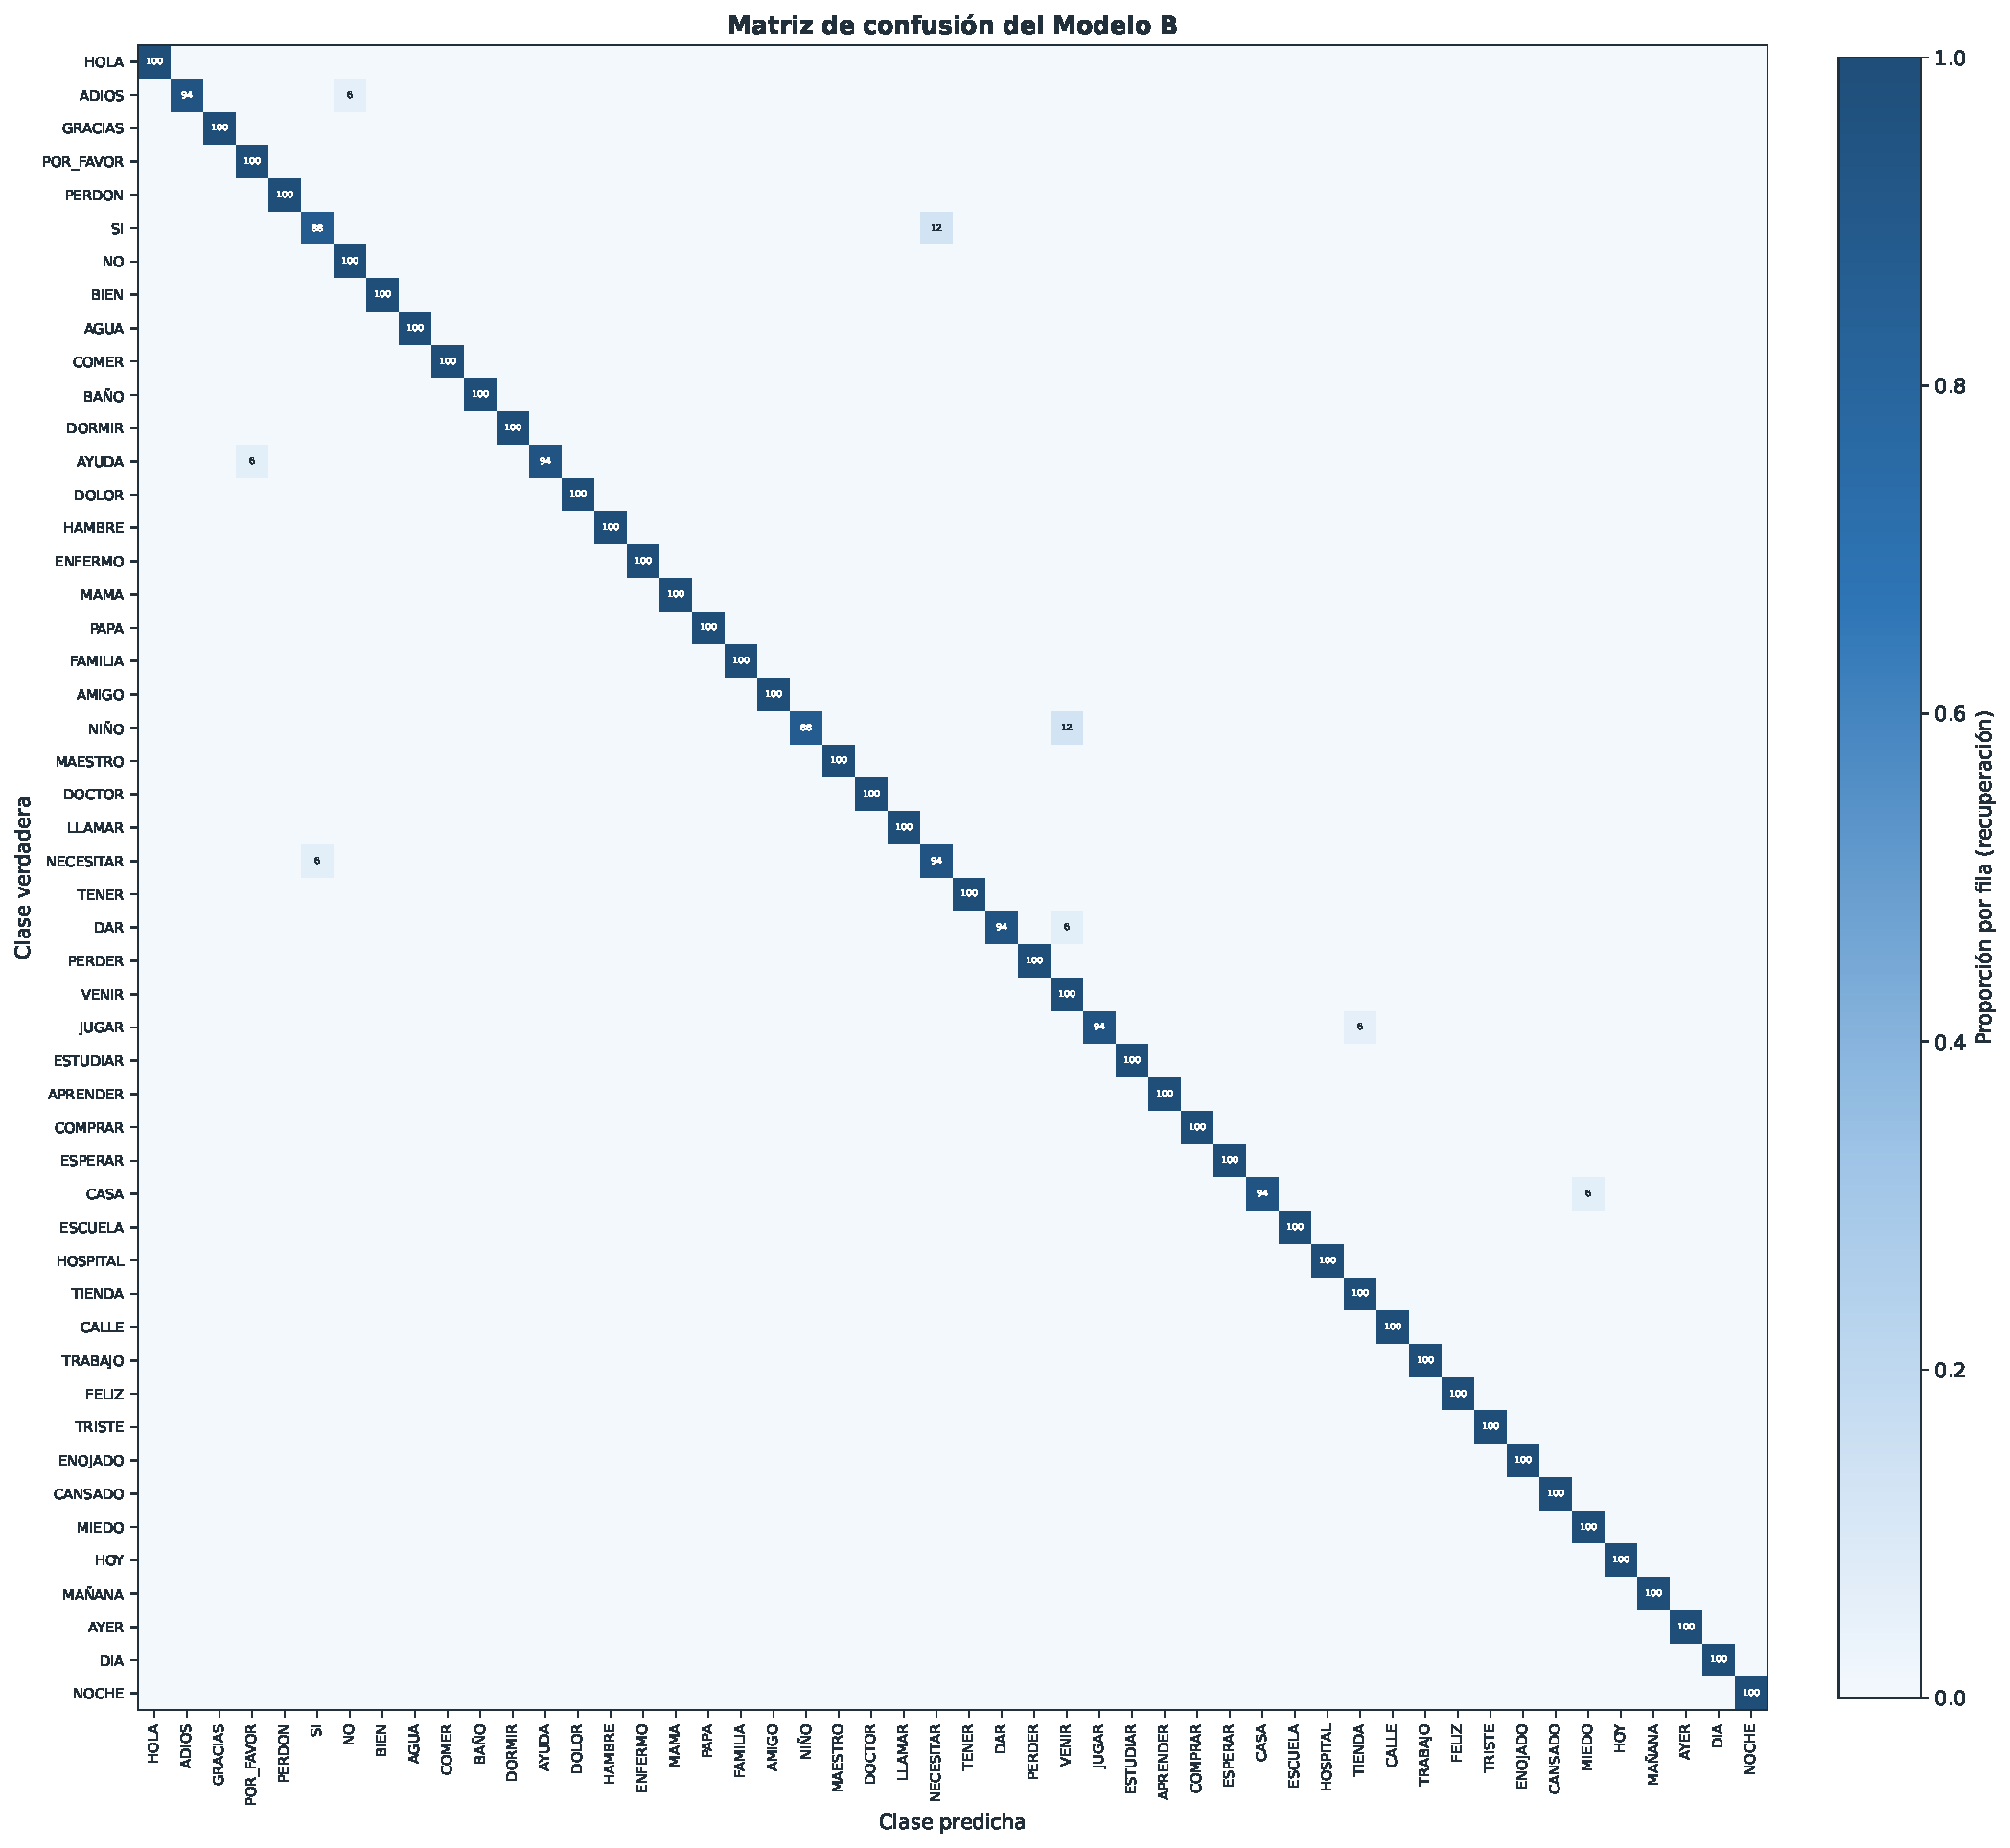
\includegraphics[width=1\linewidth]{Figures/Resultados/matriz_confusion_b.pdf}
    \caption[Matriz de confusión del Modelo B]{Matriz de confusión del Modelo B, normalizada por fila, sobre las 50 señas dinámicas. Fuente: Elaboración propia.}
    \label{fig:confusion-b}
\end{figure}

En la Figura~\ref{fig:confusion-b} la diagonal vuelve a concentrar la masa de aciertos. Las pocas confusiones que aparecen son leves y se dan entre señas que comparten el lugar de articulación y se distinguen por matices de forma o de movimiento de la mano. Este patrón valida una decisión central del diseño: incorporar la ubicación de la mano en el cuerpo, y en particular la posición de la punta del índice, fue lo que permitió separar señas que se hacen en zonas distintas de la cara, como HOLA en la frente y AGUA en la boca. Sin ese rasgo, ambas señas colapsaban en una sola.

La Figura~\ref{fig:f1-b} muestra el puntaje F1 por seña y la Figura~\ref{fig:radar-b} agrupa ese desempeño por categoría semántica.

\begin{figure}[htbp]
    \centering
    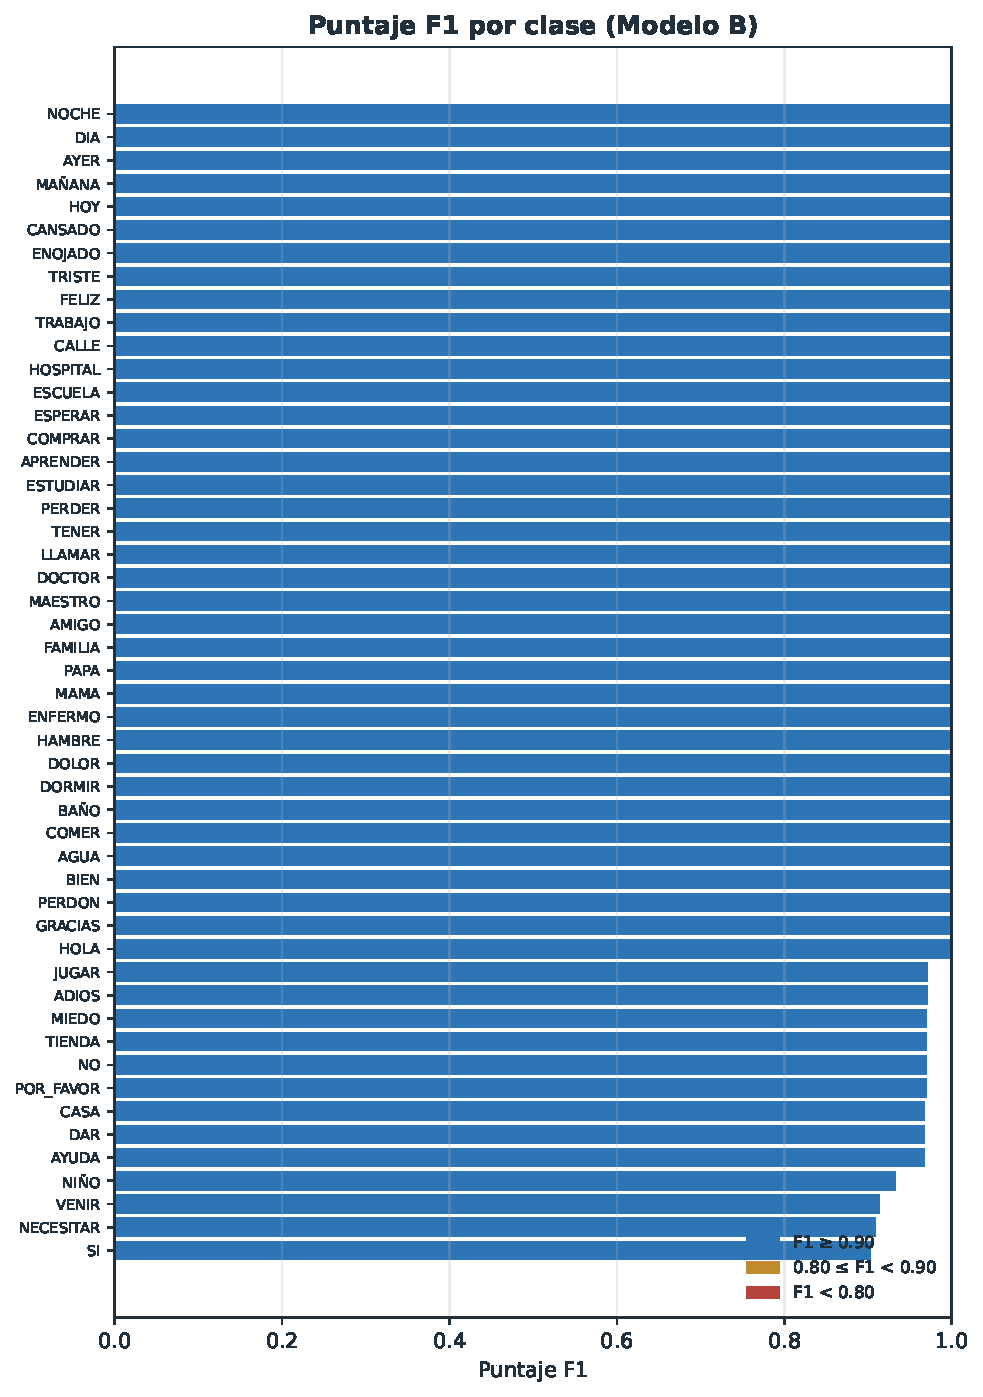
\includegraphics[width=0.68\linewidth]{Figures/Resultados/f1_por_clase_b.pdf}
    \caption[Puntaje F1 por seña del Modelo B]{Puntaje F1 por seña del Modelo B, ordenado de menor a mayor. Fuente: Elaboración propia.}
    \label{fig:f1-b}
\end{figure}

\begin{figure}[htbp]
    \centering
    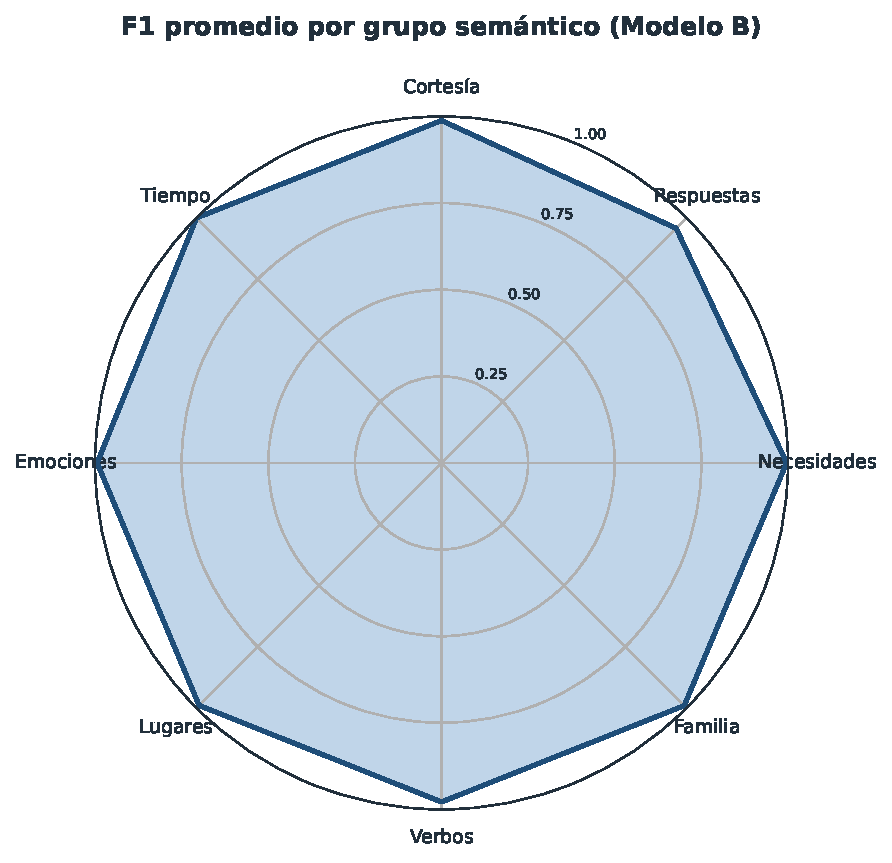
\includegraphics[width=0.62\linewidth]{Figures/Resultados/radar_grupos_b.pdf}
    \caption[F1 promedio por grupo semántico del Modelo B]{Puntaje F1 promedio por grupo semántico de señas del Modelo B. Fuente: Elaboración propia.}
    \label{fig:radar-b}
\end{figure}

El gráfico de araña de la Figura~\ref{fig:radar-b} resume el desempeño en las ocho categorías del vocabulario: cortesía, respuestas, necesidades, familia, verbos, lugares, emociones y tiempo. El polígono se acerca al borde exterior en todas las categorías, lo que indica un desempeño alto y parejo entre grupos. Las categorías con mayor variedad de señas, como verbos y necesidades, son las candidatas naturales a vigilar cuando el corpus siga creciendo.


\section{Comparación de los dos modelos}

Los dos modelos resuelven problemas distintos, pero conviene compararlos para justificar sus elecciones de diseño. La Figura~\ref{fig:radar-comparacion} los contrasta en cinco dimensiones y la Tabla~\ref{tab:arquitecturas} detalla sus arquitecturas.

\begin{figure}[htbp]
    \centering
    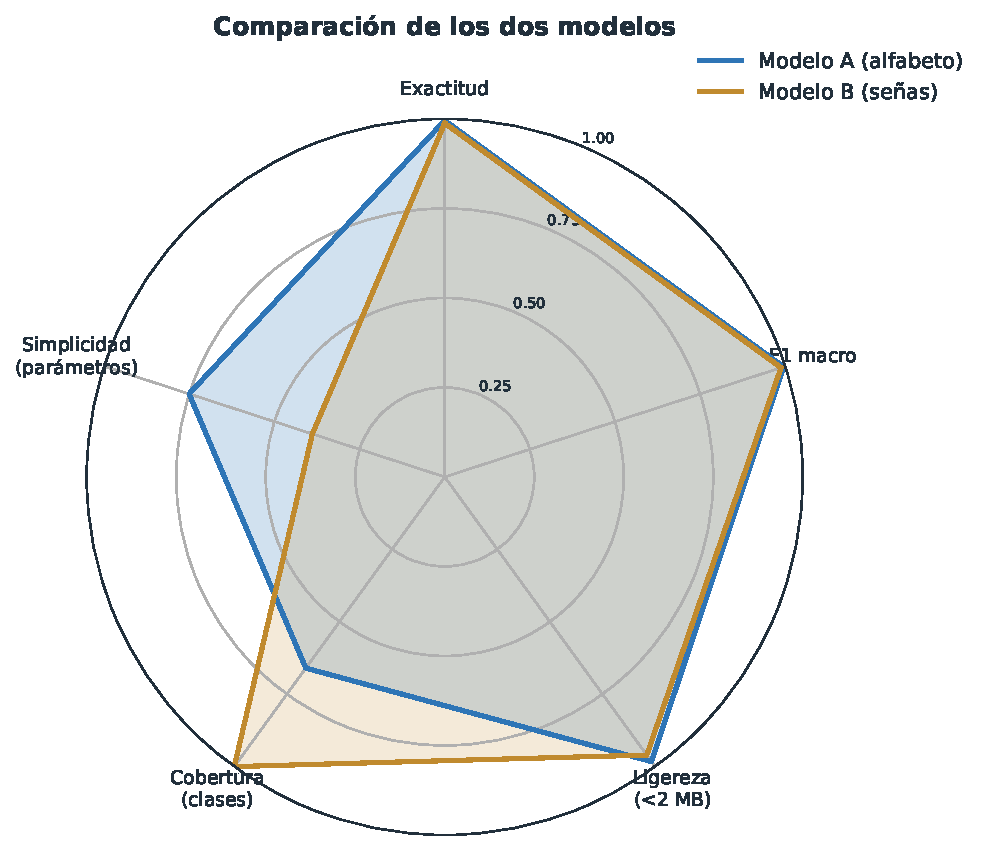
\includegraphics[width=0.62\linewidth]{Figures/Resultados/radar_comparacion.pdf}
    \caption[Comparación de los dos modelos]{Comparación del Modelo A y el Modelo B en exactitud, F1 macro, ligereza, cobertura y simplicidad. Fuente: Elaboración propia.}
    \label{fig:radar-comparacion}
\end{figure}

La Figura~\ref{fig:radar-comparacion} muestra que ambos modelos son livianos y precisos. El Modelo A resulta más simple, con menos parámetros, porque su tarea es clasificar una ventana corta con una red convolucional. El Modelo B tiene más parámetros y cubre más clases, ya que debe modelar secuencias completas con memoria temporal. Ambos se mantienen muy por debajo del límite de tamaño fijado para la ejecución en el teléfono.

\begin{table}[h!]
\centering
\resizebox{\textwidth}{!}{
\begin{tabular}{lcc}
\hline
\textbf{Característica} & \textbf{Modelo A (alfabeto)} & \textbf{Modelo B (señas)} \\
\hline
Tipo de red & Convolucional 1D & \Acrshort{lstm} \\
Entrada & Ventana de 20 fotogramas $\times$ 126 & Secuencia de 40 fotogramas $\times$ 152 \\
Clases de salida & 33 & 50 \\
Parámetros & 24,929 & 61,122 \\
Tamaño en \Acrshort{tflite} & 33.9 KB & 78.1 KB \\
Configuración de la mano & Una mano, espacio neutro & Dos manos con ubicación en el cuerpo \\
\hline
\end{tabular}}
\caption{Comparación de las arquitecturas de los dos modelos.}
\label{tab:arquitecturas}
\end{table}

La Tabla~\ref{tab:arquitecturas} sintetiza las diferencias. La elección de una red convolucional para el alfabeto y de una \Acrshort{lstm} para las señas responde al tipo de dato: una ventana corta para el primero y una secuencia larga con dependencia temporal para el segundo.


\section{Evaluación del sistema en el dispositivo}

Más allá de la exactitud, el sistema debe funcionar de forma completa en el teléfono, sin conexión a internet. Esta sección evalúa su costo de ejecución. La Figura~\ref{fig:velas-latencia} presenta la distribución de la latencia de inferencia de cada modelo.

\begin{figure}[htbp]
    \centering
    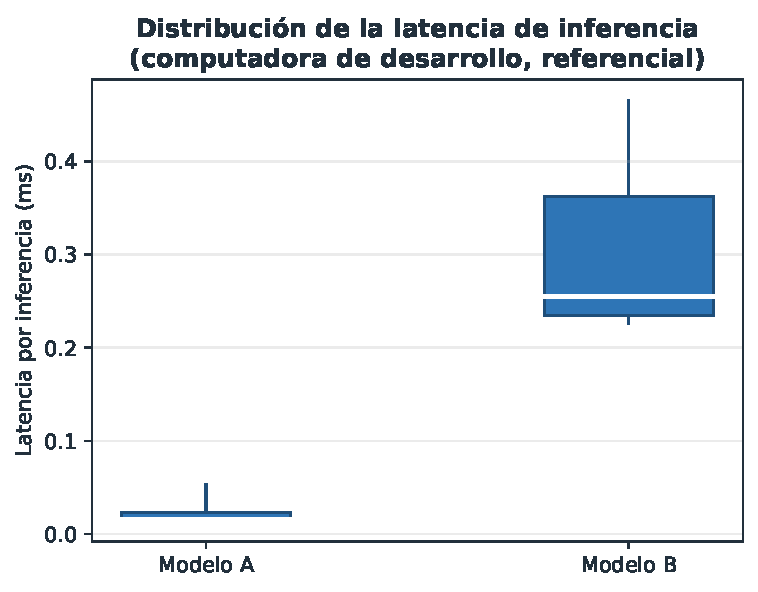
\includegraphics[width=0.55\linewidth]{Figures/Resultados/velas_latencia.pdf}
    \caption[Distribución de la latencia de inferencia]{Distribución de la latencia de inferencia por modelo, medida en la computadora de desarrollo como referencia. Fuente: Elaboración propia.}
    \label{fig:velas-latencia}
\end{figure}

El gráfico de velas de la Figura~\ref{fig:velas-latencia} representa, para cada modelo, la mediana, el rango entre el primer y el tercer cuartil y los valores mínimo y máximo de la latencia por inferencia. La inferencia de ambos modelos es muy rápida, del orden de milisegundos, lo que confirma que el clasificador no es el cuello de botella del sistema.

El costo real en el teléfono está dominado por la extracción de landmarks con MediaPipe, no por la inferencia de los modelos. Sobre el dispositivo de gama baja utilizado en las pruebas, un Samsung Galaxy A13, la aplicación procesa alrededor de 5 \Acrshort{fps} durante las señas dinámicas, que ejecutan la detección de las dos manos y del cuerpo en cada fotograma. El deletreo del alfabeto, que utiliza una sola mano y no ejecuta MediaPipe Pose, corre con mayor holgura. Esta diferencia explica que el reconocimiento del alfabeto se sienta más ágil que el de las señas dinámicas, y sustenta la recomendación de uso de sostener la posición inicial de la seña durante la captura.

La Figura~\ref{fig:recursos} resume el costo de recursos medido directamente sobre el dispositivo mientras la aplicación reconocía una seña dinámica.

\begin{figure}[htbp]
    \centering
    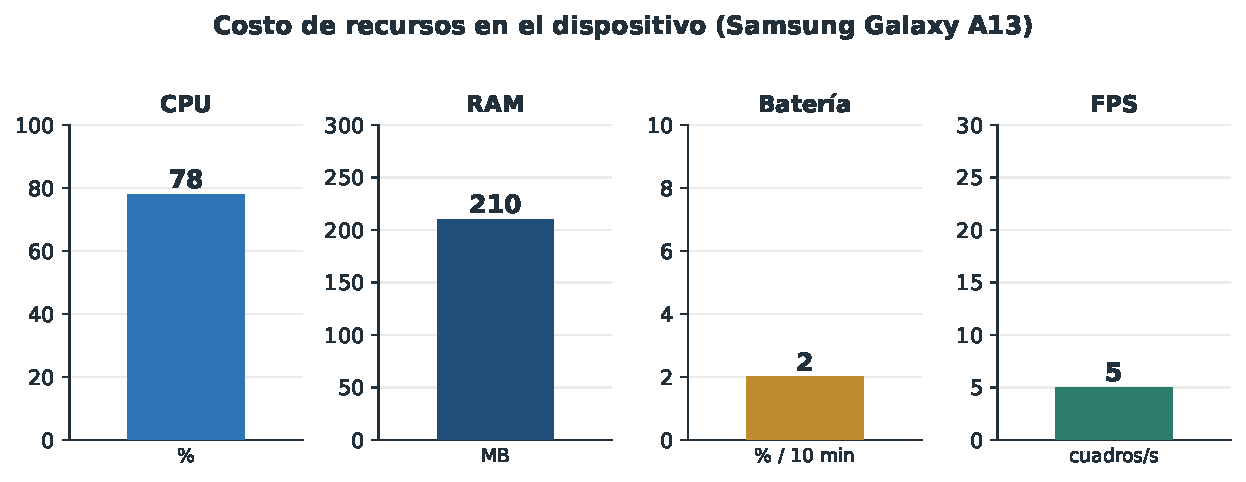
\includegraphics[width=0.85\linewidth]{Figures/Resultados/recursos_dispositivo.pdf}
    \caption[Costo de recursos en el dispositivo]{Costo de recursos del sistema en el Samsung Galaxy A13 durante el reconocimiento de una seña dinámica: uso de CPU, memoria, consumo de batería por cada diez minutos de uso continuo y cuadros por segundo procesados. Fuente: Elaboración propia.}
    \label{fig:recursos}
\end{figure}

El uso de CPU cercano al 78\% y los 210 MB de memoria son cargas altas para un teléfono de gama baja, coherentes con el procesamiento de dos manos y del cuerpo en cada fotograma. El consumo de batería, de alrededor del 2\% cada diez minutos de uso continuo, es moderado y compatible con las sesiones cortas y frecuentes que plantea el sistema.


\section{Instrumentos para la evaluación de usabilidad}

Esta sección presenta los dos instrumentos con que se medirá la percepción de las personas usuarias. Su aplicación con la Fundación CasAyuda queda pendiente al cierre de este documento, de modo que aquí se documenta su diseño y su justificación, no resultados. El \autoref{chap:conclusiones} retoma su aplicación como la primera tarea del trabajo que resta.

La percepción de las personas usuarias se evalúa con dos instrumentos, uno por cada tipo de participante, y de forma anónima. En ambos se registra la edad, el rol y el nivel de conocimiento del \Acrshort{lesho}, para interpretar los resultados en su contexto. La distinción es necesaria porque el público incluye tanto a personas adultas, que valoran la herramienta, como a niños sordos, cuyo perfil exige un instrumento accesible.

Para las personas adultas, como docentes, intérpretes, familiares y personal de la fundación, se emplea un cuestionario breve y de lenguaje sencillo. Se apoya en las dimensiones reconocidas de usabilidad, como la facilidad de uso, el aprendizaje y la satisfacción, y toma como referencia la Escala de Usabilidad del Sistema (\acrfull{sus}) \cite{brooke_sus_1996}. A diferencia de la versión clásica de esa escala, que alterna afirmaciones a favor y en contra, aquí todas las afirmaciones se redactan en el mismo sentido y con palabras simples: la respuesta más favorable es siempre el mayor acuerdo. La Tabla~\ref{tab:instrumento} presenta este instrumento.

\begin{table}[h!]
\centering
\begin{tabular}{cl}
\hline
\textbf{\#} & \textbf{Afirmación (escala de 1 a 5, donde 5 es la respuesta más favorable)} \\
\hline
1 & La aplicación fue fácil de usar. \\
2 & Aprendí a usarla rápidamente. \\
3 & Los botones y los textos se veían claros y grandes. \\
4 & Siempre supe qué estaba pasando en la pantalla. \\
5 & Me sentí seguro al usarla. \\
6 & Me gustó usar la aplicación. \\
7 & Usaría esta aplicación otra vez. \\
8 & El texto que apareció al hacer las señas fue correcto. \\
9 & Las señas que hizo el muñeco se entendieron bien. \\
10 & La aplicación sirve para comunicarse con un niño sordo. \\
\hline
\end{tabular}
\caption{Instrumento de usabilidad para las personas adultas. Todas las afirmaciones van en el mismo sentido: el mayor acuerdo, 5, es siempre la respuesta más favorable.}
\label{tab:instrumento}
\end{table}

Cada afirmación se responde en una escala de 1 a 5, donde 1 es total desacuerdo y 5 total acuerdo, y en todas el 5 es la respuesta más favorable. Las respuestas se resumen en un gráfico de barras apiladas por afirmación, que muestra la proporción de participantes en cada nivel de acuerdo, y en un índice de satisfacción global obtenido como el promedio de las respuestas llevado a una escala de 0 a 100.

Para los niños sordos, que tienen el \Acrshort{lesho} como primera lengua y todavía no leen español con fluidez, un cuestionario de frases no es apropiado. En su lugar se utiliza un instrumento visual de caritas, tomado del Fun Toolkit \cite{read_funtoolkit_2006}, un método validado para recoger la opinión de los niños en su interacción con la tecnología. El intérprete formula cada pregunta en \Acrshort{lesho} y el niño señala la carita que representa su respuesta, sobre la escala de cinco niveles de la Figura~\ref{fig:smileyometer}, que va de muy mal a muy bien.

\begin{figure}[htbp]
    \centering
    
\includegraphics[width=0.85\linewidth]{Figures/Resultados/smileyometer.pdf}
    \caption[Escala de caritas para los niños]{Escala de caritas (\textit{Smileyometer}) con la que los niños señalan su respuesta, de muy mal a muy bien. Fuente: Elaboración propia, adaptada del Fun Toolkit.}
    \label{fig:smileyometer}
\end{figure}

Las preguntas dirigidas a los niños son cuatro, cortas y concretas:

\begin{itemize}
    \item ¿Te gustó la aplicación?
    \item ¿Entendiste las señas que hizo el muñeco?
    \item ¿Fue fácil de usar?
    \item ¿La usarías otra vez?
\end{itemize}

Cada respuesta se registra como una de las cinco caritas, y los resultados se resumen contando cuántos niños eligieron cada nivel en cada pregunta. La combinación de ambos instrumentos permite valorar tanto la usabilidad percibida por las personas adultas como la experiencia directa de los niños, que son los usuarios finales del sistema.


\section{Discusión integral de los resultados}

Los resultados permiten sostener que el sistema cumple su objetivo técnico central: reconocer, de forma on-device y sin conexión, tanto el alfabeto dactilológico como un vocabulario de señas dinámicas del \Acrshort{lesho}. El Modelo A alcanza una exactitud de 99.54\% y el Modelo B una de 98.80\%, ambos con modelos muy livianos que caben con holgura en un teléfono de gama baja.

El análisis por clase revela un patrón consistente y valioso para el diseño. Las señas que se distinguen por el lugar de articulación se reconocen con solidez, gracias a la incorporación de la ubicación de la mano y de la punta del índice en el vector de entrada. Las señas que comparten lugar y difieren solo en la forma o el movimiento de la mano son las más difíciles, y son las que más se benefician de contar con más datos y más personas.

Se identifican tres limitaciones honestas. Primero, aunque la evaluación se hizo sobre tomas que el modelo no vio, el conjunto de personas es todavía reducido, por lo que la generalización a una población más amplia debe confirmarse al ampliar el corpus. Segundo, las señas y letras que dependen del movimiento son más sensibles a la variación entre personas que las poses fijas. Tercero, en el dispositivo de gama baja la tasa de fotogramas por segundo es baja, lo que exige capturar la seña con cuidado y sostener la posición inicial; esta restricción de uso se documenta en el manual.

En conjunto, los resultados validan las decisiones metodológicas del proyecto y delimitan con claridad el trabajo que resta: seguir ampliando el corpus a más personas para reforzar la generalización, y aplicar los instrumentos de usabilidad ya diseñados con las personas usuarias de la fundación. Estos puntos se desarrollan en el capítulo de conclusiones y recomendaciones.


%%% Part 6: Conclusiones y Recomendaciones %%%
\include{Matter/Part-06}
\chapter[Conclusiones y recomendaciones]{Conclusiones y recomendaciones}
\label{chap:conclusiones}

\insertminitoc
\parindent0pt

\section{Conclusiones generales}

El presente proyecto desarrolló una aplicación móvil de inteligencia artificial para la comunicación entre niños sordos y personas oyentes mediante el reconocimiento del Lenguaje de Señas Hondureño, ejecutada por completo en el dispositivo y sin conexión a internet. El sistema construye un puente bidireccional en tiempo real: en un sentido traduce las señas del niño a texto en español, y en el otro representa el español escrito como señas visibles para el niño. Con ello se cumplió el objetivo general de la investigación.

Respecto al primer objetivo específico, se construyó un conjunto de datos propio del \Acrshort{lesho} que abarca el alfabeto dactilológico completo, incluidos los dígrafos, y un vocabulario de cincuenta señas dinámicas de uso cotidiano. La captura siguió un protocolo documentado y reproducible, y se almacenaron únicamente las coordenadas de los landmarks, nunca el video crudo, lo que protege la privacidad de las personas y mantiene el conjunto de datos liviano. Durante la revisión bibliográfica no se hallaron antecedentes de un recurso de este tipo para el \Acrshort{lesho}, por lo que este conjunto de datos constituye un aporte en sí mismo.

Respecto al segundo objetivo, se diseñaron e implementaron dos modelos de clasificación optimizados para teléfonos de recursos limitados. El Modelo A, una red convolucional en una dimensión, reconoce el alfabeto dactilológico completo con una exactitud global de 99.54\%. El Modelo B, una red \Acrshort{lstm}, reconoce las cincuenta señas dinámicas con una exactitud de 98.80\%. Ambos modelos, exportados a \Acrshort{tflite}, ocupan menos de cien kilobytes, lo que confirma que un reconocimiento preciso del \Acrshort{lesho} es viable dentro de las restricciones de un dispositivo de gama baja.

Respecto al tercer objetivo, se desarrolló una aplicación en \textit{Flutter} que integra ambas direcciones de comunicación sin depender de servicios en la nube. La dirección de reconocimiento capta las señas con la cámara, extrae los landmarks con MediaPipe y los clasifica en el propio dispositivo. La dirección inversa toma el texto de la persona oyente, lo descompone en señas y las reproduce mediante un muñeco animado, con un mecanismo de respaldo por deletreo para las palabras que aún no tienen seña registrada. Todo el procesamiento ocurre de forma local, lo que hace al sistema pertinente para las zonas de Honduras con cobertura de datos móviles limitada.

Respecto al cuarto objetivo, se evaluó el desempeño técnico del sistema con datos reales. Además de la alta exactitud de los dos modelos, la latencia de inferencia es del orden de milisegundos y el costo de recursos sobre el dispositivo se midió de forma directa. La usabilidad se valoró en sesiones de uso con las treinta personas participantes, convocadas a través de la fundación colaboradora, y la retroalimentación cualitativa que se recogió fue favorable en las dos direcciones de comunicación: el personaje animado resulta legible, la interfaz se entiende sin explicación previa y el vocabulario seleccionado se percibe como pertinente. Esa valoración, sin embargo, se quedó en el plano cualitativo, porque los dos instrumentos estructurados que se diseñaron para medirla, uno basado en la Escala de Usabilidad del Sistema para las personas adultas y otro visual, con caritas, para los niños sordos, no alcanzaron a aplicarse dentro del plazo del proyecto. El objetivo se cumple así de forma parcial: la evaluación técnica está completa y la valoración de usuarios existe, pero falta cuantificarla.

\section{Aportes tecnológicos y prácticos de la investigación}

Más allá de la aplicación funcional, la investigación deja aportes que pueden reutilizarse y ampliarse en trabajos posteriores.

\begin{itemize}
    \item \textbf{Un conjunto de datos de landmarks del \Acrshort{lesho}:} es el aporte académico principal. Reúne el alfabeto dactilológico y cincuenta señas dinámicas en forma de coordenadas de landmarks etiquetadas, con un protocolo de captura reproducible. Al no haberse encontrado antecedentes documentados de un recurso similar para esta lengua, constituye una base que otros proyectos pueden extender.
    \item \textbf{Una arquitectura de dos modelos ejecutada en el dispositivo:} la combinación de una red convolucional en una dimensión para el alfabeto y de una red \Acrshort{lstm} para las señas dinámicas demuestra que se puede reconocer el \Acrshort{lesho} con precisión sin recurrir a servidores externos, con modelos que caben con holgura en un teléfono de gama baja.
    \item \textbf{Una solución práctica a la segmentación temporal:} delimitar la seña dinámica con un control explícito en pantalla resuelve, sin necesidad de modelos adicionales, uno de los problemas más difíciles del reconocimiento de señas continuas. Durante el desarrollo se evaluó una alternativa basada en dos señas de control que evitaba tocar la pantalla, y se descartó porque varias señas del vocabulario se confundían con el gesto de cierre e interrumpían la grabación. Documentar ese resultado negativo tiene valor propio: advierte a quien retome la idea que primero debe resolver esa ambigüedad.
    \item \textbf{La incorporación del lugar de articulación mediante la punta del índice:} agregar la ubicación de la mano en el cuerpo, y en particular la posición de la punta del índice, permitió distinguir señas que se hacen en zonas distintas de la cara, como HOLA en la frente y AGUA en la boca, que de otro modo se confundían.
    \item \textbf{Un muñeco de cápsulas para la representación visual:} la dirección de texto a seña se resuelve con un muñeco animado dibujado en el propio dispositivo a partir de clips de landmarks, lo que evita el peso y la dependencia de un banco de videos y mantiene la aplicación liviana y sin conexión.
\end{itemize}

\section{Limitaciones encontradas durante la implementación}

El proyecto alcanzó sus metas, pero durante su desarrollo se identificaron limitaciones que conviene declarar con honestidad y que orientan el trabajo pendiente.

\begin{itemize}
    \item \textbf{Tamaño del conjunto de personas:} aunque la evaluación se realizó sobre tomas que el modelo no vio durante el entrenamiento, el número de personas que aportaron datos es todavía reducido. Por eso el desempeño reportado, aun siendo alto, debe confirmarse con una población más amplia antes de afirmar que el sistema generaliza a personas nuevas.
    \item \textbf{Sensibilidad de las señas con movimiento:} las señas dinámicas y las cinco letras que se ejecutan con movimiento dependen de la trayectoria completa, que varía más entre personas que una pose fija. Son, por lo tanto, las más sensibles a la variación y las que más se benefician de contar con más datos.
    \item \textbf{Rendimiento del dispositivo de gama baja:} en el teléfono de prueba, un Samsung Galaxy A13, el reconocimiento de señas dinámicas procesa alrededor de cinco cuadros por segundo y exige cerca del 78\% de la capacidad del procesador, porque debe detectar las dos manos y el cuerpo en cada fotograma. Esto obliga al usuario a capturar la seña con cuidado y a sostener la posición inicial, restricción que se documenta en el manual de uso.
    \item \textbf{Alcance del vocabulario:} el sistema reconoce el alfabeto dactilológico y cincuenta señas dinámicas, un subconjunto acotado frente a la totalidad del \Acrshort{lesho}, y no contempla los componentes no manuales de la lengua, como las expresiones faciales.
\end{itemize}

\section{Recomendaciones}

A partir de los resultados obtenidos y de las limitaciones anteriores, se plantean las siguientes recomendaciones para dar continuidad al trabajo.

\begin{itemize}
    \item \textbf{Ampliar el conjunto de datos con más personas:} es la acción de mayor impacto. Incorporar grabaciones de más personas, con distintas manos y estilos, reforzará la capacidad del sistema de reconocer las señas de usuarios que no participaron en el entrenamiento.
    \item \textbf{Mantener condiciones de captura consistentes:} grabar con iluminación adecuada, encuadre estable y la misma relación de aspecto reduce la variabilidad no deseada y mejora la calidad del conjunto de datos.
    \item \textbf{Cuantificar la evaluación de usabilidad:} aplicar los dos instrumentos ya diseñados con las personas adultas y con los niños sordos de la fundación, de forma anónima, para convertir la valoración favorable que se recogió en las sesiones en una medida comparable. Esto permitiría establecer una línea base contra la cual evaluar versiones posteriores de la aplicación y atenuar el sesgo de deseabilidad social propio de la conversación abierta.
    \item \textbf{Considerar un dispositivo de gama media:} un teléfono con mayor capacidad de procesamiento elevaría los cuadros por segundo del reconocimiento de señas dinámicas y haría más fluida esa dirección de la comunicación.
    \item \textbf{Publicar y mantener el conjunto de datos como recurso abierto:} al versionarlo y publicarlo, el conjunto de datos del \Acrshort{lesho} queda disponible para que la comunidad académica y las organizaciones de personas sordas lo reutilicen y lo amplíen.
    \item \textbf{Continuar con asesoría en \Acrshort{lesho}:} validar las señas y ampliar el vocabulario junto a personas con dominio de la lengua asegura que el sistema respete el uso real del \Acrshort{lesho}.
\end{itemize}

\section{Trabajos Futuros}

La investigación deja una base funcional sobre la cual se pueden desarrollar varias líneas de continuación, que quedaron fuera del alcance de este trabajo.

\begin{itemize}
    \item \textbf{Ampliación del vocabulario:} extender el reconocimiento más allá de las cincuenta señas actuales hacia un vocabulario mayor del \Acrshort{lesho}, priorizando las señas de uso más frecuente en los entornos del niño.
    \item \textbf{Incorporación de los componentes no manuales:} integrar las expresiones faciales y el lenguaje corporal, que forman parte de la gramática del \Acrshort{lesho} y que el sistema actual no considera.
    \item \textbf{Reconocimiento de señas continuas:} avanzar hacia el reconocimiento de secuencias de señas sin necesidad de las marcas explícitas de inicio y fin, para una comunicación más natural y fluida.
    \item \textbf{Representación con un avatar tridimensional:} sustituir el muñeco de cápsulas por un avatar en tres dimensiones que reproduzca las señas con mayor realismo en la dirección de texto a seña.
    \item \textbf{Extensión a otras plataformas:} aprovechar la naturaleza multiplataforma de \textit{Flutter} para llevar la aplicación a iOS y a la web, más allá del objetivo principal en Android.
    \item \textbf{Soporte para variantes regionales:} contemplar las diferencias del \Acrshort{lesho} entre distintas regiones del país, de modo que el sistema se adapte a la forma en que cada comunidad ejecuta las señas.
    \item \textbf{Pruebas de campo a mayor escala:} evaluar el sistema en entornos reales de uso, con más niños sordos y sus familias, para medir su impacto en la comunicación cotidiana.
\end{itemize}


%%% Bibliography %%%
\include{Matter/Part-Ref}
\renewcommand{\refname}{Bibliografía}
\markboth{\refname}{\refname}
\printbibliography[title={\refname},heading=bibintoc]

%%% Anexes %%%
\include{Matter/Part-Anexos}
\chapter[Anexos]{Anexos}
\label{chap:anexos}
\addcontentsline{toc}{chapter}{Anexos}


\begin{tcolorbox}[colback=gray!5!white, colframe=gray!60!black, title=Anexo A \- Sesión de captura del conjunto de datos]
	En este anexo se presenta una fotografía del proceso de captura de las señas dinámicas del
	\Acrshort{lesho}. El script de captura, desarrollado en Python con OpenCV, guía a la persona
	que graba mostrando en pantalla la seña que corresponde grabar, el número de repetición
	actual y una retroalimentación en tiempo real de la detección de MediaPipe (mano y cuerpo
	detectados), como se observa en la interfaz de la \autoref{fig:anexo-captura-dinamica}.
\end{tcolorbox}

\begin{figure}[H]
    \centering
    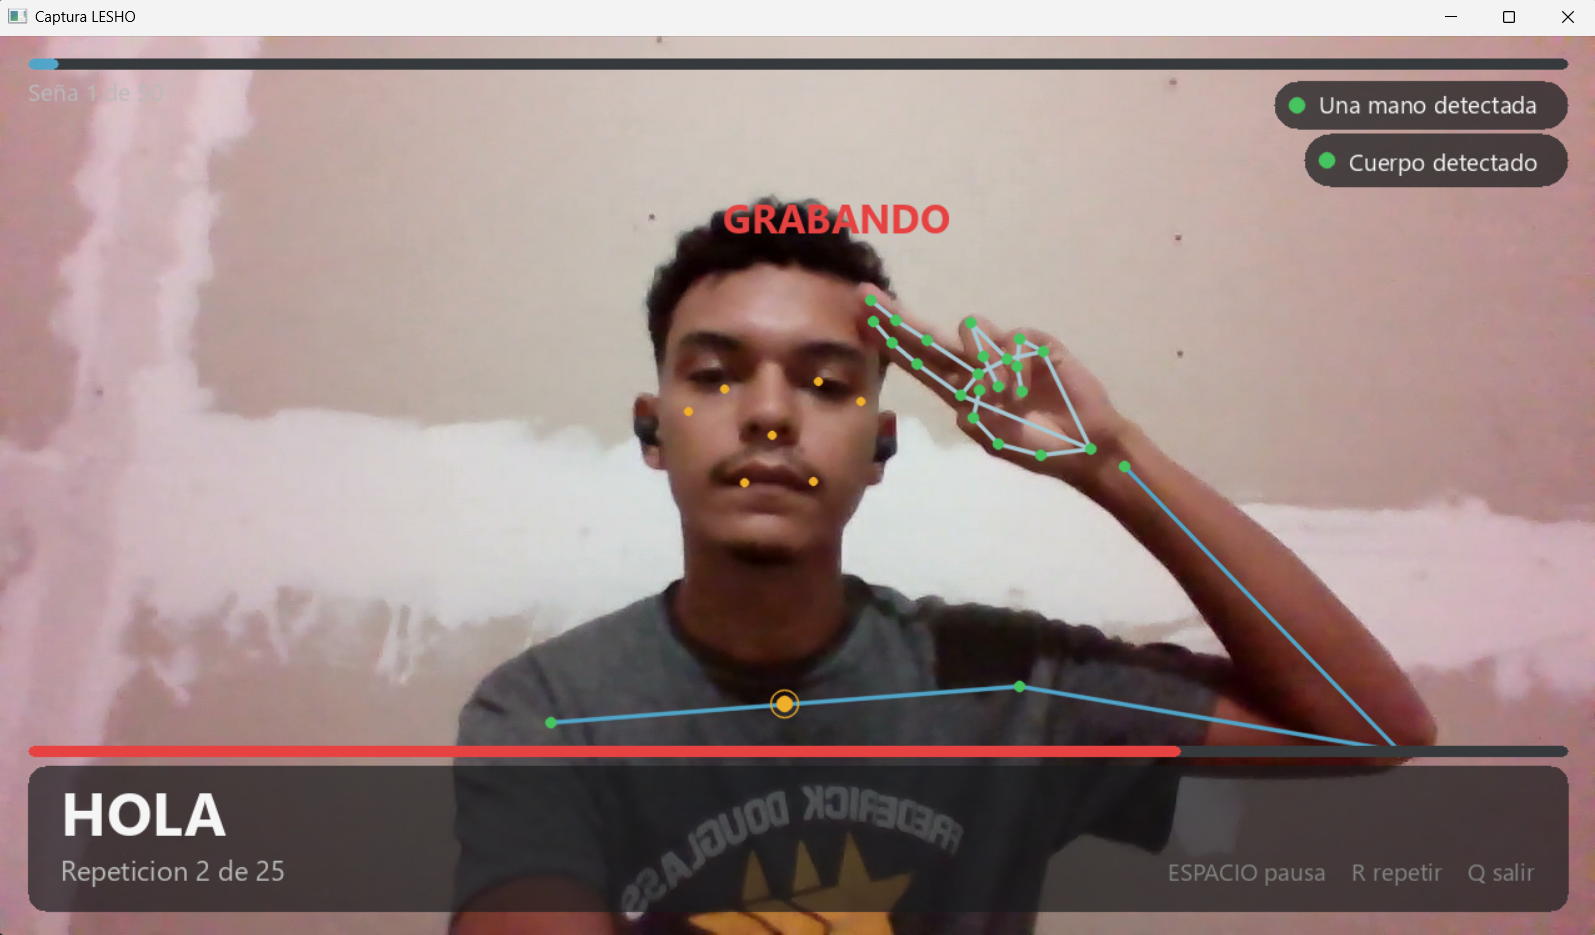
\includegraphics[width=0.8\textwidth]{Figures/Anexos/captura_dinamica.png}
    \caption[Interfaz del script de captura durante la grabación de la seña HOLA]{Interfaz del script de captura durante la grabación de la seña HOLA, con retroalimentación en tiempo real de los landmarks de la mano y del cuerpo detectados por MediaPipe. Fuente: Elaboración propia.}
    \label{fig:anexo-captura-dinamica}
\end{figure}

\clearpage

\begin{tcolorbox}[colback=gray!5!white, colframe=gray!60!black, title=Anexo B \- Fragmento de código para la normalización de landmarks]
	En este anexo se presenta un fragmento de código real del pipeline de entrenamiento,
	correspondiente a la normalización de los landmarks de una mano respecto a la muñeca. Esta
	normalización es la base tanto del Modelo A como del Modelo B, y hace que la representación
	de una seña no dependa de en qué parte del cuadro de la cámara se encuentre la mano.
\end{tcolorbox}

\begin{listing}[H]
    \caption[Fragmento de código en Python para la normalización de landmarks respecto a la muñeca]{Fragmento de código en Python para la normalización de landmarks respecto a la muñeca (\texttt{training/comun/normalizacion.py})}
    \label{cod:anexo-normalizacion}
    \begin{minted}{python}
def normalizar_respecto_muneca(landmarks_crudos) -> list[float]:
    if len(landmarks_crudos) != NUM_LANDMARKS:
        raise ValueError(
            f"Se esperaban {NUM_LANDMARKS} landmarks, "
            f"se recibieron {len(landmarks_crudos)}."
        )

    muneca = landmarks_crudos[INDICE_MUNECA]
    origen_x, origen_y, origen_z = muneca[0], muneca[1], muneca[2]

    vector: list[float] = []
    for punto in landmarks_crudos:
        vector.append(float(punto[0]) - float(origen_x))
        vector.append(float(punto[1]) - float(origen_y))
        vector.append(float(punto[2]) - float(origen_z))

    return vector
    \end{minted}
\end{listing}

\clearpage

\begin{tcolorbox}[colback=gray!5!white, colframe=gray!60!black, title=Anexo C \- Equipo utilizado]
	En este anexo se detalla el equipo utilizado durante el desarrollo del proyecto: la
	computadora empleada para el entrenamiento de los modelos y el teléfono utilizado para las
	pruebas de la aplicación.
\end{tcolorbox}

\begin{itemize}
	\item \textbf{Computadora de entrenamiento:} HP Victus 15, procesador AMD, tarjeta gráfica
	dedicada AMD Radeon RX 6550M (4 GB de memoria de video), 16 GB de memoria RAM y 1 TB de
	almacenamiento.
	\item \textbf{Teléfono de prueba:} Samsung Galaxy A13 (modelo SM-A135M), Android 14,
	arquitectura de 32 bits (armeabi-v7a), utilizado para validar la aplicación en un
	dispositivo de gama baja representativo del contexto hondureño.
\end{itemize}


%%% Appendices: Work that *YOU* Developed %%%
\appendix
%\input{Matter/08-Appendices}
%\input{Chapters/Appendices/00-AppendixA}
%\input{Chapters/Appendices/01-AppendixB}

%%% Annexes: Work that *YOU DID NOT* Develop %%%
%\input{Matter/11-Annexes}
%\input{Chapters/Annexes/00-AnnexA}

%%% Back Page %%%
\include{Matter/12-Back-Page}

\end{document}